%%%%%%%%%%%%%%%%%%%%%%%%%%%%%%%%%%%%%%%%%%%%%%%%%%%%%%%%%%%%%%%%%%%%%%
% Lớp 11 | Quan hệ vuông góc trong không gian | Góc giữa đường thẳng và mặt phẳng. Góc nhị diện
% Dạng 1H8?6-2: Góc nhị diện, góc phẳng nhị diện
% Số câu: 117  (sinh tự động bởi tach_cau.py; từ nay thầy sửa trực tiếp file này)
%%%%%%%%%%%%%%%%%%%%%%%%%%%%%%%%%%%%%%%%%%%%%%%%%%%%%%%%%%%%%%%%%%%%%%

%%%%%%%%%%%%%%%% TRẮC NGHIỆM 4 PHƯƠNG ÁN %%%%%%%%%%%%%%%%

% nguồn: Ok_Toan11_TracNghiem_Lan2
\begin{ex}%[1H8N6-2]%[ma:2b87734d]
	Cho hình lăng trụ đứng $ABC.A'B'C'$ có đáy $ABC$ là tam giác vuông tại $A$. Góc phẳng nhị diện $\left[B,  AA', C\right]$ có số đo bằng
	\choice 
		{$30^{\circ}$} 
		{$45^{\circ}$} 
		{$60^{\circ}$} 
		 {\True $90^{\circ}$}
	 \loigiai{
		\begin{center}
			\begin{tikzpicture}[scale=1,line cap=round,line join=round,font=\footnotesize,declare function={a=3.5; b=1.5; h=3.5; goc=-120;}]
					 \path
						 (0:0) coordinate (A)
						 (0:a) coordinate (C)
						(goc:b)  coordinate (B)
						(0,h) coordinate (A') 
						($(B)+(0,h)$) coordinate (B') 
						($(C)+(0,h)$) coordinate (C'); 
					 \draw[dashed]
						(A)--(C) 
						 (A')--(A)--(B);
					 \draw
						(A')--(B')--(C')--(C)--(B)--(B') 
						 (A')--(C')
						 (B)--(B')
					\foreach \x/\y/\z in {B'/A'/C',B/A/C}{ 
						pic[draw,angle radius = 6pt]{right angle  = \x--\y--\z}
						 };
					\foreach \x/\g  in {A/180,B/180,C/0,A'/-180,B'/180,C'/0}
					\fill (\x) circle (1pt) 
						 +(\g:3mm) node {$\x$};
				\end{tikzpicture}
		\end{center}
		Ta có $BA\perp AA'$ và $CA\perp  AA'$ suy ra $\widehat{BAC}$ là góc phẳng nhị diện $\left[B, AA', C\right]$ và bằng $90^{\circ}$.
	} 
\end{ex}

% nguồn: Ok_Toan11_TracNghiem_Lan2
\begin{ex}%[1H8N6-2]%[ma:f5d32bb9]
	Cho hình chóp $S.ABCD$  có đáy $ABCD$ là hình chữ nhật tâm $O$, $SA\perp \left(ABCD\right)$. Gọi $H$ là hình chiếu của $S$ lên $BD$. Góc phẳng nhị diện $\left[S, BD, A\right]$ là
	\choice 
		 {$\widehat{SOA}$}
		 {$\widehat{SBA}$}
		 {\True $\widehat{SHA}$}
		 {$\widehat{SDA}$}
	 \loigiai{
		\begin{center}
			\begin{tikzpicture}[line cap=round,line join=round,font=\footnotesize,declare function={a=4; b=2; h=3.5; goc=-135;}]
					 \path
						(0:0) coordinate  (A)
						(0:a) coordinate (B) 
						(goc:b) coordinate  (D)
						 ($(B)+(D)-(A)$) coordinate (C)
						($(A)!0.5!(C)$) coordinate (O) 
						(0,h) coordinate (S) 
						 ($(D)!0.4!(B)$) coordinate (H);
					\draw[dashed] 
						(A)--(B) 
						 (A)--(D)--(B)
						(C)--(A)--(S)--(H)--(A); 
					 \draw
						(D)--(C)--(B) 
						 (S)--(B)
						 (S)--(C)
						(S)--(D) 
					\foreach  \x/\y/\z in {S/A/B,S/A/D,A/H/D}{
						pic[draw,angle radius = 6pt]{right  angle = \x--\y--\z}
						}; 
					\foreach  \x/\g in {A/135,B/0,C/-45,D/-135,S/90,O/-90,H/-90}
					\fill (\x) circle  (1pt)
						 +(\g:3.5mm) node {$\x$};
				\end{tikzpicture}
		\end{center}
		Ta có $SH\perp BD$ và $AH\perp BD$ suy ra $\widehat{SHA}$ là góc phẳng nhị diện $\left[S,  BD, A\right]$.
	} 
\end{ex}

% nguồn: Ok_Toan11_TracNghiem_Lan2
\begin{ex}%[1H8N6-2]%[ma:32931767]
	 Cho hình chóp tứ giác đều $S.ABCD$. Phát biểu nào sau đây là đúng?
	\choice 
		{Số đo  của góc nhị diện $[S,AB,C]$ bằng $\widehat{SBC}$}
		{Số đo của góc  nhị diện $[D,SA,B]$ bằng $90^{^{\circ}}$}
		{\True Số đo của góc nhị diện $[S,AC,B]$  bằng $90^{^{\circ}}$}
		 {Số đo của góc nhị diện $[D,SA,B]$ bằng $\widehat{BSD}$}
	\loigiai{ 
		\begin{center}
			\begin{tikzpicture}[line cap=round,line join=round,font=\footnotesize,declare function={a=3.5; b=2; h=3.5; goc=-135;}]
					 \path
						(0:0) coordinate (A) 
						 (0:a) coordinate (B)
						(goc:b) coordinate  (D)
						($(B)+(D)-(A)$)  coordinate (C)
						($(A)!0.5!(C)$) coordinate  (O)++(0,h) coordinate (S);
					 \draw[dashed]
						 (A)--(B)
						(A)--(D)--(B) 
						 (C)--(A)--(S)--(O);
					\draw 
						(D)--(C)--(B) 
						 (S)--(B)
						 (S)--(C)
						 (S)--(D)
					\foreach \x/\y/\z in {S/O/B,S/O/A}{ 
						 pic[draw,angle radius = 6pt]{right angle = \x--\y--\z}
						}; 
					 \foreach \x/\g in {A/135,B/0,C/-45,D/-135,S/90,O/-90}
					 \fill (\x) circle (1pt)
						+(\g:3.5mm) node  {$\x$};
				\end{tikzpicture}
		\end{center}
		Gọi  $O=AC\cap BD$.\\
		Vì $S.ABCD$ là  hình chóp đều nên $SO\perp \left(ABCD\right) \Rightarrow SO\perp AC$, $SO\perp BD$, $AC\perp BD$.\\
		Do đó số đo của góc nhị  diện $[S,AC,B]=\widehat{SOB}=90^\circ$.
	} 
\end{ex}

% nguồn: Ok_Toan11_TracNghiem_Lan2
\begin{ex}%[1H8N6-2]%[ma:550074a1]
	Cho  hình chóp tứ giác đều $S.ABCD$. Phát biểu nào sau đây đúng?
	\choice 
		{Số  đo của góc nhị diện $\left[S,AB,C\right]$ bằng $\widehat{SBC}$}
		{Số đo của góc  nhị diện $\left[D,SA,B\right]$ bằng $90^{\circ}$}
		{\True Số đo của góc nhị diện $\left[S,AC,B\right]$ bằng $90^{\circ}$} 
		{Số đo của góc nhị diện $\left[D,SA,B\right]$ bằng  $\widehat{BSD}$}
	 \loigiai{
		\begin{center}
			\begin{tikzpicture}[line cap=round,line join=round,font=\footnotesize,declare function={a=3.5; b=2; h=3.5; goc=-135;}]
					\path 
						(0:0) coordinate  (A)
						(0:a)  coordinate (B)
						(goc:b) coordinate  (D)
						($(B)+(D)-(A)$)  coordinate (C)
						($(A)!0.5!(C)$) coordinate  (O)++(0,h) coordinate (S);
					 \draw[dashed]
						 (A)--(B)
						 (A)--(D)--(B)
						(C)--(A)--(S)--(O); 
					\draw 
						 (D)--(C)--(B)
						 (S)--(B)
						(S)--(C) 
						 (S)--(D)
					 \foreach \x/\y/\z in {S/O/B,S/O/A}{
						pic[draw,angle radius = 6pt]{right angle =  \x--\y--\z}
						}; 
					\foreach \x/\g in  {A/135,B/0,C/-45,D/-135,S/90,O/-90}
					\fill (\x) circle (1pt) 
						 +(\g:3.5mm) node {$\x$};
				\end{tikzpicture}
		\end{center}
		Gọi $O$ là tâm của hình vuông $ABCD\Rightarrow SO\perp \left(ABCD\right) \Rightarrow SO\perp AC$,  $SO\perp BD$.\\
		Ta có $SO\perp AC$ và $BO\perp AC$, suy ra $\widehat{SOB}$ là  góc phẳng nhị diện $\left[S,AC,B\right]$.\\
		 Vì $SO\perp BD$ nên $\widehat{SOB}=90^{\circ}$.
	 }
\end{ex}

% nguồn: Ok_TracNghiemLop11_Lan1
\begin{ex}%[1H8N6-2]%[ma:8488794b]
	Cho hình chóp $S.ABCD$  có đáy $ABCD$ là hình chữ nhật, tam giác $SAB$ đều và nằm trong mặt phẳng vuông góc với đáy. Gọi $H$, $K$ lần lượt là trung điểm của $AB$, $CD$. Góc phẳng nhị diện $\left[S, AB, K\right]$ là
	\choice 
		{\True $\widehat{SHK}$} 
		 {$\widehat{SAK}$}
		 {$\widehat{SAC}$}
		 {$\widehat{SAD}$}
	\loigiai{\immini{ 
		Ta có $SH\perp AB$ và $KH\perp AB$,  suy ra $\widehat{SHK}$ là góc phẳng nhị diện $\left[S, AB, K\right]$.}
		{ 
		\begin{tikzpicture}
				 \path
					 (0,0) coordinate[label=left: A] (A)
					 (5,0) coordinate[label=right: D] (D)
					(3,-2)  coordinate[label=right: C] (C)
					(-2,-2) coordinate[label=left: B]  (B)
					(-1,5) coordinate[label=left: S]  (S)
					 ($(A)!0.5!(B)$) coordinate[label=left: H] (H)
					($(C)!0.5!(D)$) coordinate[label=right: K]  (K);
				\draw  (S)--(B)--(C)--(D)--cycle (S)--(C);
				\draw[dashed] (S)--(H)--(K) 
					 (B)--(A)--(D)
					 (A)--(S);
			\end{tikzpicture}
		} 
	 }
\end{ex}

% nguồn: Ok_TracNghiemLop11_Lan1
\begin{ex}%[1H8N6-2]%[ma:3efb8409]
	Trong  các khẳng định sau, khẳng định nào đúng?
	 \choice
		 {Các góc phẳng nhị diện của một góc nhị diện có số đo phụ thuộc vào vị trí của đỉnh góc}
		{Số đo góc nhị diện không vượt  quá $90^{\circ}$}
		{\True Góc phẳng nhị diện của góc nhị diện là góc có đỉnh nằm trên cạnh của góc nhị diện, hai cạnh lần lượt nằm trên hai mặt của nhị  diện và vuông góc với cạnh của nhị diện}
		{Góc nhị diện chính là góc giữa hai mặt phẳng} 
	\loigiai{ 
	} 
\end{ex}

% nguồn: Ok_TracNghiemLop11_Lan1
\begin{ex}%[1H8N6-2]%[ma:b446640d]
	Cho hình chóp $S.ABCD$ có đáy $ABCD$ là hình vuông,  $SA$ vuông góc với đáy. Gọi $I$, $J$, $K$ lần lượt là hình chiếu của $A$ lên các cạnh $SB$, $SC$, $SD$. Khi đó góc phẳng nhị diện $\left[I,SA,K\right]$ là góc nào dưới đây?
	\choice 
		{$\widehat{IAK}$} 
		{$\widehat{ISK}$} 
		{\True  $\widehat{BAD}$}
		 {$\widehat{BSC}$}
	\loigiai{ 
		\begin{center}
			\begin{tikzpicture}
					\path 
						(0,0) coordinate[label=left: A] (A) 
						(5,0) coordinate[label=right: D] (D) 
						(3,-2) coordinate[label=right:  C] (C)
						(-2,-2) coordinate[label=left:  B] (B)
						(0,5)  coordinate[label=left: S] (S)
						($(S)!0.4!(B)$) coordinate[label=left:  I] (I)
						($(S)!0.6!(C)$) coordinate[label=right:  J] (J)
						 ($(S)!0.4!(D)$) coordinate[label=right: K] (K)
						($(S)!0.4!(A)$) coordinate[label=above right:  J] (H);
					 \draw (S)--(B)--(C)--(D)--cycle (S)--(C);
					\draw[dashed]  (B)--(A)--(D)
						 (A)--(S)
						 (A)--(I)
						 (A)--(J)
						 (I)--(H)--(K)
						 (A)--(K);
				\end{tikzpicture}
		\end{center}
		Kẻ $IJ \perp SA$. Do $\triangle SAB = \triangle SAD$ nên  $KJ \perp SA$
		Nên $\left[I,SA,K\right]=\widehat{IJK}=\widehat{BAD}$ ( Do $AB  \parallel IJ $ và $JK \parallel AD$)
	} 
\end{ex}

% nguồn: Ok_TracNghiemLop11_Lan1
\begin{ex}%[1H8N6-2]%[ma:6ab50e9c]
	Cho tứ diện $S.ABC$ có các cạnh $SA$,  $SB$, $SC$ đôi một vuông góc. Góc phẳng nhị diện $\left[B,SA,C\right]$ bằng
	\choice 
		{$30^\circ$} 
		{$45^\circ$} 
		 {$60^\circ$}
		 {\True $90^\circ$}
	 \loigiai{
		\begin{center}
			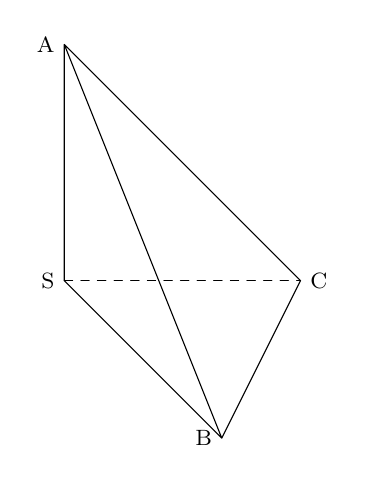
\begin{tikzpicture}[scale=1,font=\footnotesize,line join=round,line cap=round,>=stealth]
					\path 
						 (0,0) coordinate[label=left: S] (S)
						(3,0) coordinate[label=right: C]  (C)
						(2,-2) coordinate[label=left:  B] (B)
						(0,3) coordinate[label=left: A]  (A);
					\draw  (A)--(S)--(B)--(C)--cycle (A)--(B);
					\draw[dashed]  (S)--(C);
				\end{tikzpicture}
		\end{center}
		Ta có $\heva{&SB  \perp SA \\& SC \perp SA}$
		Do đó $\left[B,SA,C\right]=\widehat{CSB}=90^{\circ}$ 
	 }
\end{ex}

% nguồn: Ok_TracNghiemLop11_Lan1
\begin{ex}%[1H8N6-2]%[ma:3c0f22ca]
	Cho hình lăng trụ đứng $ABC.A'B'C'$ có đáy $ABC$  là tam giác vuông tại $A$. Góc phẳng nhị diện $\left[B, AA', C\right]$ có số đo bằng
	 \choice
		{$30^\circ$} 
		 {$45^\circ$}
		{$60^\circ$} 
		{\True $90^\circ$} 
	 \loigiai{ \immini{
		Ta có $BA\perp AA'$ và $CA\perp AA'$ suy ra $\widehat{BAC}$ là góc phẳng nhị diện $\left[B, AA', C\right]$ và bằng  $90^\circ$.}
		{ 
		{ 
		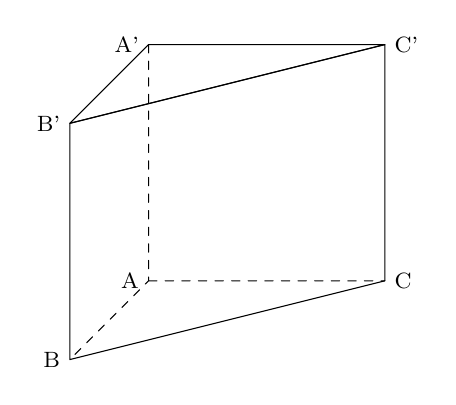
\begin{tikzpicture}[scale=1,font=\footnotesize,line join=round,line cap=round,>=stealth]
				\path 
					(0,3)  coordinate[label=left: A'] (A')
					(0,0) coordinate[label=left: A] (A) 
					(3,0) coordinate[label=right: C] (C) 
					 (3,3) coordinate[label=right: C'] (C')
					(-1,2) coordinate[label=left: B']  (B')
					 (-1,-1) coordinate[label=left: B] (B);
				 \draw (A')--(B')--(C')--cycle;
				\draw (B)--(B')--(C')--(C)--cycle; 
				\draw[dashed] (A')--(A)--(B) 
					(A)--(C); 
			\end{tikzpicture}
		} 
		 }
	 }
\end{ex}

% nguồn: Ok_TracNghiemLop11_Lan1
\begin{ex}%[1H8N6-2]%[ma:daecd959]
	Trong các mệnh đề nào  sau đây đúng?
	\choice 
		{\True Số đo của góc nhị  diện nhận giá trị từ $0^{\circ}$ đến $180^{\circ}$}
		{Số đo  của góc nhị diện nhận giá trị từ $0^{\circ}$ đến $90^{\circ}$}
		{Số đo của góc nhị diện nhận giá  trị từ $90^{\circ}$ đến $180^{\circ}$}
		{Hai mặt phẳng cắt nhau tạo thành hai  góc nhị diện}
	\loigiai{Theo lý thuyết có số đo của góc nhị diện nhận giá trị từ $0^{\circ}$ đến $180^{\circ}$.} 
\end{ex}

% nguồn: Ok_TracNghiemLop11_Lan1
\begin{ex}%[1H8H6-2]%[ma:59ddd0c6]
	Cho hình chóp $S.ABC$ có $\left(SAB\right)$ và $\left(SAC\right)$ cùng vuông góc với đáy. Tam giác $ABC$ vuông tại  B và $M$ là trung điểm của $BC$. Khi đó góc nhị diện $\left[S,BC,A\right]$ là góc nào sau đây?
	\choice 
		{\True $\widehat{SBA}$} 
		 {$\widehat{SMA}$}
		 {$\widehat{SCA}$}
		{$\widehat{ASB}$} 
	\loigiai{ 
		\begin{center}
			\begin{tikzpicture}[scale=1,font=\footnotesize,line join=round,line cap=round,>=stealth]
					\path 
						(0,0)  coordinate[label=left: A] (A)
						(3,0) coordinate[label=right: C]  (C)
						(2,-2) coordinate[label=left: B] (B) 
						(0,3)  coordinate[label=left: S] (S)
						($(B)!.5!(C)$)  coordinate[label=right: M] (M);
					\draw  (S)--(A)--(B)--(C)--cycle (S)--(B);
					\draw[dashed]  (A)--(C)
						(A)--(M); 
				\end{tikzpicture}
		\end{center}
		Ta có $\left(SAB\right)$ và $\left(SAC\right)$ cùng vuông góc với $(ABC)$ nên $SA \perp  (ABC)$
		Lại có $AB \perp  BC$ và $SA \perp BC$ ( Do $SA \perp (ABC)$)
		Suy  ra $\left[S,BC,A\right]=\widehat{SBA}$
	} 
\end{ex}

% nguồn: Ok_TracNghiemLop11_Lan1
\begin{ex}%[1H8H6-2]%[ma:bb2d298c]
	Cho hình lăng trụ đứng $ABC.A'B'C'$ có đáy $ABC$ là tam giác vuông tại $B$, $AB=a\sqrt{3}$, $BC=a$. Góc phẳng nhị  diện $\left[B,AA',C\right]$ có số đo
	 \choice
		{\True $30^\circ$} 
		{$60^\circ$} 
		 {$120^{\circ}$}
		{$90^\circ$} 
	 \loigiai{
		\begin{center}
			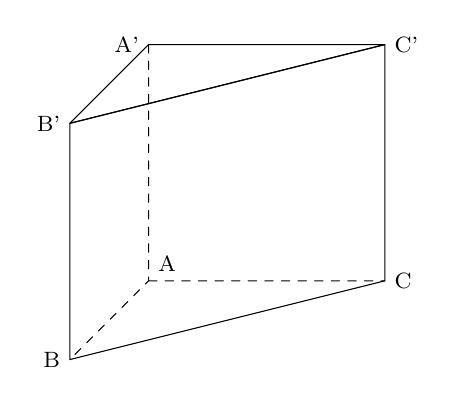
\begin{tikzpicture}[scale=1,font=\footnotesize,line join=round,line cap=round,>=stealth]
					\path 
						(0,3)  coordinate[label=left: A'] (A')
						(0,0) coordinate[label=above right: A]  (A)
						(3,0)  coordinate[label=right: C] (C)
						(3,3)  coordinate[label=right: C'] (C')
						(-1,2)  coordinate[label=left: B'] (B')
						(-1,-1) coordinate[label=left: B]  (B);
					\draw  (A')--(B')--(C')--cycle;
					\draw (B)--(B')--(C')--(C)--cycle; 
					\draw[dashed]  (A')--(A)--(B)
						(A)--(C); 
				\end{tikzpicture}
		\end{center}
		Do $ABC.A'B'C'$ là lăng trụ đứng, nên ta có $\heva{&AC \perp AA' \\ & AB \perp  AA'}$.\\
		Suy  ra $\left[B,AA',C\right]=\widehat{CAB}$.\\
		Xét $\triangle ABC$ vuông tại $B$.\\ 
		 Ta có $\tan CAB =\dfrac{BC}{AB}=\dfrac{a}{a\sqrt{3}}=\dfrac{\sqrt{3}}{3}$.\\
		Vậy $\left[B,AA',C\right]=\widehat{CAB}=30^{\circ}$. 
	 }
\end{ex}

% nguồn: Ok_TracNghiemLop11_Lan1
\begin{ex}%[1H8H6-2]%[ma:376a5452]
	 Cho hình chóp $S.ABC$ có đáy $ABC$ là tam giác vuông cân tại $A$, $SA\perp \left(ABC\right)$. Góc phẳng nhị diện $\left[B, SA, C\right]$ có số đo bằng
	 \choice
		 {$30^\circ$}
		{$45^\circ$} 
		{$60^\circ$} 
		 {\True $90^\circ$}
	 \loigiai{ \immini{
		Ta có $BA\perp SA$ và $CA\perp SA$ suy ra $\widehat{BAC}$ là góc phẳng nhị diện $\left[B, SA, C\right]$ và bằng  $90^\circ$.}
		{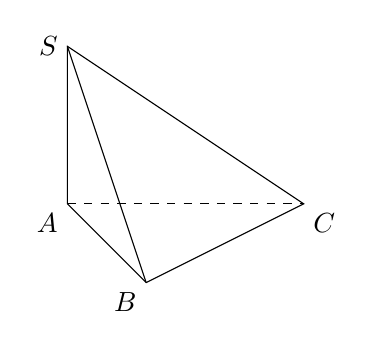
\begin{tikzpicture}
		\draw (0,0)--(1,-1)--(3,0)--(0,2)--cycle; 
		\draw[dashed] (0,0)--(3,0); 
		 \draw (0,2)--(1,-1);
		\node[below left] at (0,0)  {$A$};
		\node[below left]at  (1,-1) {$B$};
		 \node[below right]at (3,0) {$C$};
		 \node[left]at (0,2) {$S$};
	\end{tikzpicture}
		} 
	} 
\end{ex}

% nguồn: Ok_TracNghiemLop11_Lan1
\begin{ex}%[1H8H6-2]%[ma:7d5fb690]
	Cho hình lập phương $MNPQ.M'N'P'Q'$ có cạnh  $a$. Số đo của góc nhị diện $[N,MM',P]$ bằng
	\choice 
		{$30^{\circ}$} 
		{\True $45^{\circ}$} 
		 {$60^{\circ}$}
		{$90^{\circ}$} 
	\loigiai{ 
	 \immini{
		 Số đo của góc nhị diện $[N,MM',P]$ bằng $[N,MM',P]=(NM,PM)=\widehat{NMP}=45^{\circ}$.
		}{ 
		\begin{tikzpicture}[scale=0.7,font=\footnotesize,line join=round,line cap=round,>=stealth]
				\path 
					 (0,0) coordinate (M)
					 (1,0.8) coordinate (Q)
					(4,0) coordinate (N) 
					($(N)+(Q)-(M)$) coordinate (P) 
					($(Q)+(90:3.5)$)  coordinate (Q')
					($(M)-(Q)+(Q')$)  coordinate (M')
					($(N)-(Q)+(Q')$) coordinate  (N')
					($(P)-(Q)+(Q')$) coordinate (P'); 
				\draw  (M')--(M)--(N)--(P)--(P')--(Q')--cycle (M')--(N')--(P')
					 (N)--(N');
				\draw[dashed] (N)--(Q)--(P)--(M) 
					 (Q')--(Q)--(M)
					 (M')--(P);
				\foreach \p/\q in  {Q/160,M/-135,N/-45,P/0,Q'/90,M'/180,N'/-20,P'/0}
				\fill[black] (\p)  node[shift={(\q:3mm)}]{$\p$} circle (1.0pt);
			\end{tikzpicture}
	}} 
\end{ex}

% nguồn: Ok_TracNghiemLop11_Lan1
\begin{ex}%[1H8H6-2]%[ma:a41d5f60]
	Cho hình chóp $S.ABC$ có $SA\perp \left(ABC\right)$. Gọi $H$ là hình chiếu của $A$ trên $BC$. Biết $\triangle ABC$ vuông tại $A$, $\widehat{ABC}=30^{\circ}$, $AC=a$, $SA=\dfrac{a\sqrt{3}}{2}$. Tính số đo góc  nhị diện $\left[S,BC,A\right]$
	 \choice
		{$30^\circ$} 
		 {\True $45^\circ$}
		 {$60^\circ$}
		{$75^\circ$} 
	 \loigiai{\immini{
		 Ta có $SA\perp \left(ABC\right)\Rightarrow SA\perp BC$.\\
		Theo giả  thiết $AH\perp BC$ $\Rightarrow BC\perp \left(SAH\right)$.\\
		$\Rightarrow \left[S,BC,A\right]=\widehat{SHA}$.\\ 
		Vì  tam giác $ABC$ vuông tại $A$.\\
		nên ta có $\tan  \widehat{ABC}=\dfrac{AC}{AB}$ $\Rightarrow AB=\dfrac{AC}{\tan 30^{\circ}}=a\sqrt{3}$.\\
		Khi  đó:
		\begin{align*}
			\dfrac{1}{AH^2}&=\dfrac{1}{AB^2}+\dfrac{1}{AC^2}\\ 
			&=\dfrac{1}{3a^2}+\dfrac{1}{a^2}=\dfrac{4}{3a^2} \\ 
			\Rightarrow  AH&=\dfrac{a\sqrt{3}}{2}.
		\end{align*}
		Tam giác $SAH$  vuông tại $A$ có $SA=AH=\dfrac{a\sqrt{3}}{2}$ $\Rightarrow \widehat{SHA}=45^{\circ}$.}
		 {
		\begin{tikzpicture}
				 \path
					 (0,0) coordinate[label=left: A](A)
					 (3,0) coordinate[label=right: C](C)
					(-2,-2)  coordinate[label=left: B](B)
					(0,4) coordinate[label=above: S](S) 
					($(B)!0.7!(C)$)  coordinate[label=below: H](H);
				\draw  (S)--(B)--(C)--cycle (S)--(H);
				\draw[dashed]  (B)--(A)--(S)
					 (A)--(C)
					(A)--(H); 
			\end{tikzpicture}
		 }
	 }
\end{ex}

% nguồn: Ok_TracNghiemLop11_Lan1
\begin{ex}%[1H8H6-2]%[ma:c2c1750c]
	\immini 
	{ Trong hình bên, máy tính xách tay đang mở gợi nên hình ảnh  của một góc nhị diện. Ta gọi số đo góc nhị diện đó là độ mở của màn hình máy tính. Tính độ mở của màn hình máy tính theo đơn vị độ, biết tam giác $ABC$ có độ dài các cạnh là $AB=AC=30$ cm và $BC=30\sqrt{3}$ cm.
	 \choice
		{$90^\circ$} 
		{$60^\circ$} 
		{$45^\circ$} 
		{\True  $120^\circ$}
		 }
		 {
		\begin{tikzpicture}[scale=0.7,font=\footnotesize,line join=round,line cap=round,>=stealth]
				 \path
					(0,0) coordinate (A) 
					(-1,5) coordinate  (B)
					(3,4) coordinate (D) 
					 (4,1) coordinate (E)
					(3.5,-1)  coordinate (C)
					(7,0.2) coordinate (F) 
					($(A)+(0.5,0)$)  coordinate (A')
					($(A)!10/11!(E)$) coordinate  (M)
					($(M)+(0.5,0)$) coordinate  (M')
					($(A)!1/2!(C)$)  coordinate (N)
					 ($(N)+(0.5,0)$) coordinate (N')
					($(E)!0.65!(F)$) coordinate (O) 
					 ($(O)-(0.3,0)$) coordinate (O');
				\draw[blue!50,line  width=2pt] (A)--(C)--(F);
				\draw[blue!70,line  width=3pt] (A)--(B)--(D)--(E)--(A);
				\fill[blue!30]  (O')--(N')--(A')--(M')--cycle;
				\draw (F)--(E) 
					(B)--(C); 
				\foreach \x/\g in {A/160,B/180,C/270} \fill[black] (\x) circle (1pt)+(\g:0.6)  node{$\x$};
			\end{tikzpicture}
		 }
	 \loigiai{
		Góc  nhị diện đã cho có số đo bằng số đo của góc $\widehat{BAC}$.\\
		Trong tam giác $ABC$ ta có $\cos \widehat{BAC}=\dfrac{AB^2+AC^2-BC^2}{2\cdot AB \cdot AC}=\dfrac{30^2+30^2-\left(30\sqrt{3}\right)^2}{2\cdot  30 \cdot 30}=-\dfrac{1}{2}\Rightarrow \widehat{BAC}=120^\circ$.\\
		Vậy độ mở của màn hình  máy tính là $120^\circ$.
	 }
\end{ex}

% nguồn: Ok_TracNghiemLop11_Lan1
\begin{ex}%[1H8V6-2]%[ma:6f2ee9de]
	Cho hình chóp  $S.ABCD$ có đáy $ABCD$ là hình thoi cạnh $a$ tâm $O$, $SO\perp \left(ABCD\right)$, $SO=\dfrac{a\sqrt{6}}{3}, OB=\dfrac{a\sqrt{3}}{3}$. Góc phẳng nhị diện $\left[A, BC, S\right]$ có số đo bằng
	\choice 
		 {$30^\circ$}
		{$45^\circ$} 
		{\True $60^\circ$} 
		{$90^\circ$} 
	\loigiai{\immini{ 
		Gọi $H$ là hình chiếu của $S$ lên $BC$. 
		Ta có $SH\perp BC$ và $OH\perp BC$ suy ra $\widehat{SHO}$ là góc phẳng nhị diện $\left[A, BC, S\right]$. 
		Ta có $OC=\sqrt{BC^2-OB^2}=\dfrac{a\sqrt{6}}{3}$ 
		$\dfrac{1}{OH^2}=\dfrac{1}{OB^2}+\dfrac{1}{OC^2} \Rightarrow  OH=\dfrac{a\sqrt{2}}{3}$.
		Trong tam giác vuông $SHO$  ta có
		$\tan SHO=\dfrac{SO}{OH}=\sqrt{3}$. 
		 Suy ra $\widehat{SHO}=60^{\circ}$.}
		{ 
		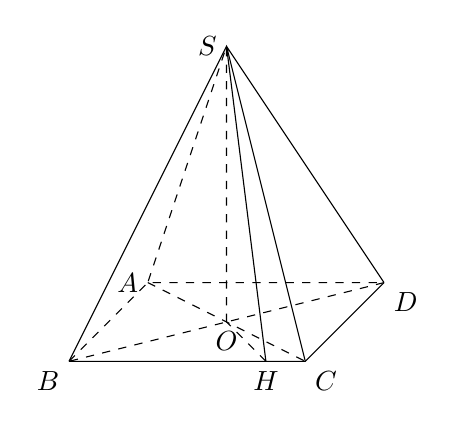
\begin{tikzpicture}
				\draw  (3,0)--(2,-1)--(-1,-1);
				\draw[dashed]  (-1,-1)--(0,0)--(3,0);
				\draw[dashed] (0,0)--(2,-1) 
					 (3,0)--(-1,-1);
				 \draw[dashed] (1,-.5)--(1,3)--(0,0);
				\draw (-1,-1)--(1,3)--(2,-1) 
					(3,0)--(1,3); 
				\draw (1,3)--(1.5,-1); 
				\draw[dashed] (1.5,-1)--(1,-.5); 
				\node[left] at  (0,0) {$A$};
				\node[below left]at  (-1,-1) {$B$};
				\node[below  right]at (3,0) {$D$};
				\node[below right]at (2,-1)  {$C$};
				\node[left]at  (1,3) {$S$};
				\node[below]at  (1,-.5) {$O$};
				\node[below] at (1.5,-1)  {$H$};
			\end{tikzpicture}
		 }
	 }
\end{ex}


%%%%%%%%%%%%%%%% ĐÚNG/SAI %%%%%%%%%%%%%%%%

% nguồn: Ok_dungsai_lop11_Lan1
\begin{ex}%[1H8N6-2]%[ma:de7e191a]
 Cho hai mặt phẳng $(P)$ và $(Q)$ cắt nhau  theo giao tuyến $a$.
 \choiceTF 
  {\True Nếu $(P)$ và $(Q)$ cùng vuông góc với mặt phẳng $(R)$ thì $a$ cũng vuông góc  với $(R)$}
  {\True Góc giữa  hai mặt phẳng $(P)$ và $(Q)$ là góc giữa hai đường thẳng lần lượt vuông góc với $(P)$ và $(Q)$}
  {Hai mặt phẳng cắt nhau tạo thành hai góc  nhị diện}
  {\True Số đo của góc nhị diện có thể lớn hơn $90^{\circ}$} 
  \loigiai{
  \begin{itemchoice}
    \itemch Đúng. Theo định lí hai mặt phẳng vuông góc.
   \itemch Đúng. Theo định nghĩa góc giữa hai mặt  phẳng.
   \itemch Sai. Hai mặt phẳng cắt  nhau tạo thành bốn góc nhị diện.
   \itemch Đúng. Số đo của góc  nhị diện có thể nhận giá trị từ $0^{\circ}$ đến $180^{\circ}$.
  \end{itemchoice}
  }
\end{ex}

% nguồn: Ok_dungsai_lop11_Lan1
\begin{ex}%[1H8H6-2]%[ma:27fa65b7]
 Cho hình chóp tứ giác đều có cạnh đáy bằng $a$, chiều cao bằng $\dfrac{a}{2}$. Gọi $M$ là trung điểm $CD$  như hình vẽ.
 \begin{center}
  \begin{tikzpicture}[scale=0.7]
    \path 
     (0:0) coordinate (A) 
     +(0:5)  coordinate (D)
      +(-140:2.5) coordinate (B)
     ($(B)+(D)-(A)$) coordinate  (C)
     (intersection of A--C and B--D)  coordinate (O)
     ++(90:4) coordinate  (S);
    \path (S)--(O) node[right,midway]{$\dfrac{a}{2}$}; 
    \path  (B)--(C) node[below,midway]{$a$};
    \path ($(D)!.5!(C)$) coordinate  (M);
    \draw[thin]  pic[teal,draw,angle radius = 12pt]{angle = S--M--O};
    \foreach \x/\y/\z in {S/O/D,S/M/D,O/M/C}{ 
     \draw pic[red,draw,angle radius = 6pt]{right angle  = \x--\y--\z};}
    \draw[dashed] 
     (A)--(B) 
      (A)--(D)
      (A)--(S)
     (A)--(C) 
     (B)--(D) 
     (S)--(O)--(M); 
     \draw
     (D)--(C)--(B) 
     (S)--(B) 
     (S)--(C) 
     (M)--(S)--(D); 
     \foreach \x/\g in {A/135,D/0,C/-45,B/-135,O/-90,S/90,M/-45}
     \fill [blue] (\x) circle (1pt)
     +(\g:3mm) node {$\x$}; 
   \end{tikzpicture}
 \end{center}
  \choiceTF
  {Đường thẳng $SD$ là  cạnh của nhị diện $(SAD)$ và $(SCD)$}
  {Góc nhị diện $[(SAC), AC,(ABCD)]$ là góc nhị diện vuông} 
  {Góc  $\widehat{SDO}$ là góc phẳng nhị diện $[S, CD, O]$}
   {Số đo góc phẳng nhị diện $[S, CD, O]$ bằng $45^{\circ}$}
 \loigiai{ 
  \begin{itemchoice}
   \itemch $\heva{&S\in(SAD) \cap(SCD) \\  &D\in(SAD) \cap(SCD)} \Rightarrow(SAD) \cap(SCD)=SD$.\\
   Vậy $SD$ là cạnh của nhị diện $(SAD)$ và  $(SCD)$.
   \itemch Ta có: $\heva{&(SAC) \cap(ABCD)=AC\\&SO\perp  AC\\&DO\perp AC} \Rightarrow[(SAC), AC,(ABCD)]=[S, AC, O]=\widehat{SOD}=90^{\circ}$.
   \itemch Ta có: $\heva{&SM\perp CD\\ &OM\perp CD} \Rightarrow[S,  CD, O]=\widehat{SMO}$.
   \itemch Ta có: $\heva{&SM\perp CD\\ &OM\perp CD} \Rightarrow[S,  CD, O]=\widehat{SMO}$.\\
   Xét $\triangle SOM$  vuông tại $O$ có: $\tan \widehat{SMO}=\dfrac{SO}{OM} \Rightarrow \tan \widehat{SMO}=1\Rightarrow \widehat{SMO}=45^{\circ}$.
  \end{itemchoice}
  }
\end{ex}

% nguồn: Ok_dungsai_lop11_Lan1
\begin{ex}%[1H8H6-2]%[ma:706ddc54]
 Cho hình  chóp $S.ABCD$ có $SA\perp \left(ABCD\right)$, $ABCD$ là hình thoi cạnh $a$, $AC=a$, $SA=\dfrac{a}{2}$.
  \choiceTF
  {\True $BD\perp\left(SAC\right)$} 
  {$SD\perp  AB$}
  {\True Góc  giữa $SD$ và $\left(ABCD\right)$ nhỏ hơn $30^\circ$}
  {\True  Số đo của góc nhị diện $\left[S,CD,A\right]$ bằng $30^\circ$}
 \loigiai{ 
  \begin{center}
   \begin{tikzpicture}[line join=round,line cap=round,thick,scale=0.8]
      \coordinate (A) at (0,0);
     \coordinate (B) at (-2,-3); 
     \coordinate (D) at (5,0); 
      \coordinate (C) at ($(B)+(D)-(A)$);
      \coordinate (S) at ($(A)+(0,5)$);
     \coordinate (H) at ($(C)!0.5!(D)$); 
     \draw[name  path=AC,dashed] (A)--(C);
     \draw[name  path=BH,dashed] (B)--(H);
      \draw pic[draw,angle radius=3mm,thin]{right angle=D--H--S};
      \path (A)--(B) node [rotate=0,above left,sloped,pos=0.5] {$a$};
     \path (A)--(C) node  [rotate=0,above,sloped,pos=0.5] {$a$};
     \path (S)--(A) node [rotate=90,right,sloped,pos=0.5]  {$\dfrac{a}{2}$};
      \draw[name path=SH] (S)--(H);
     \draw (S)--(B) 
       (S)--(C)
       (S)--(D)
       (B)--(C)--(D);
     \draw[dashed](S)--(A) 
      (A)--(B) 
      (A)--(D); 
     \pic[draw,thin,angle radius=3mm] {right  angle = S--A--D} pic[draw,thin,angle radius=3mm] {right angle = S--A--B};
      \foreach \i/\g in {S/90,A/-90,B/-90,C/-90,D/0,H/0}{\draw[fill=black](\i) circle (0pt)
       ($(\i)+(\g:3mm)$) node[scale=1]{$\i$};}
    \end{tikzpicture}
  \end{center}
  \begin{itemchoice}
   \itemch Có $BD\perp AC$ (do $ABCD$  là hình thoi) và $BD\perp SA$ (do $SA\perp (ABCD)$).\\ Nên $BD\perp\left(SAC\right)$.
   \itemch $\left(AB,SD\right)=\left(CD,SD\right)$. Có\\  $SD=\sqrt{S{A^2}+A{D^2}}=\sqrt{\left(\dfrac{a}{2}\right)^2+a^2}=\dfrac{\sqrt 5a}{2}$.\\ $SC=\sqrt{S{A^2}+A{C^2}}=\sqrt{\left(\dfrac{a}{2}\right)^2+a^2}=\dfrac{\sqrt 5 a}{2}$ và $CD=a$.
    $SD$ không vuông góc $CD$ do không thỏa định lí Pytago đảo.
   \itemch  Hình chiếu của $SD$ lên $\left(ABCD\right)$ là $AD$, do đó góc giữa $SD$ và $\left(ABCD\right)$ là góc giữa $SD$ và $AD$, chính là góc $\widehat{SDA}$. Ta có
   $\tan\widehat{SDA}=\dfrac{SA}{AD}=\dfrac{\dfrac{a}{2}}{a}=\dfrac{1}{2}\Rightarrow\widehat{SDA}\approx 26{,}5^\circ$. 
   \itemch Gọi $H$ là hình chiếu của $A$  trên $CD$. Khi đó, $AH\perp CD$.\\
    Vì $SA\perp (ABCD)$ nên $SA\perp CD$. Suy ra $CD\perp (SAH)$.\\
   Khi đó, $SH\perp CD$. Như vậy, số đo của $\left[S,CD,A\right]$ bằng $\widehat{SHA}$.\\ 
    Ta có $AH=\dfrac{a\sqrt3}{2},SA=\dfrac{a}{2}$ nên $\tan\widehat{SHA}=\dfrac{SA}{AH}=\dfrac{\dfrac{a}{2}}{\dfrac{a\sqrt 3}{2}}=\dfrac{\sqrt 3}{3}$.\\
   Vậy số đo của góc nhị diện  $\left[S,CD,A\right]$ bằng $\widehat{SHA}=30^\circ$.
  \end{itemchoice}
 } 
\end{ex}

% nguồn: Ok_dungsai_lop11_Lan2
\begin{ex}%[1H8H6-2]%[ma:a6b97e74]
	Cho hình chóp $S.ABCD$, đáy $ABCD$ là hình thoi tâm $O$ cạnh $a$, góc $\widehat{ABC}=60^\circ$. Tam giác $SAC$ đều, tam giác $SBD$ cân tại ${S}$.  (đơn vị độ, kết quả làm tròn đến hàng đơn vị)
	\choiceTF 
		{\True  $(SAC) \perp (ABCD)$}
		 {$\left( (SBD),(ABCD) \right)=60^\circ$}
		 {$SO=\dfrac{a\sqrt{3}}{3}$}
		 {$\left((SCD),(ABCD)\right) \approx 60^\circ$}
	 \loigiai{
		\begin{center}
			\begin{tikzpicture}[line join=round,line cap=round,scale=1]
					\path 
						(0,0) coordinate (A) 
						(-2,-1.5)  coordinate (B)
						(3,-1.5) coordinate (C) 
						($(A)+(C)-(B)$) coordinate (D) 
						 ($(B)!0.5!(D)$) coordinate (O)
						 ($(O)+(0,4)$) coordinate (S)
						($(C)!0.3!(D)$) coordinate  (M);
					\draw  (S)--(B)--(C)--(D)--(S)--(C)
						 (S)--(M);
					\draw[dashed,thin] (C)--(A)--(S)--(O) 
						(A)--(B)--(D)--(A) 
						(O)--(M); 
					\pic[draw,thin,angle radius=2mm] {right  angle = S--O--D}
						pic[draw,thin,angle  radius=2mm] {right angle = B--O--C}
						pic[draw,thin,angle radius=2mm] {right angle =  O--M--C};
					\foreach \i/\g  in {S/90,A/170,B/-90,C/-90,D/-60,O/-80,M/-30}{\fill (\i) circle (1pt)
						 ($(\i)+(\g:3mm)$) node[scale=1]{$\i$};}
				\end{tikzpicture}
		\end{center}
		\begin{itemchoice}
			\itemch Tam giác $SAC$ đều có $O$ là trung điểm $AC$ nên $SO \perp AC$  \quad (1).\\
			Tam giác $SBD$ cân tại $S$ có $O$ là trung điểm $BD$ nên $SO  \perp BD$ \quad (2).\\
			Từ  (1) và (2) suy ra $SO \perp (ABCD)$.\\
			Mặt khác $SO \subset (SAC)$ nên $(SAC) \perp (ABCD)$. 
			\itemch Các  tam giác $ABC$, $ACD$ lần lượt cân tại $B$ và $D$ mà $\widehat{ABC}=\widehat{ADC}=60^\circ$ nên hai tam giác $ABC$, $ACD$ đều cạnh $a$.\\
			Kẻ  đường cao $OM$ của tam giác $OCD$.\\
			Ta có $\heva{& CD \perp OM \\ &  CD \perp SO} \Rightarrow CD \perp (SOM) \Rightarrow CD \perp SM$.\\
			Khi đó $\heva{& (SCD)\cap  (ABCD)=CD \\ & OM \perp CD, SM \perp CD \\ & OM \subset (ABCD), SM \subset (SCD)} \Rightarrow \left((SCD),(ABCD)\right)=(SM,OM)=\widehat{SMO}$.\\
			 Tam giác $SAC$ đều nên $SO = \dfrac{AC \sqrt{3}}{2}=\dfrac{a \sqrt{3}}{2}$.
			\itemch  Ta có $OC=\dfrac{AC}{2}=\dfrac{a}{2}$, $OD=\dfrac{a \sqrt{3}}{2}$.\\
			Tam giác  $OCD$ vuông tại $O$, đường cao $OM$ nên
			 $$\dfrac{1}{OM^2}=\dfrac{1}{OC^2}+\dfrac{1}{OD^2} \Rightarrow OM = \dfrac{OC \cdot OD}{\sqrt{OC^2+OD^2}}=\dfrac{a \sqrt{3}}{4}.$$
			Tam giác $SOM$ vuông tại $O$ có 
			$$\tan  \widehat{SMO}=\dfrac{SO}{OM}=\dfrac{\dfrac{a \sqrt{3}}{2}}{\dfrac{a \sqrt{3}}{4}}=2 \Rightarrow \widehat{SMO} \approx 63{,}43^{\circ}.$$
			Vậy $\left((SCD),(ABCD)\right)=\widehat{SMO} \approx 63^\circ$. 
		\end{itemchoice}
	 }
\end{ex}

% nguồn: Ok_dungsai_lop11_Lan2
\begin{ex}%[1H8H6-2]%[ma:bc2ba151]
	Cho hình chóp $S.ABCD$ có $SA$ vuông góc với mặt phẳng $(ABCD)$, $SA=a \sqrt{2}$, $ABCD$ là hình thang vuông tại  $A$ và $D$ với $AB=2a$, $AD=DC=a$.
	\choiceTF 
		{\True  $BC \perp SC$}
		 {$\left((SBC),(ABC)\right)=30^\circ$}
		{$BC=a\sqrt{3}$} 
		{\True  $\left((SBC),(SAB)\right)=60^\circ$}
	\loigiai{ 
		\begin{center}
			\begin{tikzpicture}[line join=round,line cap=round,scale=1]
					 \path
						(0,0) coordinate (A) 
						(-2,-1.5) coordinate (D) 
						(1,-1.5)  coordinate (C)
						(6,0) coordinate  (B)
						($(B)!0.5!(A)$)  coordinate (M)
						(0,3) coordinate (S) 
						($(S)!0.6!(B)$)  coordinate (N);
					 \draw (S)--(B)--(C)--(D)--(S)--(C)
						 (C)--(N);
					\draw[dashed,thin] (S)--(A)--(C)--(M)--(N) 
						(D)--(A)--(B); 
					\pic[draw,thin,angle radius=2mm] {right angle = S--A--D} 
						pic[draw,thin,angle radius=2mm] {right angle = M--N--B}; 
					\foreach \i/\g in {S/90,A/45,B/-60,C/-90,D/-90,M/-60,N/70}{\fill (\i) circle  (1pt)
						($(\i)+(\g:3mm)$) node[scale=1]{$\i$};} 
				\end{tikzpicture}
		\end{center}
		\begin{itemchoice}
			 \itemch Gọi $M$ là trung điểm $AB$, khi đó $AMCD$ là hình vuông, đường chéo $AC=a \sqrt{2}$.\\
			Tam giác $ACB$ có trung tuyến $CM$ thoả mãn $CM=\dfrac{AB}{2}$ nên $ACB$ là tam giác vuông tại $C$.\\ 
			Ta có $\heva{& AC \perp BC \\ & SA \perp BC~(\text{do } SA \perp  (ABCD))} \Rightarrow BC \perp (SAC) \Rightarrow BC \perp SC$.
			\itemch Ta có $\heva{& (SBC) \cap (ABC) = BC \\ & AC \perp BC, SC \perp BC \\ & AC \subset (ABC), SC  \subset (SBC)} \Rightarrow \left((S B C),(A B C)\right)=(SC, AC) = \widehat{SCA}$.\\
			Tam  giác $SAC$ vuông tại $A$ có
			$$\tan  \widehat{SCA} = \dfrac{SA}{AC} = \dfrac{a \sqrt{2}}{a \sqrt{2}}=1 \Rightarrow \widehat{SCA}=45^{\circ}.$$
			Vậy $\left((SBC),(ABC)\right) = \widehat{SCA} = 45^{\circ}$. 
			\itemch Trong tam giác $SAB$, kẻ $MN$ vuông góc với $SB$ tại $N$.\\ 
			Ta có $\heva{& CM \perp AB \\ & CM \perp SA} \Rightarrow CM \perp (SAB) \Rightarrow CM \perp  SB$.\\
			 Vì $\heva{& SB \perp CM \\ & SB \perp MN} \Rightarrow SB \perp (CMN) \Rightarrow SB \perp CN$.\\
			Khi đó $\heva{& (SB) \cap (SAB) = SB \\ & CN  \perp SB, MN \perp SB \\ & CN \subset (SBC), MN \subset (SAB)} \Rightarrow \left((SBC),(SAB)\right)=(CN, MN)=\widehat{CNM}$.\\
			Ta  có $SC=\sqrt{SA^2+AC^2}=2a$, $BC=\sqrt{BM^2+CM^2}=a \sqrt{2}$.
			\itemch Tam giác $SBC$  vuông tại $C$ có
			$$\dfrac{1}{CN^2} = \dfrac{1}{SC^2}+\dfrac{1}{BC^2}  \Rightarrow CN= \dfrac{2 a \sqrt{3}}{3}.$$
			 Tam giác $CMN$ vuông tại $M$ có
			$$\sin \widehat{CNM}=\dfrac{CM}{CN}=\dfrac{\sqrt{3}}{2}  \Rightarrow \widehat{CNM}=60^{\circ}.$$
			Vậy $\left((SBC),(SAB)\right)  = \widehat{CNM}=60^{\circ}$.
		\end{itemchoice}
	} 
\end{ex}

% nguồn: Ok_dungsai_lop11_Lan2
\begin{ex}%[1H8H6-2]%[ma:fa673873]
	Cho hình chóp $S.ABC$ có cạnh bên $SA$ vuông góc với mặt phẳng đáy, tam giác $ABC$ vuông  cân tại $B$. Biết $SB=a\sqrt{3}$, $AB=a$.
	 \choiceTF
		{\True  $SA=a\sqrt{2}$}
		{\True Tang  góc giữa $SB$ và mặt phẳng $(ABC)$ bằng $\sqrt{2}$}
		{Sin góc giữa $SB$  và mặt phẳng $(SAC)$ bằng $\dfrac{\sqrt{6}}{8}$}
		{\True Số đo góc phẳng nhị diện $\left[S,BC,A\right]$ bằng $55^\circ$ (đơn vị độ, kết quả làm tròn đến  hàng đơn vị)}
	 \loigiai{
		\begin{center}
			\begin{tikzpicture}[line join=round,line cap=round,scale=1]
					 \path
						(0,0) coordinate (A) 
						(1.5,-1.5) coordinate  (B)
						(5,0) coordinate (C) 
						(0,3.5)  coordinate (S)
						($(A)!1/2!(C)$) coordinate (H); 
					\draw (S)--(A)--(B)  node[pos=0.5,rotate=0,below,scale=0.8]{$a$}--(C) node[pos=0.5,rotate=0,below,scale=0.8]{$a$}--(S)--(B) node[pos=0.5,rotate=110,above,scale=0.8]{$a\sqrt{3}$};
					 \draw[dashed,thin] (S)--(H)--(B)
						(A)--(C); 
					\pic[draw,thin,angle radius=2mm] {right angle =  S--A--C}
						pic[draw,thin,angle  radius=2mm] {right angle = A--B--C}
						pic[draw,thin,angle radius=2mm]  {right angle = B--H--A};
					\foreach \i/\g  in {S/90,A/-130,B/-90,C/-70,H/-50}{\fill (\i) circle (1pt)
						($(\i)+(\g:3mm)$)  node[scale=1]{$\i$};}
				\end{tikzpicture}
		\end{center}
		\begin{itemchoice}
			\itemch Ta có $SA \perp (ABC)$ nên $AB$ là hình chiếu của $SB$  trên mặt phẳng $(ABC)$.\\
			 Suy ra $\left(SB,(ABC)\right)=(SB,AB)=\widehat{SBA}$.\\
			Tam giác $SAB$  vuông tại $A$ có
			$$SA=\sqrt{SB^2-AB^2}=\sqrt{3a^2-a^2}=a\sqrt{2}.$$ 
			\itemch  Tam giác $SAB$ vuông tại $A$ có $\tan \widehat{SBA}=\dfrac{SA}{AB}=\dfrac{a\sqrt{2}}{a}=\sqrt{2}$.\\
			Do đó, tang góc  giữa $SB$ và mặt phẳng $(ABC)$ bằng $\sqrt{2}$.
			\itemch Gọi $H$  là trung điểm $AC$ thì $BH \perp AC$ (do tam giác $ABC$ cân tại $B$).\quad (1)\\
			Ta  lại có $SA \perp (ABC) \Rightarrow BH \perp SA$. \quad (2)\\
			Từ (1) và (2) suy ra $BH \perp (SAC)$ hay $SH$ là  hình chiếu của $SB$ trên mặt phẳng $(SAC)$.\\
			 Vậy $\left(SB,(SAC)\right)=(SB,SH)=\widehat{BSH}$.\\
			 Ta có $BH=\dfrac{a\sqrt{2}}{2}$, suy ra $\sin \widehat{BSH}=\dfrac{BH}{SB}=\dfrac{\dfrac{a\sqrt{2}}{2}}{a\sqrt{3}}=\dfrac{\sqrt{6}}{6}$.
			\itemch Ta có $\heva{& BC \perp AB \\ & BC \perp SA~(\text{do } SA \perp (ABC))} \Rightarrow BC \perp (SAB) \Rightarrow  BC \perp SB$.\\
			Vì vậy $(SB,AB)=\widehat{SBA}$ là góc phẳng nhị diện $\left[S, BC, A\right]$ với $\tan  \widehat{SBA}=\sqrt{2}$ (theo câu a)).\\
			Suy ra $\widehat{SBA}  \approx 55^{\circ}$.
		\end{itemchoice}
	} 
\end{ex}

% nguồn: Ok_dungsai_lop11_Lan2
\begin{ex}%[1H8H6-2]%[ma:8b5b7e57]
	Cho hình chóp $S.ABCD$ có đáy là hình chữ nhật,  $SA\perp(ABCD)$, $SA=AB=2AD$.
	\choiceTF 
		{\True Góc giữa hai mặt phẳng ($SAD$)  và ($SBC$)bằng $45^{\circ}$}
		{\True  Góc giữa hai mặt phẳng $(SAC)$ và $(ABCD)$ bằng $90^{\circ}$}
		{\True Góc giữa  hai mặt phẳng $(SCD)$ và $(SAD)$ bằng $90^{\circ}$}
		{\True Góc giữa hai mặt phẳng $(SCD)$ và $(ABCD)$ là $\widehat{SDA}$} 
	\loigiai{ 
		\begin{center}
			\begin{tikzpicture}[>=stealth,line join=round,line cap=round,font=\footnotesize,scale=.9]
					\path 
						 (0,0) coordinate (A)
						(4,0) coordinate (D) 
						(-130:2.5) coordinate  (B)
						($(B)+(D)-(A)$)  coordinate (C)
						($(A)+(90:4)$) coordinate (S); 
					 \draw (S)--(B)--(C)--(D)--cycle (S)--(C)
						 (S)--++(180:.5)
						(S)--++(0:4)  node[above]{$x$};
					\draw[dashed] (S)--(A)--(D) 
						 (A)--(B);
					\foreach \i/\j  in {A/180,B/-90,C/-90,D/0,S/90}
					\fill[black] (\i)  circle (1pt)
						(\i)  node[shift={(\j:2.5mm)}]{$\i$};
				\end{tikzpicture}
		\end{center}
		\begin{itemchoice}
			\itemch 
			Giao tuyến của hai mặt phẳng $(SAD)$ và $(SBC)$ là đường thẳng $Sx \parallel  AD\parallel BC$.\\
			$\heva{&B C \perp  B A \\
			&B C \perp S A}\Rightarrow B C \perp (SAB) \Rightarrow B C \perp S B$ và  $\heva{&S A \perp A D \\
			 &A D \parallel S x}\Rightarrow SA \perp Sx$.\\
			$\Rightarrow((SAD),(SBC))=(SA, SB)=\widehat{B  S A}$.\\
			Tam giác $SAB$ vuông  tại $A$ và $SA=AB\Rightarrow \triangle SAB$ vuông cân tại $A\Rightarrow \widehat{BSA}=45^{\circ}$.
			\itemch  Ta có $SA\perp(ABCD) \Rightarrow(SAC) \perp(ABCD)$.
			\itemch Ta  có $CD\perp(SAB) \Rightarrow(SCD) \perp(SAB)$.
			\itemch Ta có $CD\perp AD$ và $CD\perp  SD$ nên góc giữa hai mặt phẳng ($SCD$) và $(ABCD)$ là $\widehat{SDA}$.
		\end{itemchoice}
	 }
\end{ex}

% nguồn: Ok_dungsai_lop11_Lan2
\begin{ex}%[1H8H6-2]%[ma:5820d93e]
	Cho hình chóp tam giác  đều $S.ABC$ có cạnh đáy bằng $a$ và cạnh bên bằng $a \sqrt{\dfrac{5}{12}}$. Gọi $O$ là tâm của mặt đáy.
	\choiceTF 
		{Số đo của các góc nhị diện $[S, AB, C]$, $[S,  BC, A]$, $[S, CA, B]$ bằng nhau}
		{Số đo của góc  nhị diện $[S, BC, A]$ bằng số đo của góc giữa hai mặt phẳng $(SBC)$ và $(ABC$}
		{Số đo của góc nhị diện $[S, BC, A]$ bé hơn số đo của góc  $\widehat{SAO}$}
		 {Số đo của góc nhị diện $[S, BC, A]$ bằng $45^{\circ}$}
	\loigiai{ 
		\begin{center}
			\begin{tikzpicture}[scale=0.8,font=\footnotesize,line join=round,line cap=round,>=stealth]
					\path 
						 (0,0) coordinate (A)
						++(-50:2.5)  coordinate (B)
						(5,0) coordinate  (C)
						 (barycentric cs:A=1,B=1,C=1) coordinate (H)
						($(B)!1/2!(C)$) coordinate (M) 
						($(A)!2/3!(M)$) coordinate (O) 
						($(H)+(0,3)$) coordinate  (S);
					\foreach \i in{A,B,C}{\draw  (S)--(\i);};
					 \draw (A)--(B)--(C);
					\draw[dashed]  (A)--(C)
						 (S)--(O)
						(A)--(O); 
					 \foreach \i/\g in {A/180,B/-90,C/0,S/90,O/-90}
					 \fill[black] (\i) circle (1pt)+(\g:4mm) node[scale=1]{$\i$};
					\draw pic[draw,angle radius=2mm]{right angle=S--O--A}; 
				\end{tikzpicture}
		\end{center}
		\begin{itemchoice}
			\itemch Vì $S.ABC$ là hình  chóp tam giác đều nên số đo của các góc nhị diện $[S, A B, C]$, $[S, B C, A]$, $[S, C A, B]$ bằng nhau.
			\itemch Gọi $H$ là giao điểm của $A O$ và $B C$. Vì $\triangle A B C$ đều và $\triangle S B C$ cân tại $S$  nên $H A$ và $H S$ vuông góc với $B C$.\\
			Suy ra $\widehat{A H S}$ là một góc phẳng của góc nhị diện $[S, B C, A]$ và góc giữa hai mặt phẳng $(S B C)$  và $(A B C)$ bằng góc giữa hai đường thẳng $H A$ và $H S$.\\
			Mặt khác, $\widehat{A H S}$ là góc nhọn  nên góc giữa hai mặt phẳng ($S B C$) và ($A B C$) bằng góc $\widehat{A H S}$.
			Vậy số đo của góc nhị diện $[S, B  C, A]$ bằng số đo của góc giữa ($S B C$) và ($A B C$).
			\itemch Vì $O A>O H$ nên $S A>S H$. Do đó  $\widehat{A H S}>\widehat{S A O}$.\\
			Vậy số đo  của góc nhị diện $[S, B C, A]$ lớn hơn số đo của góc $\widehat{S A O}$.
			\itemch $\triangle A B C$ đều có cạnh  bằng $a$ và $H$ là trung điểm của $B C$ nên $A H=\dfrac{a \sqrt{3}}{2}$.\\
			$\triangle S A O$ vuông tại $O$ và có $S A=a \sqrt{\dfrac{5}{12}}, A O=\dfrac{2}{3} A H=\dfrac{a \sqrt{3}}{3}$ nên $$S O=\sqrt{S A^2-A  O^2}=\sqrt{\left(a \sqrt{\dfrac{5}{12}}\right)^2-\left(\dfrac{a \sqrt{3}}{3}\right)^2}=\dfrac{a \sqrt{3}}{6}.$$
			$\triangle S H O$ vuông tại $O$ và lại có $O H=\dfrac{1}{3} A H=\dfrac{a \sqrt{3}}{6}$  nên vuông cân tại $O$. Suy ra $\widehat{A H S}=45^{\circ}$.\\
			 Vậy số đo của góc nhị diện $[S, B C, A]$ bằng $45^{\circ}$.
		\end{itemchoice}
	 }
\end{ex}

% nguồn: Ok_dungsai_lop11_Lan2
\begin{ex}%[1H8H6-2]%[ma:adb97394]
	Cho hình lập phương $ABCD.A' B' C' D'$ có cạnh bằng  $a$. Xét tính đúng sai của các mệnh đề sau
	 \choiceTF
		{Số đo của hai góc nhị diện $\left[A, BD, A'\right]$ và $\left[C, BD, A'\right]$ phụ nhau} 
		{\True Số đo của hai góc nhị diện $\left[A, BD, A'\right]$  và $\left[B', BD, A'\right]$ phụ nhau}
		{Số đo của  góc nhị diện $\left[A, BD, A'\right]$ bằng $30^{\circ}$}
		{Số đo của góc  nhị diện $\left[C', BD, A'\right]$ bằng $60^{\circ}$}
	 \loigiai{
		\begin{center}
			\begin{tikzpicture}[scale=0.8,font=\footnotesize,line join=round,line cap=round,>=stealth]
					\path 
						(0,0) coordinate  (A)
						++(-150:3)  coordinate (B)
						++(0:5) coordinate  (C)
						 ($(A)+(C)-(B)$) coordinate (D);
					\foreach \i in {A,B,C,D}{ 
						\coordinate  (\i') at ($(\i)+(0,4)$);
					 }
					 \draw (A')--(B')--(C')--(D')--cycle;
					 \draw (B)--(B')
						(C)--(C') 
						 (D)--(D')
						(B)--(C)--(D); 
					 \draw[dashed,thin](B)--(A)--(A')
						(A)--(D) 
						(A')--(D) 
						 (A')--(B);
					\foreach \i/\g in  {A'/90,B'/90,C'/90,D'/90,A/-90,B/-90,C/-90,D/-90}
					 \fill[black] (\i) circle (1pt)+(\g:3mm) node[scale=1]{$\i$};
				\end{tikzpicture}
		\end{center}
		\begin{itemchoice}
			\itemch Vì $A C$, $B D$ đồng phẳng và $A$, $C$ ở hai phía khác nhau so với $B D$  nên số đo của hai góc nhị diện $\left[A, B D, A'\right]$ và $\left[C, B D, A'\right]$ bù nhau.
			\itemch Vì $(A B D) \perp\left(B' B D\right)$ nên $\left[A, B D, B'\right]$ là  góc nhị diện vuông.\\
			Mặt khác $A'$ nằm trong góc nhị diện $\left[A, B D, B'\right]$ nên số đo của hai góc nhị diện $\left[A, B D, A'\right]$ và $\left[B',  B D, A'\right]$ phụ nhau.
			\itemch Gọi $O$ là tâm của hình vuông $A B C D$. Khi đó $\widehat{A O A'}$ là góc phẳng của góc nhị  diện $\left[A, B D, A'\right]$.\\
			$\triangle A O A'$ vuông tại $A$ và có $A O=\dfrac{1}{2} A C=\dfrac{a \sqrt{2}}{2}, A A'=a$ nên $\tan \widehat{A  O A'}=\dfrac{A A'}{A O}=\sqrt{2}$.\\
			Suy ra $\widehat{A O A'}=\arctan  \sqrt{2}$.\\
			Vậy số đo của góc nhị  diện $\left[A, B D, A'\right]$ bằng arctan $\sqrt{2}$.
			\itemch Vì số đo của hai góc nhị diện $\left[A, B D, A'\right]$ và $\left[B', B D, A'\right]$ phụ nhau nên số đo của góc nhị diện $\left[B',  B D, A'\right]$ bằng $90^{\circ}-\arctan \sqrt{2}$.\\
			Vậy số  đo của góc nhị diện $\left[C', B D, A'\right]$ bằng $2\left(90^{\circ}-\arctan \sqrt{2}\right)=180^{\circ}-2 \arctan \sqrt{2}$.
		\end{itemchoice}
	} 
\end{ex}

% nguồn: Ok_dungsai_lop11_Lan2
\begin{ex}%[1H8H6-2]%[ma:d4f8f16e]
	Cho hình chóp $S.ABCD$ có đáy  là hình vuông cạnh $a$, cạnh bên $SA$ vuông góc với mặt phẳng đáy và $SA=a$. (đơn vị độ, kết quả làm tròn đến hàng đơn vị)
	\choiceTF 
		{\True  $\left((SCD),(ABCD)\right)=45^\circ$}
		{\True $\left((SBD),(ABCD)\right)=\widehat{SOA}$} 
		{$\left((SBD),(ABCD)\right) \approx 59^\circ$} 
		{\True $(SBD) \perp  (SAC)$}
	\loigiai{ 
		\begin{center}
			\begin{tikzpicture}[line join=round,line cap=round,scale=1]
					\path 
						(0,0) coordinate (A) 
						 (-1.5,-1.5) coordinate (B)
						 (3,-1.5) coordinate (C)
						($(A)+(C)-(B)$) coordinate (D) 
						 ($(A)+(0,3)$) coordinate (S)
						($(B)!0.5!(D)$) coordinate  (O);
					\draw  (S)--(B)--(C)--(D)--(S)--(C);
					\draw[dashed,thin] (C)--(A)--(S)--(O) 
						(A)--(B)--(D)--(A); 
					\pic[draw,thin,angle radius=2mm] {right angle = S--A--D} 
						pic[draw,thin,angle radius=2mm] {right angle  = A--O--B};
					\foreach \i/\g in  {S/90,A/170,B/-90,C/-90,D/-30,O/-80}{\fill (\i) circle (1pt)
						($(\i)+(\g:3mm)$) node[scale=1]{$\i$};} 
				\end{tikzpicture}
		\end{center}
		\begin{itemchoice}
			\itemch Ta có $\heva{& CD \perp AD \\ &CD \perp SA~(\text{do  } SA\perp (ABCD))} \Rightarrow CD \perp (SAD) \Rightarrow CD \perp SD$.\\
			Khi dó $\heva{& (SCD) \cap (ABCD) = CD \\ &AD  \perp CD, SD \perp CD \\ & AD \subset (ABCD), SD \subset (SCD)} \Rightarrow \left((SCD),(ABCD)\right) = \left(SD, AD\right) = \widehat{SDA}$.\\
			Tam giác $SAD$ vuông tại  $A$ có
			 $$\tan \widehat{SDA} = \dfrac{SA}{AD}=\dfrac{a}{a}=1 \Rightarrow \widehat{SDA}=45^{\circ}.$$
			Vậy $\left((SCD),(ABCD)\right) = \widehat{SDA} = 45^\circ$. 
			\itemch  Gọi $O$ là tâm hình vuông $ABCD$.\\
			Ta có $\heva{& BD \perp AC \\ & BD \perp  SA~(\text{do } SA\perp (ABCD))} \Rightarrow BD \perp (SAC) \Rightarrow BD \perp SO$.\\
			Khi đó $\heva{& (SBD) \cap (ABCD)=BD \\ & OA \perp BD, SO \perp BD \\ & OA \subset (ABCD), SO \subset (SBD)} \Rightarrow  \left((SBD),(ABCD)\right)=(SO,OA)=\widehat{SOA}$.
			\itemch Hình vuông $ABCD$ có đường chéo $AC=a \sqrt{2} \Rightarrow  OA=\dfrac{a \sqrt{2}}{2}$.\\
			 Tam giác $SAO$ vuông tại $A$ có
			$$\tan \widehat{SOA}=\dfrac{SA}{OA}=\dfrac{a}{\dfrac{a\sqrt{2}}{2}}=\sqrt{2} \Rightarrow  \widehat{SOA} \approx 55^\circ.$$
			Vậy  $\left((SBD),(ABCD)\right)=\widehat{SOA} \approx 55^\circ$.
			\itemch Theo câu b)  thì $BD \perp (SAC)$, mà $BD \subset (SBD)$ nên $(SBD) \perp (SAC)$.
		\end{itemchoice}
	} 
\end{ex}

% nguồn: Ok_dungsai_lop11_Lan2
\begin{ex}%[1H8H6-2]%[ma:c9965f1e]
	Cho hình chóp $S.ABCD$ có đáy $ABCD$ là hình vuông cạnh $a$, cạnh bên  $SA$ vuông góc với mặt phẳng đáy và $SA=a\sqrt{2}$.
	\choiceTF 
		{\True  $AB$ là hình chiếu của $SB$ trên mặt phẳng $(ABCD)$}
		{\True $\left(SB,(ABCD)\right) \approx 55^\circ $ (đơn vị độ, kết quả làm tròn đến hàng đơn vị)} 
		{\True  $\left(SC,(ABCD)\right) = 45^\circ$}
		 {$\left(SC,(SAB)\right)=60^\circ$}
	 \loigiai{
		\begin{center}
			\begin{tikzpicture}[line join=round,line cap=round,scale=1]
					 \path
						 (0,0) coordinate (A)
						(-1.5,-1.5)  coordinate (B)
						(3,-1.5) coordinate (C) 
						($(A)+(C)-(B)$) coordinate (D) 
						($(A)+(0,3)$) coordinate (S); 
					 \draw (S)--(B)--(C)--(D)--(S)--(C);
					\draw[dashed,thin] (S)--(A)--(C) 
						 (A)--(B)--(D)--(A);
					\pic[draw,thin,angle radius=2mm] {right angle  = S--A--D}
						pic[draw,thin,angle  radius=2mm] {right angle = A--B--C}
						pic[draw,thin,angle radius=2mm] {right angle =  A--D--C};
					\foreach \i/\g in  {S/90,A/170,B/-90,C/-90,D/-30}{\fill (\i) circle (1pt)
						 ($(\i)+(\g:3mm)$) node[scale=1]{$\i$};}
				\end{tikzpicture}
		\end{center}
		\begin{itemchoice}
			\itemch Ta có $SA  \perp (ABCD) \Rightarrow AB$ là hình chiếu của $SB$ trên mặt phẳng $(ABCD)$.
			 \itemch Ta có $\left(SB,(ABCD)\right)=(SB, AB)=\widehat{SBA}$.\\
			Tam giác $SAB$ vuông tại $A$ có 
			$$\tan \widehat{SBA} = \dfrac{SA}{AB} = \dfrac{a\sqrt{2}}{a} = \sqrt{2} \Rightarrow \widehat{SBA}  \approx 55^{\circ}.$$
			Vậy $\left(SB,(ABCD)\right) =  \widehat{SBA} \approx 55^{\circ}$.
			\itemch Ta có $AC$ là hình chiếu của $SC$ trên mặt  phẳng $(ABCD)$.\\
			Do $SA=AC=a\sqrt{2}$ nên tam giác $SAC$  vuông cân tại $A$
			$$\Rightarrow  \left(SC,(ABCD)\right)=(SC,AC)=\widehat{SCA}=45^\circ.$$
			\itemch Ta có $\heva{& BC \perp  AB \\ & BC \perp SA~(\text{do } SA \perp (SAB))} \Rightarrow BC \perp (SAB)$.\\
			Suy ra $SB$ là hình chiếu của $SC$  trên mặt phẳng $(SAB)$.\\
			Do vậy  $\left(SC,(SAB)\right) = (SC,SB)=\widehat{CSB}$.\\
			Tam giác $SAB$ vuông tại  $A$ có $SB = \sqrt{SA^2+AB^2}=a\sqrt{3}$.\\
			Tam giác $SBC$ vuông tại $B$  có
			$$\tan \widehat{CSB}=\dfrac{BC}{SB}=\dfrac{a}{a\sqrt{3}}=\dfrac{\sqrt{3}}{3}  \Rightarrow \widehat{CSB}=30^\circ.$$
			 Vậy $\left(SC,(SAB)\right)=\widehat{CSB}=30^\circ$.
		\end{itemchoice}
	} 
\end{ex}

% nguồn: Ok_dungsai_lop11_Lan2
\begin{ex}%[1H8H6-2]%[ma:a32be6d1]
	Cho tứ diện  $ABCD$ có $AB$, $AC$, $AD$ đôi một vuông góc với nhau. Biết rằng $AB=AC=a$, $AD=a\sqrt{3}$.
	\choiceTF 
		{\True $AC  \perp (ABD)$}
		 {$\left(CD,(ABD)\right)=60^\circ$}
		{\True Góc phẳng nhị diện $[A,BC,D] \approx  68^\circ$ (đơn vị độ, kết quả làm tròn đến hàng đơn vị)}
		 {\True Góc phẳng nhị diện $[C,AB,D]=90^\circ$}
	\loigiai{ 
		\begin{center}
			\begin{tikzpicture}[line join=round,line cap=round,scale=1]
					 \path
						 (0,0) coordinate (A)
						 (-2,-1.5) coordinate (C)
						(5,0)  coordinate (B)
						($(C)!0.5!(B)$)  coordinate (M)
						($(A)+(0,3.5)$) coordinate  (D);
					\draw  (D)--(B)--(C)--(D)--(M)--(B);
					 \draw[dashed,thin] (D)--(A)--(M)
						 (B)--(A)--(C);
					\pic[draw,thin,angle radius=2mm] {right angle =  D--A--B}
						 pic[draw,thin,angle radius=2mm] {right angle = B--A--C}
						pic[draw,thin,angle radius=2mm] {right  angle = A--M--C};
					\foreach \i/\g in {D/90,A/170,B/-50,C/-90,M/-70}{\fill (\i) circle (1pt) 
						 ($(\i)+(\g:3mm)$) node[scale=1]{$\i$};}
				\end{tikzpicture}
		\end{center}
		\begin{itemchoice}
			\itemch  Ta có $\heva{& AC \perp AB \\ & AC \perp AD} \Rightarrow AC \perp (ABD)$.
			\itemch Ta có $AD$ là  hình chiếu của $CD$ trên $(ABD)$.\\
			Ta  có $\left(CD,(ABD)\right)=\left(CD, AD\right)=\widehat{CDA}$.\\
			Tam giác $ACD$ vuông tại $A$ có 
			$$\tan \widehat{CDA}=\dfrac{AC}{AD}=\dfrac{a}{a\sqrt{3}}=\dfrac{1}{\sqrt{3}} \Rightarrow  \widehat{CDA}=30^{\circ}.$$
			Vậy  $\left(CD,(ABD)\right)=\widehat{CDA}=30^{\circ}$.
			 \itemch Gọi $M$ là trung điểm $BC$ thì $AM \perp BC$ (do $AB =AC$).\\
			Vì $\heva{& AD \perp AB \\ & AD \perp AC} \Rightarrow  AD \perp (ABC) \Rightarrow AD \perp BC.$\\
			Ta có $\heva{& BC \perp AM \\ & BC \perp AD} \Rightarrow BC \perp  (ADM) \Rightarrow BC \perp DM$.\\
			Khi đó $(AM, DM) = \widehat{AMD}$  là góc phẳng nhị diện $[A, BC, D]$.\\
			Tam giác $ABC$ vuông cân tại  $A$ nên đường cao $AM=\dfrac{a\sqrt{2}}{2}$.\\
			 Tam giác $ADM$ vuông tại $A$ có
			$$\tan  \widehat{AMD}=\dfrac{AD}{AM}=\dfrac{a\sqrt{3}}{\dfrac{a\sqrt{2}}{2}}=\sqrt{6}\Rightarrow \widehat{AMD} \approx 68^\circ.$$
			\itemch Vì $AB \perp AC$, $AB \perp AD$ nên $(AC, AD)=\widehat{CAD}$ là góc phẳng nhị diện $[C, AB, D]$.  \\
			 Do $\widehat{C A D}=90^{\circ} \Rightarrow [C,AB,D]=90^\circ$.
		\end{itemchoice}
	} 
\end{ex}

% nguồn: Ok_dungsai_lop11_Lan2
\begin{ex}%[1H8H6-2]%[ma:c6ddd3ae]
	Cho hình chóp $S.ABC$ có đáy là tam giác vuông cân tại $C$. Tam giác $SAB$ vuông tại $A$ và nằm trong mặt phẳng vuông góc với đáy. Biết  $AC=a$ và $\widehat{BSC}=30^{\circ}$.
	\choiceTF 
		 {\True Giá trị sin của góc giữa hai mặt phẳng $(SAB)$ và $(SBC.$ bằng $\dfrac{\sqrt{6}}{3}$}
		{Giá trị sin của góc giữa hai mặt  phẳng ($SBC$) và ($SAC$) bằng $\dfrac{1}{3}$}
		 {Góc giữa hai mặt phẳng $(SAC)$ và $(SAB)$ là $\widehat{ACB}$}
		{Góc giữa hai mặt phẳng $(SBC)$ và $(ABC)$ là $\widehat{SBA}$} 
	\loigiai{ 
		\begin{center}
			\begin{tikzpicture}[scale=0.8,font=\footnotesize,line join=round,line cap=round,>=stealth]
					\path 
						(0,0)  coordinate (A)
						++(-40:4)  coordinate (C)
						 (5,0) coordinate (B)
						 ($(A)+(0,4)$) coordinate (S)
						($(A)!(C)!(B)$) coordinate (H) 
						($(S)!(H)!(B)$)  coordinate (K);
					 \foreach \i in {A,B,C}{\draw (S)--(\i);}
					 \draw (A)--(C)--(B)
						 (C)--(K);
					 \draw[dashed,thin](A)--(B)
						 (C)--(H)--(K);
					\pic[draw,thin,angle radius=2mm]  {right angle = S--A--C};
					\foreach \i/\g  in {S/90,A/180,B/-90,C/0,H/100,K/90}
					\fill[black] (\i)  circle (1pt)+(\g:4mm) node[scale=1]{$\i$};
				\end{tikzpicture}
		\end{center}
		\begin{itemchoice}
			 \itemch Ta có
			$\heva{&(S A B) \perp(A B C) \\& (S A B) \cap(A B  C)=A B\\&S A \subset(S A B), S A \perp A B }\Rightarrow S A \perp(A B C).$\\
			Kẻ $C  H \perp A B \Rightarrow H$ là trung điểm $A B$.\\
			Ta có $\heva{&C H \perp A B \\& C H \perp S A(S A \perp(A B C))}\Rightarrow C H \perp(S A  B)$.\\
			Từ H kẻ $H K \perp  S B$.\\
			Ta  có
			$\heva{&H K \perp S B \\& C  H \perp S B(C H \perp(S A B))}\Rightarrow S B \perp(C H K)$.\\
			Mà $C K \subset(C H K) \Rightarrow C K \perp  S B$.\\
			Ta có 
			$\heva{&(S A B) \cap(S B C)=S B \\& H K \perp S B, H K  \subset(S A B)\\& C K \perp S B, C K \subset(S B C)}\Rightarrow ((S A B),(S B C))=(H K, C K)=\widehat{C K H}$.\\
			Mặt  khác
			$\heva{&B C \perp A C \\& B C \perp  S A(S A \perp(A B C))}\Rightarrow B C \perp(S A C)$.\\
			Mà $S C \subset(S A C) \Rightarrow B C \perp S  C \Rightarrow \triangle S B C$ vuông tại $C$.
			$$ 
			\Rightarrow S C=B C \cdot  \cot \widehat{B S C}=a \cdot \cot 30^{\circ}=a \sqrt{3}.
			 $$
			Tam giác $S B C$ vuông  tại $C$ có $C K$ là đường cao $$\Rightarrow C K=\dfrac{C B \cdot C S}{\sqrt{C B^2+C S^2}}=\dfrac{a \cdot a \sqrt{3}}{\sqrt{a^2+(a \sqrt{3})^2}}=\dfrac{a \sqrt{3}}{2}.$$
			Tam giác $A B C$ vuông cân tại $C$ nên $A B=\sqrt{A C^2+B C^2}=\sqrt{a^2+a^2}=a \sqrt{2}$.\\ 
			$C H$ là đường trung tuyến ứng với  cạnh huyền $A B \Rightarrow C H=\dfrac{1}{2} A B=\dfrac{a \sqrt{2}}{2}$.\\
			Trong tam giác $C H K$ vuông tại $H$, ta có: $\sin \widehat{C K H}=\dfrac{C H}{C K}=\dfrac{\dfrac{a \sqrt{2}}{2}}{\dfrac{a \sqrt{3}}{2}}=\dfrac{\sqrt{6}}{3}$. 
			\itemch Ta có $B C \perp(S A B) \Rightarrow((S B C),(S A B))=90^{\circ} \Rightarrow \sin ((S B C),(S A  B))=1$.
			\itemch Góc giữa hai mặt phẳng $(S A C)$ và $(S A B)$ là $\widehat{C A  B}$.
			\itemch Ta có  $((S B C),(A B C))=\widehat{S C A}$.
		\end{itemchoice}
	 }
\end{ex}

% nguồn: Ok_dungsai_lop11_Lan2
\begin{ex}%[1H8H6-2]%[ma:a53d438a]
	Cho hình chóp $S.ABCD$ có đáy là hình vuông cạnh $a$. Cạnh bên $SA$ vuông góc với mặt phẳng  đáy và $SA=2a$.
	\choiceTF 
		{$(CD,  SA)=45^{\circ}$}
		 {\True$AD\perp(SAB)$}
		 {$(SC,(ABCD.)=45^{\circ}$}
		{\True Số đo của góc nhị diện $[B,  SA, D]$ bằng $90^{\circ}$}
	\loigiai{ 
		\begin{center}
			\begin{tikzpicture}[scale=1,font=\footnotesize,line join=round,line cap=round,>=stealth]
					 \path
						(0,0) coordinate (A) 
						 ++(-140:2) coordinate (B)
						 ++(0:4) coordinate (C)
						($(A)+(C)-(B)$) coordinate  (D)
						($(A)!1/2!(C)$) coordinate (O) 
						 ($(A)+(90:4)$) coordinate (S);
					 \foreach \i in{B,C,D}{\draw (S)--(\i);};
					\draw (B)--(C)--(D); 
					 \draw[dashed] (S)--(A)--(B)
						(A)--(D) 
						 (A)--(C);
					\foreach  \i/\g in {A/180,B/-90,C/-90,D/0,S/90}
					\fill[black] (\i) circle (1pt)+(\g:3mm)  node[scale=1]{$\i$};
					 \draw pic[draw,angle radius=2mm]{right angle=S--A--D};
				\end{tikzpicture}
		\end{center}
		\begin{itemchoice}
			 \itemch
			Vì $S A \perp(A B C D) \Rightarrow S A \perp  C D \Rightarrow(C D, S A)=90^{\circ}$.
			 \itemch
			$$ 
			\left.\begin{array}{l}
			A  D \perp S A \\
			A D \perp A B 
	\end{array}\right\} \Rightarrow A D \perp(S A B)
	$$ 
	\itemch 
	Ta có 
	$$ 
	\begin{aligned}
		& (S C,(A B C D))=(S C, A  C)=\widehat{S C A}.\\
		& A  C=a \sqrt{2}. \\
		& \tan \widehat{S C A}=\dfrac{S  A}{A C}=\dfrac{2 a}{a \sqrt{2}}=\sqrt{2} \Rightarrow \widehat{S C A} \approx 55^{\circ}.
	\end{aligned}
	$$ 
	\itemch 
	Vì $A B \perp S A, D A \perp S A$ nên số đo của góc nhị diện $[B, S A, D]$ bằng $(A B,  D A)=90^{\circ}$.
\end{itemchoice}
} 
\end{ex}

% nguồn: Ok_dungsai_lop11_Lan2
\begin{ex}%[1H8H6-2]%[ma:cea51ac9]
	Cho hình chóp $S.ABCD$ có $SA\perp(ABCD)$, $ABCD$ là  hình thoi cạnh $a$, $AC=a$, $SA=\dfrac{a}{2}$.
	 \choiceTF
		{\True  $BD\perp(SAC$}
		{$SD\perp  AB$}
		{\True Góc giữa $SD$ và $(ABCD)$  nhỏ hơn $30^{\circ}$}
		{\True Số đo của góc nhị diện $[S, CD, A]$ bằng  $30^{\circ}$}
	\loigiai{ 
		\begin{center}
			\begin{tikzpicture}[scale=1,font=\footnotesize,line join=round,line cap=round,>=stealth]
					\path 
						 (0,0) coordinate (A)
						 ++(-140:2) coordinate (B)
						++(0:4) coordinate (C) 
						 ($(A)+(C)-(B)$) coordinate (D)
						($(A)!1/2!(C)$) coordinate  (O)
						($(A)+(90:4)$)  coordinate (S)
						 ($(C)!0.5!(D)$) coordinate (H);
					\foreach \i in{B,C,D}{\draw (S)--(\i);}; 
					\draw (B)--(C)--(D) 
						(S)--(H); 
					\draw[dashed]  (S)--(A)--(B)
						 (A)--(D)
						 (A)--(C)
						 (A)--(H)--(B);
					 \foreach \i/\g in {A/180,B/-90,C/-90,D/0,S/90,H/-15}
					\fill[black] (\i) circle  (1pt)+(\g:3mm) node[scale=1]{$\i$};
					\draw  pic[draw,angle radius=2mm]{right angle=S--A--D};
					 \draw pic[draw,angle radius=2mm]{right angle=S--H--D};
				\end{tikzpicture}
		\end{center}
		\begin{itemchoice}
			 \itemch
			Có $B D \perp A C$ (do $A B C D$ là hình thoi) và $B D \perp S A$ (do $S A \perp(A B C D)$) nên $B D  \perp(S A C)$.
			\itemch 
			$(A B, S D)=(C  D, S D)$.\\
			Có $S D=\sqrt{S A^2+A D^2}=\sqrt{\left(\dfrac{a}{2}\right)^2+a^2}=\dfrac{\sqrt{5}  a}{2}$, $S C=\sqrt{S A^2+A C^2}=\sqrt{\left(\dfrac{a}{2}\right)^2+a^2}=\dfrac{\sqrt{5} a}{2}$ và $C D=a$.\\
			$SD$ không vuông  góc $C D$ do không thỏa định lí Pytago đảo.\\
			Vậy $S D \perp A B$ là khẳng  định sai
			 \itemch
			Hình chiếu của $S D$ lên ( $A B C D$) là $A D$, do đó góc giữa $S D$ và ( $A B C D$) là góc giữa $S D$ và $A D$, chính là góc $\widehat{S  D A}$.\\
			Ta có $\tan \widehat{S D  A}=\dfrac{S A}{A D}=\dfrac{\frac{a}{2}}{a}=\dfrac{1}{2} \Rightarrow \widehat{S D A} \approx 26,5^{\circ}$.\\
			Vậy góc giữa $S D$  và $(A B C D)$ nhỏ hơn $30^{\circ}$ là đúng.
			 \itemch
			Gọi $H$ là hình chiếu của $A$  trên $C D$. Khi đó, $A H \perp C D$.\\
			Vì $S A \perp(A B C D)$  nên $S A \perp C D$. Suy ra $C D \perp(S A H)$.\\
			Khi đó, $S H \perp C D$. Như vậy, số đo của  $[S, C D, A]$ bằng $\widehat{S H A}$.\\
			Ta có $A H=\dfrac{a \sqrt{3}}{2}$, $S A=\dfrac{a}{2}$ nên $\tan \widehat{S  H A}=\dfrac{S A}{A H}=\dfrac{\dfrac{a}{2}}{\dfrac{a \sqrt{3}}{2}}=\dfrac{\sqrt{3}}{3}$.\\
			Vậy  số đo của góc nhị diện $[S, C D, A]$ bằng $\widehat{S H A}=30^{\circ}$.
		\end{itemchoice}
	} 
\end{ex}

% nguồn: Ok_dungsai_lop11_Lan2
\begin{ex}%[1H8H6-2]%[ma:c42efb52]
	Cho hình chóp $S.ABCD$ có đáy $ABCD$ là hình thoi tâm $O$, đường thẳng $SO$ vuông góc với mặt phẳng $(ABCD)$. Biết  $AB=SB=a$, $SO=\dfrac{a\sqrt{6}}{3}$.
	\choiceTF 
		 {\True $AC \perp (SBD)$}
		 {$\left((SAC),(SBD)\right)=60^\circ$}
		{$BD=\dfrac{2a\sqrt{3}}{3}$} 
		{\True $(SAB) \perp (SAD)$} 
	 \loigiai{
		\begin{center}
			\begin{tikzpicture}[line join=round,line cap=round,scale=1]
					 \path
						(0,0) coordinate (D) 
						(-2,-1)  coordinate (C)
						 (3,-1) coordinate (B)
						($(B)+(D)-(C)$) coordinate (A) 
						 ($(D)!0.5!(B)$) coordinate (O)
						($(O)+(0,3.5)$) coordinate (S) 
						($(S)!0.5!(A)$)  coordinate (M);
					\draw  (S)--(A)--(B)--(C)--(S)--(B)
						 (B)--(M);
					\draw[dashed,thin] (B)--(D)--(S)--(O)--(M)--(D) 
						(C)--(D)--(A)--(C); 
					 \pic[draw,thin,angle radius=2mm] {right angle = S--O--A}
						pic[draw,thin,angle radius=2mm] {right  angle = S--O--B};
					\foreach  \i/\g in {S/90,A/-45,B/-90,C/-90,D/150,M/40,O/-90}{\fill (\i) circle (1pt)
						($(\i)+(\g:3mm)$)  node[scale=1]{$\i$};}
				\end{tikzpicture}
		\end{center}
		\begin{itemchoice}
			\itemch Ta có $SO \perp  (ABCD) \Rightarrow SO \perp AC \quad (1)$.\\
			Lại có $ABCD$ là hình thoi,  nên $AC \perp BD \quad (2)$.\\
			Từ $(1)$ và $(2)$ suy  ra $AC \perp (S B D)$.
			 \itemch Ta có $\heva{& AC \perp (SBD) \\ & AC \subset (SAC)} \Rightarrow (SAC) \perp (SBD) \Rightarrow \left((SAC),(SBD)\right)=90^\circ$.
			\itemch Xét $\triangle SBO$ vuông tại $O$, ta  có
			$$OB=\sqrt{SB^2-SO^2}=\dfrac{a  \sqrt{3}}{3}.$$
			\itemch Do  $SO \perp BD$ nên $\triangle SBD$ cân tại $S \Rightarrow SD=SB=a$.\\
			 Gọi $M$ là trung điểm của $SA$, ta có $\triangle ABD$ cân tại $B$ nên $BM \perp SA$. \quad (1)\\
			Ta có $SD=AD=a  \Rightarrow \triangle SAD$ cân tại $D$ nên $DM \perp SA$ \quad (2).\\
			Khi đó góc giữa hai mặt phẳng $(SAB)$  và $(SAD)$ bằng hoặc bù với góc $\widehat{BMD}$.\\
			Từ (1) và (2) $\Rightarrow SA \perp (MBD) \Rightarrow OM \perp SA \Rightarrow \triangle SOA$ vuông cân tại  $O$, suy ra
			$$SA = SO \sqrt{2}=\dfrac{2a \sqrt{3}}{3} \Rightarrow OM= \dfrac{1}{2}SA  =\dfrac{a\sqrt{3}}{3}.$$
			Khi đó $OD = OB = OM = \dfrac{a\sqrt{3}}{3} \Rightarrow  \triangle MBD$ vuông tại $M$.\\
			Vậy góc giữa hai mặt phẳng $(SAB)$ và  $(SAD)$ bằng $90^\circ$.\\
			Suy ra  $(SAB) \perp (SAD)$.
		\end{itemchoice}
	} 
\end{ex}

% nguồn: Ok_dungsai_lop11_Lan2
\begin{ex}%[1H8H6-2]%[ma:e2a2789a]
	Cho tứ diện đều $ABCD$. Góc  giữa $(ABC)$ và $(ABD)$ bằng $\alpha$.
	 \choiceTF
		 {\True $\cos \alpha=\dfrac{1}{3}$}
		 {$\alpha=60^{\circ}$}
		{$\tan \alpha=\dfrac{\sqrt{3}}{3}$} 
		{\True $\alpha$ là  góc nhọn}
	\loigiai{ 
		\begin{center}
			\begin{tikzpicture}[scale=1,font=\footnotesize,line join=round,line cap=round,>=stealth]
					 \path
						(0,0) coordinate  (A)
						++(-60:2) coordinate (B) 
						 (4,0) coordinate (C)
						 ($(B)!1/2!(C)$) coordinate (N)
						($(A)!1/2!(B)$) coordinate  (M)
						($(A)!2/3!(N)$) coordinate (H) 
						($(H)+(0,3)$)  coordinate (D);
					\foreach \i in{A,B,C}{\draw (D)--(\i);}; 
					\draw  (A)--(B)--(C)
						 (D)--(M);
					\draw[dashed] (A)--(C) 
						(A)--(N) 
						(D)--(H) 
						(C)--(M); 
					\pic[draw,angle eccentricity=1.8,angle radius=2mm]{right  angle=D--H--M};
					\foreach \i/\g  in {A/180,B/-120,C/-90,D/90,M/180,H/-90}
					\fill[black]  (\i) circle (1pt)+(\g:3mm) node[scale=1]{$\i$};
				\end{tikzpicture}
		\end{center}
		Gọi $H$ là trọng tâm  tam giác $ABC$, vì $ABCD$ là tứ giác đều nên $DH\perp(ABC)$.\\
		Đặt  $AB=a \Rightarrow CM=\dfrac{a \sqrt{3}}{2} \Rightarrow MH=\dfrac{1}{3} CM=\dfrac{a \sqrt{3}}{6}, DM=\dfrac{a \sqrt{3}}{2}; DH=\sqrt{DM^2-MH^2}=\dfrac{a \sqrt{6}}{3}$.\\
		Lại có $\left\{\begin{array}{l}(ABC) \cap(ABD)=AB\\ DM\subset(ABD.), DM\perp AB\Rightarrow \alpha=[(ABC);(ABD)]=(\widehat{DM; CM})=\widehat{DMC}=\widehat{DMH}. \\ CM\subset(ABC), CM\perp AB
	\end{array}\right.$
	\begin{itemchoice}
		\itemch Tam giác $DHM$ vuông tại  $H$ suy ra $\cos \alpha=\cos \widehat{DMH}=\dfrac{MH}{DM}=\dfrac{a \sqrt{3}}{6}: \dfrac{a \sqrt{3}}{2}=\dfrac{1}{3}$.
		\itemch Ta có $\alpha=70^{\circ} 31'$. 
		\itemch $\tan \widehat{DMH}=\dfrac{DH}{MH}=\dfrac{a \sqrt{6}}{3}:  \dfrac{a \sqrt{3}}{6}=2\sqrt{2}$.
		\itemch Vì $\alpha=70^{\circ} 31'$  nên $\alpha$ là góc nhọn.
	\end{itemchoice}
	 }
\end{ex}

% nguồn: Ok_dungsai_lop11_Lan2
\begin{ex}%[1H8H6-2]%[ma:5a00ffd3]
	Cho hình chóp $S.ABCD$ có đáy $ABCD$ là hình thoi cạnh $a$ và góc $\widehat{ABC}=60^{\circ}$, $SA$  vuông góc với mặt đáy và $SA=\dfrac{a \sqrt{3}}{6}$. Gọi $O$ là trung điểm $BD$
	 \choiceTF
		{Số đo của góc nhị diện $[S, BD, A]$ bằng số đo  của góc nhị diện $[S, BD, C]$}
		{\True  Số đo của góc nhị diện $[S, BD, A]$ là $\widehat{SOA}$}
		{\True Số đo của góc nhị diện $[S, BD, A]$  bằng $30^{\circ}$}
		{\True số đo  của góc nhị diện $[S, BD, C]$ bằng $150^{\circ}$}
	 \loigiai{
		\begin{center}
			\begin{tikzpicture}[scale=1,font=\footnotesize,line join=round,line cap=round,>=stealth]
					\path 
						(0,0) coordinate (A) 
						++(-140:2) coordinate (B) 
						++(0:3.5)  coordinate (C)
						($(A)+(C)-(B)$)  coordinate (D)
						($(A)+(0,3)$) coordinate  (S)
						($(A)!0.5!(C)$) coordinate  (O);
					\foreach \i  in{B,C,D}{\draw (S)--(\i);};
					 \draw (B)--(C)--(D);
					\draw[dashed] (S)--(A)--(B) 
						(A)--(D) 
						(A)--(C) 
						 (B)--(D)
						 (S)--(O);
					 \pic[draw,angle eccentricity=1.8,angle radius=2mm]{right angle=S--A--D};
					\foreach \i/\g in  {A/-90,B/-90,C/-90,D/-90,S/90,O/-90}
					\fill[black]  (\i) circle (1pt)+(\g:3mm) node[scale=1]{$\i$};
				\end{tikzpicture}
		\end{center}
		\begin{itemchoice}
			 \itemch
			Số đo của góc nhị diện $[S, BD, A]$ bù số đo  của góc nhị diện $[S, BD, C]$
			 \itemch
			Ta có: $\left\{\begin{array}{l}BD\perp AO\\ BD\perp SA
		\end{array} \Rightarrow BD\perp(SAO) \Rightarrow BD\perp OA, BD\perp SO\right.$.\\
		Suy ra $[S, BD,  A]$ là $\widehat{SOA}$.
		\itemch 
		Vì tam giác $ABC$ là tam  giác đều nên $OA=\dfrac{a}{2}$.\\
		 Ta có $\tan \widehat{SOA}=\dfrac{SA}{OA}=\dfrac{\dfrac{a \sqrt{3}}{6}}{\dfrac{a}{2}}=\dfrac{\sqrt{3}}{3}$.\\
		 Vậy $\widehat{SOA}=30^{\circ}$.
		 \itemch Đúng
		Lại có $BD\perp OC$, $BD\perp  SO$.\\
		 Suy ra $[S, BD, C]=\widehat{SOC}$.\\
		Ta  có $\widehat{SOC}=180^{\circ}-\widehat{SOC}=150^{\circ}$
	\end{itemchoice}
	} 
\end{ex}

% nguồn: Ok_dungsai_lop11_Lan2
\begin{ex}%[1H8H6-2]%[ma:67d86cd6]
	Một tấm cầu dốc kê bậc thềm được làm bằng cao  su như hình vẽ sau. Biết $BCFE$ là hình vuông có cạnh bằng $1$ m và $AB=0{,}3$ m (đơn vị độ, kết quả làm tròn đến hàng đơn vị).
	\begin{center}
		\begin{tikzpicture}[line join=round,line cap=round,scale=1]
				\path 
					(0,0) coordinate (F) 
					(3,-1.5) coordinate (C) 
					 (4,0) coordinate (D)
					($(C)+(D)-(F)$) coordinate  (A)
					 ($(A)+(0,1)$) coordinate (B)
					($(B)+(D)-(A)$) coordinate (E); 
				\draw  (C)--(B) node[pos=0.5,rotate=15,above,scale=0.8]{$1$ m}--(E)--(F)--(C)--(A)--(B) node[pos=0.5,rotate=90,below,scale=0.7]{$0{,}3$ m};
				\draw[dashed,thin]  (A)--(D)--(E)
					 (D)--(F);
				\pic[draw,thin,angle radius=2mm] {right angle = E--D--F} 
					 pic[draw,thin,angle radius=2mm] {right angle = B--A--C};
				 \foreach \i/\g in {A/-30,B/60,C/-90,F/-110,E/90,D/30}{\fill (\i) circle (1pt)
					 ($(\i)+(\g:3mm)$) node[scale=1]{$\i$};}
			\end{tikzpicture}
	\end{center}
	 \choiceTF
		{$\sin  \widehat{BCA}=0{,}5$}
		{\True $\left(BC,(ACFD)\right) \approx 17^\circ$} 
		{\True $BF=  \sqrt{2}$ m}
		{$\left(BF,(ACFD)\right) \approx  15^\circ$}
	 \loigiai{
		\begin{itemchoice}
			\itemch Vì $AC$ là hình chiếu của $BC$ trên mặt phẳng  $(ACFD)$ nên
			$$\left(BC,(ACFD)\right)=(BC, AC)=\widehat{BCA}.$$ 
			 Tam giác $ABC$ vuông tại $A$ có
			$$\sin \widehat{BCA}=\dfrac{AB}{BC}=\dfrac{0{,}3}{1}=0{,}3.$$ 
			\itemch Vì $\sin \widehat{BCA}=0{,}3 \Rightarrow  \widehat{BCA} \approx 17^{\circ}$.\\
			Vậy  $\left(BC,(ACFD)\right)=\widehat{BCA} \approx 17^\circ$.
			\itemch Vì $AF$ là hình chiếu của $BF$ trên  mặt phẳng $(ACFD)$ nên
			 $$\left(BF,(ACFD)\right)=(BF, AF)=\widehat{BFA}.$$
			Hình vuông $BCFE$ cạnh bằng  $1$ m nên có đường chéo $BF=\sqrt{2}$ m.
			\itemch Tam  giác $ABF$ vuông tại $A$ có
			$$\sin \widehat{BFA}=\dfrac{AB}{BF}=\dfrac{3\sqrt{2}}{20} \Rightarrow  \widehat{BFA} \approx 12^\circ.$$
			Vậy $\left(BF,(ACFD)\right)=\widehat{BFA} \approx  12^\circ$.
		\end{itemchoice}
	 }
\end{ex}

% nguồn: Ok_dungsai_lop11_Lan2
\begin{ex}%[1H8H6-2]%[ma:20347a51]
	Cho hình chóp $S.ABC$ có $SA\perp(ABC)$, $AB=AC=a$, $\widehat{BAC}=120^{\circ}$, $SA=\dfrac{a}{2\sqrt{3}}$. Gọi $M$ là trung điểm của $BC$. Xét tính  đúng sai của các mệnh đề sau
	\choiceTF 
		{$\widehat{SAC}$ là một góc phẳng  của góc nhị diện $[S, AB, C]$}
		{Số đo của góc nhị diện $[B, SA, C]$  bằng $120^{\circ}$}
		{$\widehat{SMA}$ là một góc phẳng của góc nhị diện $[S, BC, A]$} 
		{Số đo của góc nhị diện $[S, BC, A]$  bằng $60^{\circ}$}
	\loigiai{ 
		\begin{center}
			\begin{tikzpicture}[scale=0.8,font=\footnotesize,line join=round,line cap=round,>=stealth]
					\path 
						 (0,0) coordinate (A)
						++(-130:2) coordinate (B) 
						(4,0) coordinate (C) 
						($(A)+(90:3)$) coordinate (S) 
						($(B)!0.5!(C)$)  coordinate (M);
					 \draw (S)--(B)--(C)--cycle (S)--(M);
					 \draw[dashed,thin](C)--(A)--(B)
						 (M)--(A)--(S);
					\pic[draw,angle  radius=2mm]{right angle=S--A--B};
					 \foreach \i/\g in {A/45,B/-90,C/0,S/90,M/-90}
					\fill[black] (\i)  circle (1pt)+(\g:3mm) node[scale=1]{$\i$};
				\end{tikzpicture}
		\end{center}
		\begin{itemchoice}
			\itemch Ta có $\widehat{B A C}=120^{\circ}$ nên  tia $A C$ không vuông góc với cạnh $A B$ của nhị diện $[S, A B, C]$.\\
			Suy ra $\widehat{S A  C}$ không phải là góc phẳng của góc nhị diện $[S, A B, C]$.
			\itemch Vì $S A \perp(A B C)$ nên hai tia $A B$, $A C$ vuông góc với cạnh  $S A$ của nhị diện $[B, S A, C]$.\\
			Do đó, $\widehat{B A C}$ là một góc phẳng của góc nhị  diện $[B, S A, C]$.\\
			Vậy số đo của góc nhị diện  $[B, S A, C]$ bằng $120^{\circ}$.
			\itemch Ta có $A B=A C=a$ và $M$ là trung điểm của $B C$  nên $M A \perp B C$.\\
			Mặt khác, $S A \perp B C$ (do $S A \perp(A B C)$). Do  đó, $M S \perp B C$.\\
			Vậy $\widehat{S M A}$ là một góc phẳng của góc nhị diện $[S, B C, A]$. 
			\itemch $\triangle A B C$ cân tại $A$ có $M A \perp  B C$ và $\widehat{B A C}=120^{\circ}$ nên $A M=A B \cdot \cos 60^{\circ}=\dfrac{a}{2}$.\\
			$\triangle S A  M$ vuông tại $A$ nên $\tan \widehat{S M A}=\dfrac{S A}{A M}=\dfrac{a}{2 \sqrt{3}}: \dfrac{a}{2}=\dfrac{\sqrt{3}}{3}$.\\
			Suy ra  $\widehat{S M A}=30^{\circ}$.\\
			Vậy số đo của góc nhị diện $[S, B C, A]$ bằng  $30^{\circ}$.
		\end{itemchoice}
	 }
\end{ex}

% nguồn: Ok_dungsai_lop11_Lan2
\begin{ex}%[1H8H6-2]%[ma:9e284bb9]
	Cho hình chóp tam giác đều $S.ABC$ có  cạnh đáy bằng $a\sqrt{3}$, cạnh bên bằng $2a$. Gọi $M$ là trung điểm của cạnh $BC$. $O$ là trọng tâm $\triangle ABC$.
	 \choiceTF
		{\True $SO \perp  (ABC)$}
		{\True $\left(SA,(ABC)\right)=(SA,OA)$} 
		 {$SO=a\sqrt{2}$}
		{\True $\left(SM,(ABC)\right) \approx 74^\circ$ (đơn vị độ, kết quả làm tròn đến hàng  đơn vị)}
	 \loigiai{
		\begin{center}
			\begin{tikzpicture}[line join=round,line cap=round,scale=1]
					 \path
						 (0,0) coordinate (A)
						 (1.5,-1.5) coordinate (B)
						 (5,0) coordinate (C)
						($(C)!0.5!(B)$) coordinate (M) 
						($(A)!2/3!(M)$)  coordinate (O)
						($(O)+(0,3)$)  coordinate (S);
					\draw  (S)--(A)--(B)--(C)--(S)--(B)
						 (S)--(M);
					 \draw[dashed,thin] (M)--(A)--(C)
						(S)--(O); 
					 \pic[draw,thin,angle radius=2mm] {right angle = S--O--M};
					\foreach \i/\g in {S/90,A/-170,B/-90,C/-50,M/-30,O/-60}{\fill (\i) circle  (1pt)
						($(\i)+(\g:3mm)$)  node[scale=1]{$\i$};}
				\end{tikzpicture}
		\end{center}
		\begin{itemchoice}
			\itemch Gọi $O$ là tâm đường tròn ngoại tiếp tam giác đều $ABC$,  $O$ thuộc $AM$.\\
			 Vì $S.ABC$ là hình chóp tam giác đều nên $SO \perp (ABC)$.
			\itemch  Ta có $OA$ là hình chiếu của $SA$ trên mặt phẳng $(ABC)$.\\
			Suy  ra $\left(SA,(ABC)\right)=(SA, OA)=\widehat{SAO}$.
			\itemch Ta  có $OA=\dfrac{2}{3} AM=\dfrac{2}{3} \cdot \dfrac{a \sqrt{3} \cdot \sqrt{3}}{2}=a$.\\
			Tam giác $SOA$  vuông tại $O$ có
			$$\cos  \widehat{SAO}=\dfrac{a}{2a}=\dfrac{1}{2} \Rightarrow \widehat{SAO}=60^\circ.$$
			Vậy $\left(SA,(ABC)\right)=\widehat{SAO}=60^\circ$.\\ 
			Ta có $OM$ là hình chiếu  của $SM$ trên $(ABC)$ nên $\left(SM,(ABC)\right)=(SM, OM)=\widehat{SMO}$.\\
			Ta có $OM = \dfrac{1}{3} AM=\dfrac{1}{3} \cdot \dfrac{a \sqrt{3} \cdot \sqrt{3}}{2}=\dfrac{a}{2}$ và  $SO =\sqrt{SA^2-OA^2} =\sqrt{(2a)^2-a^2}=a\sqrt{3}$.
			\itemch Tam giác $SMO$  vuông tại $O$ có
			$$ \tan  \widehat{SMO}=\dfrac{SO}{OM}=\dfrac{a\sqrt{3}}{\dfrac{a}{2}}=2\sqrt{3} \Rightarrow \widehat{SMO} \approx 74^\circ.$$
			Vậy  $\left(SM,(ABC)\right)=\widehat{SMO} \approx 74^\circ$.
		\end{itemchoice}
	} 
\end{ex}

% nguồn: Ok_dungsai_lop11_Lan2
\begin{ex}%[1H8H6-2]%[ma:71499a60]
	Cho hình chóp $S.ABC$ có đáy là tam  giác $ABC$ vuông tại $A$ và $SA \perp (ABC)$.
	\choiceTF 
		 {\True $(SAC) \perp (ABC)$}
		{\True Gọi $H$ là hình chiếu của $A$ trên $BC$. Khi đó $(SAH)  \perp (SBC)$}
		{$\left( AB,SC  \right)=60^\circ$}
		{Gọi $K$ là hình  chiếu của $A$ trên $SC$. Khi đó $\left( (ABK),(SBC) \right)=60^\circ$}
	\loigiai{ 
		\begin{center}
			\begin{tikzpicture}[line join=round,line cap=round,scale=1]
					 \path
						 (0,0) coordinate (A)
						 (1.5,-1.5) coordinate (B)
						 (5,0) coordinate (C)
						(0,3.5)  coordinate (S)
						($(B)!0.3!(C)$) coordinate  (H)
						($(S)!0.4!(C)$)  coordinate (K);
					\draw  (S)--(A)--(B)--(C)--(S)--(B)
						 (S)--(H)
						(B)--(K); 
					 \draw[dashed,thin] (C)--(A)--(H)
						 (A)--(K);
					\pic[draw,thin,angle radius=2mm] {right angle  = S--A--C}
						pic[draw,thin,angle radius=2mm]  {right angle = S--A--B}
						pic[draw,thin,angle radius=2mm] {right  angle = B--A--C}
						 pic[draw,thin,angle radius=2mm] {right angle = A--H--B}
						pic[draw,thin,angle  radius=2mm] {right angle = B--K--C}
						pic[draw,thin,angle radius=2mm] {right angle = A--K--S}; 
					\foreach \i/\g in {S/90,A/-120,B/-90,C/-50,H/-40,K/80}{\fill  (\i) circle (1pt)
						 ($(\i)+(\g:3mm)$) node[scale=1]{$\i$};}
				\end{tikzpicture}
		\end{center}
		\begin{itemchoice}
			\itemch Ta có $\heva{& SA \perp (ABC) \\ &  SA \subset (SAC)} \Rightarrow (SAC) \perp (ABC)$.
			\itemch Dễ thấy $\heva{& BC \perp (SAH) \\ & BC \subset (SBC)} \Rightarrow (SBC)  \perp (SAH)$.
			\itemch Do $AK \perp SC$ và  $AB \perp (SAC) \Rightarrow AB \perp SC$ nên $SC \perp (ABK) \Rightarrow \left( AB,SC \right)=90^\circ$.
			\itemch Ta có $\heva{&  SC \perp (ABK) \\ & SC \subset (SBC)} \Rightarrow (SBC) \perp (ABK) \Rightarrow \left( (ABK),(SBC) \right)=90^\circ$.
		\end{itemchoice}
	} 
\end{ex}

% nguồn: Ok_dungsai_lop11_Lan2
\begin{ex}%[1H8H6-2]%[ma:c5b98592]
	Cho hình chóp tứ giác đều $S. ABCD$ với $O$ là tâm của đáy và $AB=a$ chiều cao $SO=\dfrac{\sqrt{3}}{2}  AB$.
	 \choiceTF
		{Số đo của góc nhị diện $[S, AB, O]$ khác số đo của  góc nhị diện $[S, AB, C]$}
		{Số đo  của góc nhị diện $[S, AB, O]=\widehat{SOA}$}
		{\True Số đo của góc nhị  diện $[S, AB, O]=60^{\circ}$}
		{\True Số đo của 4 góc nhị diện $[S, AB, O],[S, BC, O],[S, CD, O],[S, AD,  O]$ là bằng nhau}
	 \loigiai{
		\begin{center}
			\begin{tikzpicture}[scale=0.8,font=\footnotesize,line join=round,line cap=round,>=stealth]
					\path 
						(0,0)  coordinate (A)
						++(-140:2) coordinate (B) 
						++(0:3.5)  coordinate (C)
						 ($(A)+(C)-(B)$) coordinate (D)
						($(A)!1/2!(C)$) coordinate  (O)
						($(O)+(0,3.5)$) coordinate  (S)
						($(A)!1/2!(B)$) coordinate  (I);
					\foreach \i in{B,C,D}{\draw  (S)--(\i);};
					\draw  (B)--(C)--(D);
					\draw[dashed]  (S)--(A)--(B)
						 (C)--(A)--(D)--(B)
						 (S)--(O)
						(S)--(I)--(O); 
					\pic[draw,angle eccentricity=1.8,angle  radius=2mm]{right angle=S--O--D};
					\foreach  \i/\g in {A/180,B/-90,C/-90,D/-90,O/-90,S/90,I/-45}
					\fill[black]  (\i) circle (1pt)+(\g:3mm) node[scale=1]{$\i$};
				\end{tikzpicture}
		\end{center}
		\begin{itemchoice}
			\itemch Ta có $(ABO)  \equiv (ABC) \equiv (ABCD)$ nên Số đo của góc nhị diện $[S, AB, O]$ bằng số đo của góc nhị diện $[S, AB, C]$.
			\itemch 
			Gọi $I$ là trung điểm  $AB$. Ta có:
			$\heva{&(SAB)\cap(ABC)=AB\\&SI\perp AB\\&OI\perp  AB}\Rightarrow[S, AB, O]\,\text{là}\,\widehat{S I O}$.
			\itemch 
			Mặt khác, ta có $\tan  \widehat{SIO}=\dfrac{SO}{OI}=\dfrac{\dfrac{\sqrt{3}}{2} AB}{\dfrac{1}{2} AB}=\sqrt{3}$.\\
			Nên $\widehat{SIO}=60^{\circ}$. 
			 \itemch Đúng
			Gọi $J$, $H$, $K$ lần lượt  là trung điểm của $BC$, $CD$, $DA$, chứng minh tương tự ta có
			Số đo của góc nhị diện $[S, BC,  O]\,\text{là}\,\widehat{SJO}$\\
			 Số đo của góc nhị diện $[S, CD, O]\,\text{là}\,\widehat{SHO}$,\\
			Số  đo của góc nhị diện $[S, AD, O]\,\text{là}\,\widehat{SKO}$.\\
			Dễ dàng  chứng minh được $\widehat{SIO}=\widehat{SJO}=\widehat{SHO}=\widehat{SKO}.$
		\end{itemchoice}
	 }
\end{ex}

% nguồn: Ok_dungsai_lop11_Lan2
\begin{ex}%[1H8H6-2]%[ma:57256768]
	Cho hình chóp $S.ABCD$ có đáy $ABCD$ là  hình chữ nhật, $AB=2a$, $AD=a$, $\triangle SAD$ đều, hình chiếu vuông góc của $S$ trên mặt phẳng $(ABCD)$ trùng với trung điểm của $AD$. Gọi $\varphi$ là góc phẳng nhị diện $[S, BC, A]$.
	\choiceTF 
		{\True Gọi $H$, $K$ lần lượt  là trung điểm $AD$ và $BC$. Khi đó $\varphi=\widehat{SKH}$}
		{\True Số đo của góc  phẳng nhị diện $\varphi=60^{\circ}$}
		{Góc phẳng nhị diện $[S, AB,  D]$ là $\widehat{SAB}$}
		{\True Số đo của góc phẳng  nhị diện $[S, AD, B]$ bằng $90^{\circ}$}
	\loigiai{ 
		\begin{center}
			\begin{tikzpicture}[scale=1,font=\footnotesize,line join=round,line cap=round,>=stealth]
					\path 
						 (0,0) coordinate (A)
						++(0:4) coordinate (B) 
						++(-150:3) coordinate  (C)
						 ($(A)+(C)-(B)$) coordinate (D)
						($(A)!1/2!(D)$) coordinate (H) 
						 ($(H)+(90:4.5)$) coordinate (S)
						($(B)!0.5!(C)$) coordinate (K); 
					\foreach  \i in{B,C,D}{\draw (S)--(\i);};
					\draw  (B)--(C)--(D)
						 (S)--(K);
					 \draw[dashed] (S)--(A)--(B)
						 (A)--(D)
						(S)--(H)--(K); 
					\foreach \i/\g in {A/180,B/0,C/-90,D/-90,S/90,H/180,K/-10} 
					\fill[black] (\i) circle (1pt)+(\g:3mm) node[scale=1]{$\i$}; 
					 \draw pic[draw,angle radius=2mm]{right angle=S--H--A};
					\draw pic[draw,angle  radius=3mm,blue]{angle=S--K--H};
				\end{tikzpicture}
		\end{center}
		\begin{itemchoice}
			 \itemch
			Gọi $H$, $K$ lần  lượt là trung điểm của $AD$, $BC$.\\
			Ta có $SH \perp(ABCD) \Rightarrow SH \perp BC$  và $HK \perp BC$.\\
			Khi đó $\left\{\begin{array}{l}B C \perp H K \\ B C \perp S H
		\end{array} \Rightarrow B C \perp(S H K) \Rightarrow B C \perp S K\right.$.\\
		Ta có $\left\{\begin{array}{l}(S B C) \cap(A B C)=B C \\ H K \perp B C \\ S K \perp B C
	\end{array} \Rightarrow[S, B C, A]=\widehat{S K H}=\varphi\right.$.
	\itemch 
	Xét $\triangle SHK$ vuông tại $H$,  ta có $S H=\dfrac{a \sqrt{3}}{2}$, $H K=a$.\\
	 $\Rightarrow \tan \varphi=\tan \widehat{S K H}=\dfrac{S H}{H K}=\sqrt{3} \Rightarrow \varphi=60^{\circ}$.\\
	\itemch 
	Ta có $\left\{\begin{array}{l}(S A B) \cap(A B C D)=A B \\ A D \perp A B \\ S A \perp A B
	\end{array} \Rightarrow[S, A B, D]=\widehat{S A D}\right.$.
	\itemch 
	Ta có $\left\{\begin{array}{l}(S A D) \cap(A B C D)=A D \\ S H \perp A D \\ H K \perp A D
	\end{array} \Rightarrow[S, A D, B]=\widehat{S H K}=90^{\circ}\right.$.
	\end{itemchoice}
	 }
\end{ex}

% nguồn: Ok_dungsai_lop11_Lan2
\begin{ex}%[1H8H6-2]%[ma:cac88c2a]
	Cho tứ diện $ABCD$ có $AC=AD$ và $BC=BD$.  Gọi $I$ là trung điểm của $CD$.
	 \choiceTF
		{Góc giữa hai  mặt phẳng $(ABC)$ và $(ABD)$ là $\widehat{CBD}$}
		{\True Góc giữa  hai mặt phẳng $(ACD)$ và $(BCD)$ là $\widehat{AIB}$}
		{\True$(BCD)\perp(AIB)$} 
		{\True$(ACD)  \perp(AIB)$}
	 \loigiai{
		\begin{center}
			\begin{tikzpicture}[scale=1,font=\footnotesize,line join=round,line cap=round,>=stealth]
					\path 
						(0,0)  coordinate (B)
						 ++(-60:2) coordinate (D)
						(4,0) coordinate  (C)
						($(D)!1/2!(C)$) coordinate (I) 
						($(B)!2/3!(I)$) coordinate (H) 
						 ($(H)+(0,3)$) coordinate (A);
					 \foreach \i in{B,C,D}{\draw (A)--(\i);};
					\draw (B)--(D)--(C) 
						 (A)--(I);
					\draw[dashed]  (B)--(C)
						(B)--(I); 
					\foreach \i/\g  in {A/90,B/-120,C/-90,D/-90,I/-90}
					\fill[black] (\i) circle  (1pt)+(\g:4mm) node[scale=1]{$\i$};
				\end{tikzpicture}
		\end{center}
		Ta có $BC=BD$ suy ra tam giác $BCD$ cân tại $B$ có $I$ trung điểm đáy $CD\Rightarrow BI\perp CD$.  \quad(1)\\
		Tương tự ta có $AC=AD$ suy ra $\triangle CAD$ cân tại $A$ có $I$  trung điểm đáy $CD\Rightarrow AI\perp CD$. \quad(2)\\
		Từ (1) và (2) $\Rightarrow CD\perp(ABI)$.\\ 
		$\Rightarrow(BCD)\perp(ABI)$  và $(ACD) \perp(ABI)$.\\
		Góc giữa hai mặt phẳng $(ACD)$ và  $(BCD)$ là $\widehat{AIB}$.
		\begin{itemchoice}
			\itemch  Sai
			\itemch  Đúng
			\itemch Đúng 
			 \itemch Đúng
		\end{itemchoice}
	} 
\end{ex}

% nguồn: Ok_dungsai_lop11_Lan2
\begin{ex}%[1H8H6-2]%[ma:b3518950]
	Cho hình lăng trụ đứng $ABC.A'B'C'$ có  đáy là tam giác vuông tại $A$ với $AB=1$, $AC=2$. Biết rằng góc phẳng nhị diện $\left[C, AB, C^{\prime}\right]$ bằng $60^\circ$.
	\choiceTF 
		{\True $AC  \perp AB$}
		{\True  $CC'=2\sqrt{3}$}
		{Thể tích của khối lăng trụ đã cho  bằng $3\sqrt{3}$}
		 {\True Góc phẳng nhị diện $\left[A,CC',B' \right]$ gần bằng $27^\circ$ (đơn vị độ, kết quả làm tròn đến hàng đơn vị)}
	\loigiai{ 
		\begin{center}
			\begin{tikzpicture}[line join=round,line cap=round,scale=1]
					 \path
						(0,0)  coordinate (B)
						(1.5,-1.5) coordinate  (A)
						 (5,0) coordinate (C)
						(0,-3.5) coordinate (B') 
						($(B')+(A)-(B)$) coordinate (A') 
						($(B')+(C)-(B)$) coordinate (C'); 
					 \draw (A)--(B)--(C)--(A)--(A')--(B')--(B)
						 (C)--(C')--(A')
						(A)--(C'); 
					 \draw[dashed,thin] (C')--(B');
					\pic[draw,thin,angle radius=2mm]  {right angle = B--A--C}
						pic[draw,thin,angle radius=2mm] {right angle =  A--C--C'};
					 \draw pic["{\scriptsize $60^{\circ}$}",draw,angle eccentricity=1.5,angle radius=0.5cm]{angle=C'--A--C};
					\foreach \i/\g in  {A/-150,B/90,C/90,A'/-90,B'/-130,C'/-70}{\fill (\i) circle (1pt)
						 ($(\i)+(\g:3mm)$) node[scale=1]{$\i$};}
				\end{tikzpicture}
		\end{center}
		\begin{itemchoice}
			\itemch Vì $ABC.A^{\prime}B^{\prime}C^{\prime}$ là lăng trụ đứng nên $AA^{\prime} \perp (ABC) \Rightarrow AA^{\prime} \perp AB$, mà $AC \perp  AB$ \quad (1).\\
			Suy ra $AB \perp \left(ACC^{\prime}A^{\prime}\right) \Rightarrow AC^{\prime} \perp  AB$. \quad (2)
			\itemch Từ (1) và (2) suy ra  $\widehat{C^{\prime}AC}$ là góc phẳng nhị diện $\left[C, AB, C^{\prime}\right]$ và $\widehat{C^{\prime}AC}=60^{\circ}$.\\
			Tam giác  $ACC^{\prime}$ vuông tại $C$ có
			 $$\tan \widehat{C^{\prime}AC}=\dfrac{CC^{\prime}}{AC} \Rightarrow CC^{\prime}=2\sqrt{3}.$$
			\itemch  Thể tích khối lăng trụ đã cho là
			$$V_{ABC.A^{\prime}B^{\prime}C^{\prime}}=A^{\prime}A \cdot  S_{ABC}=2\sqrt{3}\cdot \dfrac{1}{2}\cdot 1\cdot 2=2\sqrt{3}.$$
			\itemch Ta có $CC^{\prime} \perp (ABC)$ và $CC^{\prime}=\left(ACC^{\prime}\right)  \cap \left(B^{\prime}CC^{\prime}\right)$.\\
			Suy ra $\heva{& (ABC) \perp (ACC'),\, (ABC) \cap (ACC')=AC\\ & (ABC) \perp (B'CC'),\,  (ABC) \cap (B'CC')=BC.}$\\
			Do đó $\widehat{ACB}$ là góc phẳng nhị diện $\left[A,  CC^{\prime}, B^{\prime}\right]$.\\
			Tam giác $ABC$ vuông  tại $A$ có
			$$\tan  \widehat{ACB}=\dfrac{AB}{AC}=\dfrac{1}{2} \Rightarrow \widehat{ACB} \approx 27^{\circ}.$$
		\end{itemchoice}
	 }
\end{ex}

% nguồn: Ok_dungsai_lop11_Lan2
\begin{ex}%[1H8H6-2]%[ma:3138d75a]
	Cho hình chóp $S.ABCD$ có đáy là hình chữ nhật có cạnh $AB=2a$, $AD=a$, tam giác $SAB$ đều và nằm trong mặt  phẳng vuông góc với đáy. Gọi $H$, $K$ lần lượt là trung điểm $AB$ và $CD$.
	\choiceTF 
		{\True  $SH \perp (ABCD)$}
		{\True Góc phẳng nhị  diện $\left[S, AB, C\right]$ bằng $90^\circ$}
		 {$SH=a\sqrt{5}$}
		{Góc phẳng nhị diện $\left[S, CD, A\right]$  bằng $30^\circ$}
	 \loigiai{
		\begin{center}
			\begin{tikzpicture}[line join=round,line cap=round,scale=1]
					 \path
						(0,0) coordinate  (A)
						 (-1.5,-1.5) coordinate (B)
						(4,0)  coordinate (D)
						($(B)+(D)-(A)$) coordinate  (C)
						($(A)!1/2!(B)$)  coordinate (H)
						($(D)!1/2!(C)$) coordinate  (K)
						 ($(H)+(0,3.5)$) coordinate (S);
					\draw  (S)--(B)--(C)--(D)--(S)--(C)
						 (S)--(K);
					 \draw[dashed,thin] (S)--(H)--(K)
						(S)--(A)--(B) 
						 (A)--(D);
					 \pic[draw,thin,angle radius=2mm] {right angle = S--H--A}
						pic[draw,thin,angle radius=2mm]  {right angle = A--H--K}
						pic[draw,thin,angle  radius=2mm] {right angle = H--K--C};
					\foreach \i/\g in {S/90,A/150,B/-90,C/-90,D/-60,H/180,K/-30}{\fill  (\i) circle (1pt)
						 ($(\i)+(\g:3mm)$) node[scale=1]{$\i$};}
				\end{tikzpicture}
		\end{center}
		\begin{itemchoice}
			\itemch Ta có $SH  \perp AB$ và $HK$ là đường trung bình của hình chữ nhật $ABCD$ nên
			$$HK \parallel AD \parallel BC \Rightarrow  HK \perp AB. \quad (1)$$
			Ta lại có tam giác $SAB$ đều nên $SH \perp AB$. \quad  (2)\\
			Mặt khác $\heva{& (SAB) \perp (ABCD)\\ &  (SAB) \cap (ABCD)=AB\\ & SH \perp AB\\ & SH \subset (SAB)} \Rightarrow SH \perp (ABCD) \Rightarrow SH \perp HK$.
			\itemch Từ (1) và (2) suy ra $\widehat{SHK}$ là góc phẳng nhị diện $\left[S, AB, C\right]$ và $\widehat{SHK}=90^{\circ}$. 
			\itemch Theo câu a), ta có $CD \perp HK$.  \quad (3)\\
			Mặt khác $SH \perp (ABCD)$ nên $CD \perp SH$.\\ 
			Suy ra  $CD \perp (SHK) \Rightarrow CD \perp SK$. \quad (4)\\
			Từ (3)  và (4) suy ra $\widehat{SKH}$ là góc phẳng nhị diện $\left[S, CD, A\right]$.\\
			Tam giác $SAB$ đều cạnh $2a$ nên đường  cao $SH=\dfrac{2a\sqrt{3}}{2}=a\sqrt{3}$.
			\itemch Từ câu a) ta có $HK=BC=a$ (tính chất  đường trung bình của hình chữ nhật).\\
			Do đó  $\tan \widehat{SKH}=\dfrac{SH}{HK}=\dfrac{a\sqrt{3}}{a}=\sqrt{3} \Rightarrow \widehat{SKH}=60^{\circ}$.
		\end{itemchoice}
	 }
\end{ex}

% nguồn: Ok_dungsai_lop11_Lan2
\begin{ex}%[1H8H6-2]%[ma:3e6d402d]
	Cho hình lập phương $ABCD.A'  B' C' D'$ có $AB=a$.
	 \choiceTF
		{$A' D' \perp BD$} 
		{\True  $C' D\perp\left(BCD'\right)$}
		{Góc giữa đường thẳng $BD$ và mặt phẳng  $\left(CDD' C'\right)$ bằng $30^{\circ}$}
		{\True Số  đo của góc nhị diện $\left[B, DD', C\right]$ bằng $45^{\circ}$}
	\loigiai{ 
		\begin{center}
			\begin{tikzpicture}[scale=0.8,font=\footnotesize,line join=round,line cap=round,>=stealth]
					 \path
						 (0,0) coordinate (A)
						++(-150:3) coordinate  (B)
						++(0:5)  coordinate (C)
						($(A)+(C)-(B)$) coordinate (D); 
					\foreach \i  in {A,B,C,D}{
						\coordinate (\i')  at ($(\i)+(0,4)$);
					 }
					\path ($(C)!1/2!(D')$) coordinate  (O);
					 \draw (A')--(B')--(C')--(D')--cycle;
					\draw (B)--(B') 
						(C)--(C') 
						(D)--(D') 
						 (B)--(C)--(D)
						 (B)--(C')
						(C)--(D') 
						 (C')--(D);
					 \draw[dashed,thin](B)--(A)--(A')
						 (C)--(A)--(D)--(B)
						(B)--(D'); 
					\foreach  \i/\g in {A'/90,B'/90,C'/90,D'/90,A/-90,B/-90,C/-90,D/-90,O/0}
					\fill[black] (\i) circle (1pt)+(\g:3mm) node[scale=1]{$\i$}; 
				\end{tikzpicture}
		\end{center}
		\begin{itemchoice}
			\itemch Ta có $\left(BD, A' D'\right)=(BD, AD)=\widehat{BDA}=45^{\circ}$. 
			\itemch Vì $BC\perp\left(CDD' C'\right)$ nên $BC\perp C'  D$. Mà $C' D\perp CD'$ nên $C' D\perp\left(BCD'\right)$.
			 \itemch Góc giữa đường thẳng $BD$ và mặt phẳng $\left(CDD' C'\right)$ bằng $(BD, CD)=\widehat{BDC}=45^{\circ}$.
			\itemch Vì $DD' \perp(BCD.$ nên $DD' \perp BD, DD'  \perp CD$)\\
			Suy ra số đo  của góc nhị diện $\left[B, DD', C\right]$ bằng $(BD, CD)=45^{\circ}$.
		\end{itemchoice}
	 }
\end{ex}

% nguồn: Ok_dungsai_lop11_Lan2
\begin{ex}%[1H8H6-2]%[ma:71879725]
	Cho hình lăng trụ tam giác  đều $ABC.A'B'C'$ có cạnh đáy bằng $2a$ và cạnh bên bằng $3a$.
	 \choiceTF
		{Gọi $M$ là trung điểm  $A'B'$, ta có $C'M=a\sqrt{2}$}
		{\True Góc phẳng  nhị diện $\left[C,A'B',C' \right]$ bằng $60^\circ$}
		{\True Gọi $K$ là trung điểm $AB$, $M$ là trung điểm $A'B'$, khi đó  $A'B' \perp MK$}
		 {\True Góc phẳng nhị diện $\left[A,A'B',C \right]$ bằng $30^\circ$}
	\loigiai{ 
		\begin{center}
			\begin{tikzpicture}[line join=round,line cap=round,scale=1]
					\path 
						(0,0)  coordinate (A)
						(1.5,-1.5)  coordinate (B)
						(5,0) coordinate  (C)
						($(A)+(0,-3.5)$) coordinate  (A')
						($(A')+(B)-(A)$) coordinate (B') 
						($(A')+(C)-(A)$) coordinate  (C')
						($(A')!0.5!(B')$) coordinate (M) 
						($(A)!0.5!(B)$)  coordinate (K);
					 \draw (B)--(A)--(C)--(B)--(B')--(A')--(A)
						 (C)--(C')--(B')--(C)
						(M)--(K); 
					\draw[dashed,thin] (A')--(C)--(M)--(C')--(A'); 
					\pic[draw,thin,angle radius=5mm] {angle = C'--M--C}; 
					\foreach \i/\g in  {A/130,B/-50,C/60,A'/-150,B'/-90,C'/-60,M/-150,K/60}{\fill (\i) circle (1pt)
						($(\i)+(\g:3mm)$)  node[scale=1]{$\i$};}
				\end{tikzpicture}
		\end{center}
		\begin{itemchoice}
			\itemch Ta có  $C^{\prime} M=\dfrac{2 a \sqrt{3}}{2}=a \sqrt{3}$ (vì $\triangle A'B'C'$ đều cạnh bằng $2a$).
			\itemch Gọi $M$ là trung điểm $A^{\prime} B^{\prime}$, suy  ra $C^{\prime} M \perp A^{\prime} B^{\prime}$ (do tam giác $A^{\prime} B^{\prime} C^{\prime}$ đều).\\
			Mặt khác  $CC^{\prime} \perp A^{\prime} B^{\prime}$ (do $ABC. A^{\prime} B^{\prime} C^{\prime}$ là lăng trụ đứng).\\
			Suy ra $A^{\prime} B^{\prime}  \perp \left(C M C^{\prime}\right)$ hay $A^{\prime} B^{\prime} \perp CM$.\\
			Vậy $\left(C M, C^{\prime} M\right)=\widehat{C M C^{\prime}}$ là  góc phẳng nhị diện $\left[C, A^{\prime} B^{\prime}, C^{\prime}\right]$.\\
			Ta có $\tan \widehat{C M C^{\prime}}=\dfrac{C C^{\prime}}{C^{\prime} M}=\dfrac{3a}{a\sqrt{3}}=\sqrt{3}  \Rightarrow \widehat{CMC^{\prime}}=60^{\circ}$.\\
			Suy ra $\left[C,A'B',C' \right] =  60^\circ$.
			\itemch Gọi $K$ là trung điểm $AB$ thì $MK$ là đường trung bình của hình chữ nhật $ABB^{\prime}A^{\prime} \Rightarrow MK \parallel AA^{\prime} \Rightarrow A^{\prime} B^{\prime} \perp MK$ (vì $AA' \perp  A'B'$).
			\itemch Ta có $A^{\prime} B^{\prime} \perp CM$ (câu a)  và $MK \perp A'B'$ (câu c) nên $(MK, CM)=\widehat{CMK}$ là góc phẳng nhị diện $\left[A, A^{\prime} B^{\prime}, C\right]$. \\
			Lại  có $\widehat{CMK}= 90^\circ- \widehat{CMC'} = 90^{\circ}-60^{\circ}=30^{\circ}$.\\
			Vậy $\left[A,A'B',C  \right] = 30^\circ$.
		\end{itemchoice}
	} 
\end{ex}

% nguồn: Ok_dungsai_lop11_Lan2
\begin{ex}%[1H8H6-2]%[ma:f244cce2]
	Cho hình chóp $S.ABCD$ có $SA\perp(ABCD)$, đáy $ABCD$ là hình thoi có cạnh bằng $a$, $AC=a$, $SA=\dfrac{a}{2}$. Gọi  $O$ là giao điểm của hai đường chéo hình thoi $ABCD$ và $H$ là hình chiếu của $O$ lên $SC$.
	\choiceTF 
		 {\True $[B, SA, D]$ không phải là góc nhị diện vuông}
		{Số đo của góc nhị diện $[S, BD, A]$ bằng $60^{\circ}$} 
		{\True Số đo của góc nhị diện [$S,  BD, C$] bằng $135^{\circ}$}
		{Số đo của góc nhị diện $[B, SC, D]$ là  $\widehat{BHD}=120^{\circ}$}
	 \loigiai{
		\begin{center}
			\begin{tikzpicture}[scale=1,font=\footnotesize,line join=round,line cap=round,>=stealth]
					 \path
						(0,0) coordinate (A) 
						++(-140:2) coordinate (B) 
						++(0:4) coordinate  (C)
						($(A)+(C)-(B)$) coordinate  (D)
						($(A)!1/2!(C)$) coordinate  (O)
						($(A)+(90:4)$)  coordinate (S)
						($(S)!0.65!(C)$) coordinate  (H);
					\foreach \i in{B,C,D}{\draw  (S)--(\i);};
					 \draw (B)--(C)--(D)
						 (B)--(H)--(D);
					 \draw[dashed] (S)--(A)--(B)
						 (A)--(D)
						(A)--(C) 
						(B)--(D) 
						 (O)--(H)
						 (S)--(O);
					\foreach \i/\g in {A/180,B/-90,C/-90,D/0,O/-90,S/90,O/-90,H/45} 
					\fill[black] (\i) circle (1pt)+(\g:3mm)  node[scale=1]{$\i$};
					\draw pic[draw,angle  radius=2mm]{right angle=S--A--D};
				\end{tikzpicture}
		\end{center}
		\begin{itemchoice}
			\itemch Vì $SA \perp(ABCD)$ nên $AB$ và  $AD$ vuông góc với $SA$.\\
			Vậy $\widehat{BAD}$ là một góc  phẳng của góc nhị diện $[B,SA,D]$.
			Hình thoi $A B C D$  có cạnh bằng $a$ và $A C=a$ nên các tam giác $A B C, A C D$ đều.\\
			Do đó $\widehat{B A  D}=120^{\circ}$.\\
			Vậy số đo của góc nhị diện $[B, S  A, D]$ bằng $120^{\circ}$.\\
			Suy ra $[B, S A, D]$ không phải là góc nhị diện  vuông.
			\itemch Vì $B D \perp A C$ và $B D \perp S A$ nên  $B D \perp(S A C)$. Vậy $A C$ và $S O$ vuông góc với $B D$.\\
			Suy ra $\widehat{A O S}$ là một góc phẳng của góc nhị diện $[S, B D, A]$ và $\widehat{C O S}$ là một góc phẳng của góc nhị diện  $[S, B D, C]$.\\
			$\triangle S  A O$ vuông tại $A$ và có $S A=\dfrac{a}{2}=A O$ nên $\widehat{A O S}=45^{\circ}$.\\ Suy ra $\widehat{C O S}=180^{\circ}-\widehat{A O S}=135^{\circ}$.\\
			Vậy các góc nhị diện $[S, B D, A]$, $[S, B  D, C]$ tương ứng có số đo là $45^{\circ}, 135^{\circ}$.
			\itemch Vì $B D \perp A C$ và  $B D \perp S A$ nên $B D \perp(S A C)$. Vậy $A C$ và $S O$ vuông góc với $B D$.\\
			Suy ra $\widehat{A O S}$ là một góc phẳng của góc nhị diện $[S, B D, A]$ và $\widehat{C O S}$ là một góc phẳng của góc  nhị diện $[S, B D, C]$.\\
			$\triangle S A O$ vuông tại $A$ và có $S A=\dfrac{a}{2}=A O$ nên $\widehat{A O S}=45^{\circ}$.\\  Suy ra $\widehat{C O S}=180^{\circ}-\widehat{A O S}=135^{\circ}$.\\
			Vậy các góc nhị diện $[S, B D, A]$, $[S, B D, C]$ tương ứng có số đo là  $45^{\circ}, 135^{\circ}$.
			\itemch Ta có $B D \perp(S A C)$ nên $B D \perp S C$.\\ Mặt khác, $O H \perp S C$ nên $S C \perp(B  H D)$.\\
			Do đó,  $\widehat{B H D}$ là một góc phẳng của góc nhị diện $[B, S C, D]$.
			 $$
			\Delta C H O \backsim \triangle C A S \Rightarrow \dfrac{H O}{A S}=\dfrac{C O}{C S} \Rightarrow H O=\dfrac{A S \cdot C O}{\sqrt{A S^2+A  C^2}}=\dfrac{\dfrac{a}{2} \cdot \dfrac{a}{2}}{\sqrt{\left(\dfrac{a}{2}\right)^2+a^2}}=\dfrac{a \sqrt{5}}{10} .
			$$ 
			$\triangle A B C$ đều có cạnh bằng $a$ và $O$ là trung điểm của $A C$ nên $O B=\dfrac{1}{2} \cdot \dfrac{a  \sqrt{3}}{2}=\dfrac{a \sqrt{3}}{4}$.\\
			$\triangle B H D$ cân tại $H$ và $O$ là trung điểm của $B  D$ nên
			$$ 
			\tan \widehat{O H  B}=\dfrac{O B}{H O}=\dfrac{2 \sqrt{15}}{15} \Rightarrow \widehat{O H B}=\arctan \dfrac{2 \sqrt{15}}{15}.
			 $$
		\end{itemchoice}
	} 
\end{ex}

% nguồn: Ok_dungsai_lop11_Lan2
\begin{ex}%[1H8H6-2]%[ma:6c74a6b9]
	Cho hình chóp $S.ABCD$  có đáy $ABCD$ hình vuông và cạnh bên $SA$ vuông góc với mặt phẳng đáy, $SA=AB=a$. Kẻ đường cao $BN$ của tam giác $SBD$.
	Các mệnh  đề sau đúng hay sai?
	\choiceTF 
		{Số đo  của góc nhị diện $[C,SA,D]=90^{\circ}$}
		{\True Số đo của góc nhị diện $[S, CD, A]=45^{\circ}$} 
		 {\True $(BDN) \perp SC$}
		 {số đo của góc nhị diện $[B, SC, D]=150^{\circ}$}
	\loigiai{ 
		\begin{center}
			\begin{tikzpicture}[scale=1,font=\footnotesize,line join=round,line cap=round,>=stealth]
					\path 
						(0,0) coordinate  (A)
						++(-140:2) coordinate  (B)
						++(0:3.5) coordinate (C) 
						 ($(A)+(C)-(B)$) coordinate (D)
						($(A)+(0,3)$) coordinate  (S);
					\foreach \i in{B,C,D}{\draw  (S)--(\i);};
					\draw (B)--(C)--(D); 
					\draw[dashed] (S)--(A)--(B) 
						(A)--(D) 
						(A)--(C); 
					\pic[draw,angle  eccentricity=1.8,angle radius=2mm]{right angle=S--A--D};
					\foreach  \i/\g in {A/-90,B/-90,C/-90,D/-90,S/90}
					 \fill[black] (\i) circle (1pt)+(\g:3mm) node[scale=1]{$\i$};
				\end{tikzpicture}
		\end{center}
		\begin{itemchoice}
			 \itemch
			Ta có $\left\{\begin{array}{l}(SAC)\cap(SAD)=SA\\ DA\perp SA\\ AC\perp SA
		\end{array} \Rightarrow[C, SA, D] \,\text{là}\, \widehat{CAD}=45^{\circ}.\right.$
		\itemch 
		Có $CD\perp(SAD)\Rightarrow CD\perp SD$, $CD\perp AD$ nên số đo của góc nhị diện $[S,  CD, A]\,\text{là}\,\widehat{SDA}=45^{\circ}$.
		\itemch 
		 vì $BD\perp(SAC)\Rightarrow BD\perp SC$.\\
		Lại có $BN\perp  SC\Rightarrow SC\perp(BDN)$
		 \itemch
		vì $\left\{\begin{array}{l}BN\perp SC\\ DN\perp SC
	\end{array}\right.$ nên số đo của góc nhị diện $[B, SC, D]\,\text{là}\,\widehat{BND}$.\\
	Ta có  $BD=a \sqrt{2}$; $BN=\dfrac{SB\cdot BC}{\sqrt{SB^2+BC^2}}=\dfrac{\sqrt{6} a}{3}$; $DN=\dfrac{\sqrt{6} a}{3}$.\\
	$\cos  \widehat{BND}=\dfrac{BN^2+DN^2-BD^2}{2\cdot BN\cdot DN}=-\dfrac{1}{2} \Rightarrow \widehat{BND}=120^{\circ}$.
	\end{itemchoice}
	} 
\end{ex}

% nguồn: Ok_dungsai_lop11_Lan2
\begin{ex}%[1H8H6-2]%[ma:28b076a2]
	Cho hình chóp $S.ABCD$ có đáy $ABCD$ là hình chữ nhật, $AB=a$, $AD=2a$, mặt bên $SAD$ là tam giác đều và nằm trong  mặt phẳng vuông góc với mặt đáy. Gọi $H$, $K$ là trung điểm của $AD$, $BC$.
	\choiceTF 
		 {$SA\perp(ABCD$}
		 {\True $SH\perp(ABCD$}
		{\True Số  đo của góc nhị diện $[S, BC, A]=\widehat{SKH}$}
		{Số đo của 4 góc nhị diện $[S, BC, A]=45^{\circ}$} 
	 \loigiai{
		\begin{center}
			\begin{tikzpicture}[scale=0.7,font=\footnotesize,line join=round,line cap=round,>=stealth]
					\path 
						(0,0)  coordinate (A)
						++(-140:2) coordinate (B) 
						 ++(0:3.5) coordinate (C)
						($(A)+(C)-(B)$) coordinate  (D)
						($(A)!1/2!(B)$) coordinate  (H)
						($(H)+(0,4)$)  coordinate (S)
						($(C)!1/2!(D)$) coordinate  (K);
					\foreach  \i in{B,C,D}{\draw (S)--(\i);};
					\draw (B)--(C)--(D); 
					 \draw[dashed] (S)--(A)--(B)
						(A)--(D) 
						 (S)--(H)--(K);
					\pic[draw,angle eccentricity=1.8,angle radius=2mm]{right  angle=S--H--A};
					\foreach  \i/\g in {A/-90,B/-90,C/-90,D/-90,S/90,H/-60,K/0}
					\fill[black] (\i) circle (1pt)+(\g:3mm) node[scale=1]{$\i$}; 
				\end{tikzpicture}
		\end{center}
		\begin{itemchoice}
			\itemch Vì $\heva{&(SAD)  \perp(ABCD) \\&
			 (SAD) \cap(ABCD)=A D\\&SH \perp A D}\Rightarrow S H \perp(ABCD)$.
			\itemch $SH\perp(ABCD)$. 
			\itemch  Vì $SH\perp(ABCD. \Rightarrow SH\perp BC$ và $HK\perp BC$.\\
			Khi đó: $\left\{\begin{array}{l}BC\perp HK\\ BC\perp SH
		\end{array} \Rightarrow BC\perp(SHK) \Rightarrow BC\perp SK\right.$.\\
		Ta có $\left\{\begin{array}{l}(SBC. \cap(ABC.=BC\\ HK\perp BC\\ SK\perp BC
	\end{array} \Rightarrow[S, BC, A]=\widehat{SKH}=\varphi\right.$
	\itemch Ta có $\tan \varphi=\dfrac{SH}{HK}=\dfrac{a \sqrt{3}}{a}=\sqrt{3}$.  Nên $\varphi=60^{\circ}$.
	\end{itemchoice}
	 }
\end{ex}

% nguồn: Ok_dungsai_lop11_Lan2
\begin{ex}%[1H8H6-2]%[ma:517b55d0]
	Cho hình chóp $S.ABC$ có  đáy là tam giác đều, $SA$ vuông góc với đáy.
	 \choiceTF
		{\True Góc giữa hai mặt phẳng  $(SAC)$ và $(ABC.$ bằng $90^{\circ}$}
		{\True Góc giữa hai  mặt phẳng ($SAC$) và ($SAB$) bằng $60^{\circ}$}
		{Góc giữa hai  mặt phẳng $(SAC)$ và $(SBC)$ là $\widehat{ACB}$}
		{Góc giữa hai mặt phẳng $(SBC)$ và  $(ABC)$ là $\widehat{SBA}$}
	 \loigiai{
		\begin{center}
			\begin{tikzpicture}[scale=0.8,font=\footnotesize,line join=round,line cap=round,>=stealth]
					 \path
						(0,0) coordinate  (A)
						++(-40:4) coordinate  (B)
						(5,0) coordinate  (C)
						 ($(A)+(0,4)$) coordinate (S)
						($(C)!1/2!(B)$)  coordinate (M)
						($(S)!(A)!(C)$)  coordinate (N)
						($(S)!(A)!(M)$) coordinate  (H)
						(intersection of N--H  and S--B) coordinate (P);
					\foreach \i in {A,B,C}{\draw (S)--(\i);} 
					\draw  (A)--(B)--(C)
						 (N)--(P)
						 (S)--(M);
					\draw[dashed,thin](A)--(C) 
						 (M)--(A)--(N)
						(A)--(H); 
					\pic[draw,thin,angle radius=2mm] {right angle =  S--A--C};
					\foreach \i/\g in {S/90,A/180,B/-90,C/0,M/0,N/0,H/0,P/-30} 
					\fill[black]  (\i) circle (1pt)+(\g:4mm) node[scale=1]{$\i$};
				\end{tikzpicture}
		\end{center}
		Gọi $M$ là trung điểm cạnh $BC$. Vì  $\triangle ABC$ đều nên $AM\perp BC$.\\
		Dựng $AH\perp SM\Rightarrow AH\perp(SBC)$.\\ 
		Dựng $AN\perp  SC\Rightarrow SC\perp(ANH) \Rightarrow SC\perp NH$.\\
		 Gọi $P=SB\cap NH$.\\
		\begin{itemchoice}
			 \itemch Ta có $SA\perp(ABC)\Rightarrow(SAC) \perp(ABC) \Rightarrow((SAC),(ABC))=90^{\circ}$.
			\itemch Ta có $SA\perp(ABC) \Rightarrow\left\{\begin{array}{l}SA\perp AB\\ SA\perp AC
		\end{array} \Rightarrow((SAB),(SAC))=\widehat{BAC}=60^{\circ}\right.$.
		\itemch  Ta có $((SAC),(SBC))=\widehat{ANP}$.
		\itemch  Ta có $((SBC),(ABC))=\widehat{SMA}$.
	\end{itemchoice}
	} 
\end{ex}

% nguồn: Ok_dungsai_lop11_Lan2
\begin{ex}%[1H8H6-2]%[ma:a0bf940b]
	Cho hình chóp $S.ABCD$ có đáy là hình vuông cạnh $a$, $SA$ vuông góc với đáy và $SB=2a$ (đơn vị độ, kết quả làm tròn đến hàng đơn vị). 
	 \choiceTF
		 {$SA=\sqrt{2}a$}
		 {\True $\left(SC,(ABCD)\right) \approx 51^\circ$}
		{\True  $SD=2a$}
		{$\left(SD,(SAC)\right)  \approx 20^\circ$}
	\loigiai{ 
		\begin{center}
			\begin{tikzpicture}[line join=round,line cap=round,scale=1]
					 \path
						(0,0)  coordinate (A)
						(-1.5,-1.5) coordinate  (B)
						 (4,0) coordinate (D)
						($(B)+(D)-(A)$) coordinate (C) 
						 ($(A)!1/2!(C)$) coordinate (O)
						($(A)+(0,3)$)  coordinate (S);
					 \draw (S)--(B)--(C)--(D)--(S)--(C);
					 \draw[dashed,thin] (C)--(A)--(S)--(O)
						(A)--(B)--(D)--(A); 
					\pic[draw,thin,angle  radius=2mm] {right angle = S--A--B}
						pic[draw,thin,angle radius=2mm] {right angle  = S--A--D}
						pic[draw,thin,angle  radius=5mm] {angle = O--S--D}
						pic[draw,thin,angle radius=5mm] {angle  = S--C--O};
					\foreach \i/\g in {S/90,A/150,B/-90,C/-90,D/-60,O/-90}{\fill (\i) circle  (1pt)
						 ($(\i)+(\g:3mm)$) node[scale=1]{$\i$};}
				\end{tikzpicture}
		\end{center}
		\begin{itemchoice}
			\itemch Ta có $SA \perp (ABCD)$ tại $A$.\\ 
			 $\Rightarrow AC$ là hình chiếu của $SC$ trên $(ABCD)$.\\
			 $\Rightarrow \left(SC,(ABCD)\right)=(SC,AC)=\widehat{SCA}$.\\
			Ta có $SA=\sqrt{SB^2-AB^2}=\sqrt{(2a)^2-a^2}=\sqrt{3}a$. 
			 \itemch Xét $\triangle SAC$ vuông tại $A$
			$$\tan \widehat{SCA}=\dfrac{SA}{AC}=\dfrac{\sqrt{3}a}{\sqrt{2}a}=\dfrac{\sqrt{6}}{2} \Rightarrow \widehat{SCA}  \approx 51^{\circ}.$$
			 Vậy $\left(SC,(ABCD)\right) \approx 51^\circ$.
			\itemch Ta có $\heva{& DO \perp AC \\  & DO \perp SA} \Rightarrow DO \perp (SAC)$ tại $O$.\\
			Suy ra $SO$ là hình chiếu của $SD$ trên  $(SAC)$
			$$\Rightarrow \left(SD,(SAC)\right)=(SD,SO)=\widehat{DSO}.$$ 
			 Ta có $SD=SB=2a$ (vì $\triangle SAB = \triangle SAD$).
			\itemch Xét $\triangle SDO$ vuông tại  $O$
			$$\sin \widehat{DSO}=\dfrac{DO}{SD}=\dfrac{\dfrac{a\sqrt{2}}{2}}{2a}=\dfrac{\sqrt{2}}{4} \Rightarrow  \widehat{DSO} \approx 21^\circ.$$
			Vậy  $\left(SD,(SAC)\right) \approx 21^\circ$.
		\end{itemchoice}
	 }
\end{ex}

% nguồn: Ok_dungsai_lop11_Lan2
\begin{ex}%[1H8H6-2]%[ma:c9e223f4]
	Cho hình chóp tứ giác  đều $S.ABCD$ có tất cả các cạnh bằng $a$. Gọi $O$ là tâm của mặt đáy. Xét tính đúng sai của các mệnh đề sau:
	\choiceTF 
		{\True $[S, BD, A]$ là góc nhị diện vuông} 
		{\True $[A, SO, B]$ là góc  nhị diện vuông}
		{Số đo của  góc nhị diện $[S, BC, O]$ bằng $30^{\circ}$}
		 {Số đo của góc nhị diện $[A, SB, C]$ bằng $120^{\circ}$}
	 \loigiai{
		\begin{center}
			\begin{tikzpicture}[scale=1,font=\footnotesize,line join=round,line cap=round,>=stealth]
					 \path
						(0,0)  coordinate (A)
						++(-140:2) coordinate (B) 
						 ++(0:3.5) coordinate (C)
						($(A)+(C)-(B)$)  coordinate (D)
						($(A)!1/2!(C)$)  coordinate (O)
						($(O)+(0,3.5)$) coordinate  (S);
					\foreach \i in{B,C,D}{\draw (S)--(\i);}; 
					\draw (B)--(C)--(D); 
					 \draw[dashed] (S)--(A)--(B)
						(C)--(A)--(D)--(B) 
						(S)--(O); 
					\pic[draw,angle eccentricity=1.8,angle  radius=2mm]{right angle=S--O--D};
					\foreach \i/\g in  {A/180,B/-90,C/-90,D/0,O/-90,S/90}
					\fill[black] (\i) circle (1pt)+(\g:3mm)  node[scale=1]{$\i$};
				\end{tikzpicture}
		\end{center}
		\begin{itemchoice}
			\itemch Vì $S.A B C D$ là hình chóp tứ giác đều và $O$ là tâm của mặt đáy nên  $SO \perp(A B C D)$.\\
			Suy ra $[S, B D, A]$ là góc  nhị diện vuông.
			\itemch Vì $SO \perp(A B C D)$ nên $O A$ và $O B$ vuông góc với $S O$.\\ 
			Suy ra $\widehat{A O B}$ là  một góc phẳng của góc nhị diện $[A, S O, B]$.\\
			Mà $\widehat{A O B}=90^{\circ}$ nên $[A, S O, B]$ là góc nhị diện  vuông.
			\itemch $\triangle S B C$ đều có cạnh bằng $a$ nên có  diện tích $S_{S B C}=\dfrac{a^2 \sqrt{3}}{4}$.\\
			$\triangle O B C$ vuông tại $O$ và có  cạnh $O B=O C=\dfrac{a \sqrt{2}}{2}$ nên có diện tích $S_{O B C}=\dfrac{1}{2} \cdot \dfrac{a \sqrt{2}}{2} \cdot \dfrac{a \sqrt{2}}{2}=\dfrac{a^2}{4}$.\\
			Gọi $\varphi$ là góc giữa hai mặt phẳng $(S B  C)$ và $(O B C)$.\\
			Do  $\triangle O B C$ là hình chiếu vuông góc của $\triangle S B C$ trên mặt phẳng $(O B C)$ nên $$\cos \varphi=\dfrac{S_{O B C}}{S_{S B C}}=\dfrac{\sqrt{3}}{3}.$$
			Suy ra số  đo của góc nhị diện $[S, B C, O]$ không bằng $30^{\circ}$.
			\itemch Gọi $H$ là trung  điểm của $S B$.\\
			Do $\triangle S A B$ và $\triangle S B C$ là các tam giác đều cạnh $a$ nên $H A \perp S B, H C \perp S B$ và $H A=H C=\dfrac{a \sqrt{3}}{2}$.\\ 
			Suy ra $\widehat{A H C}$ là một góc phẳng của góc  nhị diện $[A, S B, C]$.\\
			Áp dụng định lí  côsintrong tam giác $A H C$, ta có
			 $$
			\cos \widehat{A H C}=\dfrac{H  A^2+H C^2-A C^2}{2 H A \cdot H C}=\dfrac{\left(\dfrac{a \sqrt{3}}{2}\right)^2+\left(\dfrac{a \sqrt{3}}{2}\right)^2-(a \sqrt{2})^2}{2 \cdot \dfrac{a \sqrt{3}}{2} \cdot \dfrac{a \sqrt{3}}{2}}=-\dfrac{1}{3} .
			$$ 
			Suy ra số đo của góc nhị diện $[A,  S B, C]$ không thể bằng $120^{\circ}$.
		\end{itemchoice}
	 }
\end{ex}

% nguồn: Ok_dungsai_lop11_Lan2
\begin{ex}%[1H8H6-2]%[ma:e40e818b]
	Cho hình chóp $S.ABC$ có $SA$  vuông góc với đáy. $ABC$ là tam giác vuông cân tại $B$. Cho độ dài các cạnh $SA=AB=a$.
	\choiceTF 
		{\True $AB$ là hình  chiếu của $SB$ trên $(ABC)$}
		 {\True $\left(SB,(ABC)\right)=45^\circ$}
		 {$SB=a\sqrt{3}$}
		{\True $\left(SC,(SAB)\right) \approx 35^\circ$ (đơn vị độ, kết quả làm  tròn đến hàng đơn vị)}
	\loigiai{ 
		\begin{center}
			\begin{tikzpicture}[line join=round,line cap=round,scale=1]
					 \path
						(0,0) coordinate  (A)
						(1.5,-1.5) coordinate (B) 
						(5,0) coordinate (C) 
						($(A)+(0,3.5)$) coordinate (S); 
					 \draw (S)--(A)--(B)--(C)--(S)--(B);
					\draw[dashed,thin]  (C)--(A);
					\pic[draw,thin,angle radius=2mm] {right  angle = S--A--B}
						pic[draw,thin,angle  radius=2mm] {right angle = S--A--C}
						pic[draw,thin,angle radius=2mm] {right angle = A--B--C} 
						pic[draw,thin,angle radius=5mm] {angle = S--B--A} 
						pic[draw,thin,angle radius=5mm] {angle  = B--S--C};
					\foreach \i/\g in {S/90,A/-120,B/-90,C/-60}{\fill  (\i) circle (1pt)
						 ($(\i)+(\g:3mm)$) node[scale=1]{$\i$};}
				\end{tikzpicture}
		\end{center}
		\begin{itemchoice}
			\itemch  Ta có $SA \perp (ABC)$ tại $A$ và $SB$ cắt mặt phẳng $(ABC)$ tại $B$.\\
			$\Rightarrow AB$  là hình chiếu của $SB$ trên $(ABC)$.
			\itemch Ta  có $\left(SB,(ABC)\right)=(SB,AB)=\widehat{SBA}$.\\
			Xét $\triangle SAB$ vuông  tại $A$
			$$\tan \widehat{SBA}=\dfrac{SA}{AB}=\dfrac{a}{a}=1 \Rightarrow  \widehat{SBA}=45^{\circ}.$$
			Vậy  $\left(SB,(ABC)\right)=45^{\circ}$.
			\itemch Ta có $\heva{& CB \perp AB \\ & CB \perp SA} \Rightarrow CB  \perp (SAB)$ tại $B$ và $SC$ cắt mặt phẳng $(SAB)$ tại $S$.\\
			$\Rightarrow SB$ là  hình chiếu của $SC$ trên $(SAB)$\\
			 $\Rightarrow \left(SC,(SAB)\right)=(SC,SB)=\widehat{BSC}$.\\
			Ta có $SB=a\sqrt{2}$  (vì tam giác $SAB$ vuông cân tại $A$).
			\itemch Xét $\triangle SBC$ vuông  tại $B$
			$$\tan \widehat{BSC}=\dfrac{CB}{SB}=\dfrac{a}{a\sqrt{2}}=\dfrac{\sqrt{2}}{2} \Rightarrow  \widehat{BSC} \approx 35^\circ.$$
			Vậy $\left(SC,(SAB)\right) \approx  35^\circ$.
		\end{itemchoice}
	} 
\end{ex}

% nguồn: Ok_dungsai_lop11_Lan2
\begin{ex}%[1H8H6-2]%[ma:34e7230d]
	Cho hình chóp tứ giác đều $S.ABCD$ có cạnh đáy bằng $a$, tâm của đáy là $O$ với $SO=\dfrac{a \sqrt{3}}{2}$. Gọi $M$, $N$ lần lượt là trung điểm cạnh $AD$ và $BC$. (đơn vị độ, kết quả làm tròn đến hàng đơn  vị)
	\choiceTF 
		{\True  $(SMN) \perp (ABCD)$}
		{\True $(SAD)  \perp (SMN)$}
		 {$\left((SBC),(ABCD)\right)=30^\circ$}
		{$\left((SBC),(SCD)\right) \approx  81^\circ$}
	 \loigiai{
		\begin{center}
			\begin{tikzpicture}[line join=round,line cap=round,scale=1]
					 \path
						 (0,0) coordinate (A)
						 (-2,-1.5) coordinate (D)
						(3,-1.5) coordinate  (C)
						 ($(A)+(C)-(D)$) coordinate (B)
						($(B)!0.5!(D)$)  coordinate (O)
						($(O)+(0,4)$) coordinate  (S)
						 ($(A)!0.5!(D)$) coordinate (M)
						 ($(B)!0.5!(C)$) coordinate (N)
						 ($(C)!0.4!(S)$) coordinate (I);
					 \draw (S)--(B)--(C)--(D)--(S)--(C)
						 (B)--(I)--(D)
						 (S)--(N);
					\draw[dashed,thin]  (C)--(A)--(S)--(O)
						(A)--(B)--(D)--(A) 
						 (S)--(M)--(N)
						(O)--(I); 
					\pic[draw,thin,angle radius=2mm] {right angle  = S--O--A};
					 \foreach \i/\g in {S/90,A/170,B/-60,C/-90,D/-90,O/-80,M/180,N/-45,I/50}{\fill (\i) circle (1pt)
						 ($(\i)+(\g:3mm)$) node[scale=1]{$\i$};}
				\end{tikzpicture}
		\end{center}
		\begin{itemchoice}
			\itemch Vì $S.ABCD$ là hình chóp tứ giác đều có $O$ là tâm của đáy nên $SO \perp (ABCD)$.\\ 
			Mặt khác $MN$ là đường trung  bình của hình vuông $ABCD$ nên $MN$ qua $O$.\\
			Vậy $SO \subset (SMN) \Rightarrow (SMN)  \perp (ABCD)$.
			\itemch Ta có $\heva{& AD \perp MN \\ & AD \perp SO} \Rightarrow AD \perp (SMN)$ mà $AD \subset (SAD) \Rightarrow (SAD) \perp  (SMN)$.
			\itemch Ta có $\heva{& BC \parallel AD \\ & AD \perp (SMN)} \Rightarrow BC \perp (SMN) \Rightarrow BC \perp MN$.\\ 
			 Khi đó $\heva{& (SBC) \cap (ABCD) = BC \\ & ON \perp BC, SN \perp BC \\ & ON \subset (ABCD), SN \subset (SBC)} \Rightarrow \left((SBC),(ABCD)\right)=(SN, ON)=\widehat{SNO}$.\\
			Vì $ON$ là đường  trung bình tam giác $ABC$ nên $ON=\dfrac{A B}{2}=\dfrac{a}{2}$.\\
			Tam giác $SON$ vuông tại $O$  có
			$$\tan \widehat{SNO}=\dfrac{SO}{ON}=\dfrac{\dfrac{a  \sqrt{3}}{2}}{\dfrac{a}{2}}=\sqrt{3} \Rightarrow \widehat{SNO}=60^{\circ}.$$
			Vậy $\left((SBC),(ABCD)\right) =  \widehat{SNO} = 60^{\circ}$.
			\itemch Kẻ đường cao $DI$  của tam giác $SCD$.\\
			Ta có $\heva{& SC \perp DI \\ &  SC \perp BD~(\text{do } BD \perp (SAC))} \Rightarrow SC \perp (IBD) \Rightarrow SC \perp BI$.\\
			Mặt khác  $SC = (SBC) \cap (SCD)$ nên $\left((SBC),(SCD)\right)=(ID, IB)$.\\
			Ta có $IO \perp BD$ và $O$  là trung điểm $BD$ nên $\triangle IBD$ cân tại $I$ và $\widehat{OIB}=\widehat{OID}=\dfrac{1}{2} \widehat{BID}$.\\
			Vì $ABCD$ là  hình vuông cạnh $a$ nên $OC=\dfrac{AC}{2}=\dfrac{a \sqrt{2}}{2}=OD$.\\
			Tam giác $SOC$ có  đường cao $OI=\dfrac{SO \cdot OC}{\sqrt{SO^2+OC^2}}=\dfrac{a \sqrt{30}}{10}$.\\
			Tam giác  $IOD$ vuông tại $O$ có $\tan \widehat{OID}=\dfrac{OD}{OI}=\dfrac{\dfrac{a \sqrt{2}}{2}}{\dfrac{a \sqrt{30}}{10}}=\dfrac{\sqrt{15}}{3}$.\\
			Suy ra $\tan \widehat{BID}=\dfrac{2 \tan  \widehat{OID}}{1-\tan ^2 \widehat{OID}}=-\sqrt{15}<0$ nên $\widehat{BID}$ là góc tù.\\
			 Vậy $\left((SBC),(SCD)\right)=(ID,IB)=180^\circ - \widehat{BID} \approx 76^\circ$.
		\end{itemchoice}
	} 
\end{ex}

% nguồn: Ok_dungsai_lop11_Lan2
\begin{ex}%[1H8H6-2]%[ma:905025f5]
	 Cho hình chóp $S.ABCD$ có đáy là hình chữ nhật với $AB=a$, $AD=a \sqrt{3}$. Biết $SA$ vuông góc với mặt phẳng đáy và $SA=a \sqrt{3}$. (đơn vị độ, kết quả làm tròn đến hàng đơn vị)
	 \choiceTF
		 {\True $\left((SAB),(ABCD)\right)=90^\circ$}
		 {$\left((SBC),(ABCD)\right)=\widehat{SAB}$}
		{\True $\left((SBC),(ABCD)\right)=60^\circ$} 
		{$\left((SBD),(ABCD)\right)  \approx 69^\circ$}
	 \loigiai{
		\begin{center}
			\begin{tikzpicture}[line join=round,line cap=round,scale=1]
					\path 
						(0,0) coordinate  (A)
						(-1.5,-1.5) coordinate  (B)
						 (3,-1.5) coordinate (C)
						 ($(A)+(C)-(B)$) coordinate (D)
						($(A)+(0,3)$) coordinate (S) 
						($(B)!0.4!(D)$) coordinate  (K);
					\draw  (S)--(B)--(C)--(D)--(S)--(C);
					\draw[dashed,thin]  (S)--(A)--(K)--(S)
						 (A)--(B)--(D)--(A);
					 \pic[draw,thin,angle radius=2mm] {right angle = S--A--D}
						pic[draw,thin,angle radius=2mm] {right  angle = A--K--B}
						pic[draw,thin,angle radius=2mm] {right angle =  B--A--D};
					\foreach  \i/\g in {S/90,A/170,B/-90,C/-90,D/-30,K/-80}{\fill (\i) circle (1pt)
						($(\i)+(\g:3mm)$)  node[scale=1]{$\i$};}
				\end{tikzpicture}
		\end{center}
		\begin{itemchoice}
			 \itemch Ta có $\heva{& SA \perp (ABCD) \\ & SA \subset (SAB)} \Rightarrow (S A B) \perp (A B C D)$ hay $\left((S A B),(A B C D)\right)=90^{\circ}$.
			\itemch Ta  có $\heva{& BC \perp AB \\ & BC \perp SA~\left(\text{do } SA \perp (ABCD)\right)} \Rightarrow BC \perp (SAB) \Rightarrow BC \perp SB$.\\
			Khi đó $\heva{& BC = (SBC) \cap (ABCD) \\ & AB  \perp BC, SB \perp BC \\ & AB \subset (ABCD), SB \subset (SBC)}$\\
			$\Rightarrow \left((SBC),(ABCD)\right) =(SB, AB)=\widehat{SBA}$ (góc $\widehat{SBA}$ nhọn vì  $\widehat{SAB}=90^\circ$).
			 \itemch Tam giác $SAB$ vuông tại $A$ có $\tan \widehat{SBA}=\dfrac{SA}{AB}=\dfrac{a \sqrt{3}}{a}=\sqrt{3} \Rightarrow \widehat{SBA}=60^{\circ}$.\\
			Vậy $\left((SBC),(ABCD)\right)=\widehat{SBA}=60^\circ$. 
			\itemch Kẻ đường cao $AK$ của tam giác  $ABD$.\\
			Ta có $\heva{& BD \perp AK \\ & BD \perp SA} \Rightarrow BD \perp (SAK) \Rightarrow BD \perp SK$.\\ 
			Khi đó $\heva{& (SBD) \cap (ABCD) = BD \\ & AK \perp BD, SK \perp BD \\ & AK \subset (ABCD),  SK \subset (SBD)}$\\
			$\Rightarrow \left((SBD),(ABCD)\right) = (SK, AK) = \widehat{SKA}$ (góc $\widehat{SKA}$  nhọn vì $\widehat{SAK}=90^\circ$).\\
			Tam giác $ABD$ vuông tại $A$ có đường cao $AK$ nên 
			$$\dfrac{1}{AK^2}=\dfrac{1}{AB^2}+\dfrac{1}{AD^2}=\dfrac{1}{a^2}+\dfrac{1}{3 a^2}=\dfrac{4}{3 a^2} \Rightarrow AK=\dfrac{a  \sqrt{3}}{2}.$$
			Tam giác $SAK$ vuông  tại $A$ có
			$$\tan \widehat{SKA}=\dfrac{SA}{AK}=\dfrac{a \sqrt{3}}{\dfrac{a  \sqrt{3}}{2}}=2 \Rightarrow \widehat{S K A} \approx 63{,}43^{\circ}.$$
			Vậy $\left((SBD),(ABCD)\right)=\widehat{SKA} \sim eq  63{,}43^{\circ}$.
		\end{itemchoice}
	 }
\end{ex}

% nguồn: Ok_dungsai_lop11_Lan2
\begin{ex}%[1H8H6-2]%[ma:847f7300]
	Cho hình  chóp $S.ABCD$ có đáy $ABCD$ là hình thoi tâm $O, SA\perp(ABCD), BH$ là đường cao của tam giác $SBC$.
	\choiceTF 
		{\True Góc giữa hai mặt phẳng $(SCD)$ và $(SBC)$ là góc giữa $BH$ và $DH$} 
		{\True Góc giữa hai  mặt phẳng $(SBD)$ và $(ABCD)$ là $\widehat{SOA}$}
		{Góc giữa hai mặt phẳng $(SCD)$  và $(SAD)$ bằng $\widehat{ADC}$}
		{Góc giữa hai mặt phẳng $(SCD)$  và $(ABCD)$ là $\widehat{SCA}$}
	 \loigiai{
		\begin{center}
			\begin{tikzpicture}[>=stealth,line join=round,line cap=round,font=\footnotesize,scale=.9]
					 \path
						(0,0)  coordinate (A)
						(4,0) coordinate (D) 
						 (-130:2.5) coordinate (B)
						($(B)+(D)-(A)$) coordinate (C) 
						($(A)+(90:4)$) coordinate (S) 
						(intersection of A--C  and B--D) coordinate (O)
						($(S)!0.6!(C)$)  coordinate (H);
					\draw (S)--(B)--(C)--(D)--cycle  (S)--(C)
						(B)--(H)--(D); 
					 \draw[dashed] (S)--(A)--(D)
						(A)--(B) 
						 (A)--(C)
						 (B)--(D);
					 \foreach \i/\j in {A/180,B/-90,C/-90,D/0,S/90,H/40}
					\fill[black] (\i) circle (1pt) 
						 (\i) node[shift={(\j:2.5mm)}]{$\i$};
				\end{tikzpicture}
		\end{center}
		\begin{itemchoice}
			\itemch Đúng vì ta có $\left\{\begin{array}{l}BD\perp AC\\ BD\perp SA\\ AC\cap SA=\{A\}
		\end{array} \Rightarrow BD\perp(SAC) \Rightarrow BD\perp SC\right.$.\\
		Ta lại có $\left\{\begin{array}{l}SC\perp BH\\ SC\perp BD\\ BH\cap BD=\{B\}
	\end{array} \Rightarrow SC\perp(HBD) \Rightarrow SC\perp DH\right.$.\\
	Mà $\left\{\begin{array}{l}(SBC) \cap(SCD)=SC\\ (SBC) \supset BH\perp SC\quad \Rightarrow((SBC),(SCD))=\widehat{(BH, DH)} \\ (SCD) \supset DH\perp SC
	\end{array}\right.$.
	\itemch Ta có $BD\perp AC$ và  $BD\perp SO$ (Định lí 3 đường vuông góc) nên ($SBD$) và ($ABCD$) là $\widehat{SOA}$.
	 \itemch Ta có $AD$, $CD$ không vuông với giao tuyến $SD$ của hai mặt phẳng ($SCD$) và ($SAD$).
	\itemch Ta có $SC$ và $AC$ không vuông góc với giao  tuyến $CD$ của hai mặt phẳng $(SCD)$ và $(ABCD)$.
	\end{itemchoice}
	 }
\end{ex}

% nguồn: Ok_dungsai_lop11_Lan2
\begin{ex}%[1H8H6-2]%[ma:1fcb6377]
	Cho hình lăng trụ đứng $ABC.A'  B' C'$ có đáy $ABC$ là tam giác vuông cân tại $A$, $BC=2a$ và $AA'=a \sqrt{3}$. Gọi $M$ là trung điểm $BC$.
	 \choiceTF
		{\True Số đo của góc nhị diện $\left[A', AB,  C\right]=90^{\circ}$}
		{Số đo của góc nhị diện $\left[A, BB',  C\right]=90^{\circ}$}
		{Số đo của góc nhị  diện $\left[A', BC, A\right]=30^{\circ}$}
		{Số đo của góc nhị diện $\left[A', BC,  B'\right]=45^{\circ}$}
	\loigiai{ 
		\begin{center}
			\begin{tikzpicture}[scale=0.8,font=\footnotesize,line join=round,line cap=round,>=stealth]
					 \path
						 (0,0) coordinate (A)
						++(-40:3) coordinate (B) 
						 (4.5,0) coordinate (C)
						($(B)!1/2!(C)$) coordinate (M); 
					\foreach  \i in{A,B,C}{
						\coordinate (\i') at  ($(\i)+(0,3)$);
						\draw  (\i)--(\i');};
					 \draw (A)--(B)--(C)
						 (A')--(B')--(C')--cycle (A')--(B);
					\draw[dashed] (A)--(C) 
						(A')--(C) 
						(A')--(M) 
						 (A)--(M);
					\foreach  \i/\g in {A/-120,B/-90,C/-90,A'/90,B'/-40,C'/90,M/0}
					\fill[black] (\i) circle (1pt)+(\g:4mm) node[scale=1]{$\i$}; 
					 \draw pic[draw,angle radius=2mm]{right angle=A'--A--M};
					\draw pic[draw,angle radius=2mm]{right  angle=A'--M--C};
					\draw pic[draw,angle radius=2mm]{right angle=A--M--B}; 
				\end{tikzpicture}
		\end{center}
		\begin{itemchoice}
			\itemch 
			vì $\left(A'  BC\right) \perp(ABC)$ nên Số đo của góc nhị diện $\left[A', AB, C\right]=90^{\circ}$.
			 \itemch
			Vì $AB\perp BB'$, $BC\perp BB'$ nên  số đo của góc nhị diện $\left[A, BB', C\right]=\widehat{ABC}=45^{\circ}$.
			 \itemch
			Gọi $M$ là trung  điểm của $BC\Rightarrow AM\perp BC$.\\
			Có $\left.\begin{array}{l}BC\perp AM\\ BC\perp AA'
	\end{array}\right\} \Rightarrow BC\perp\left(A' AM\right) \Rightarrow BC\perp A' M$.\\
	Suy ra Số  đo của 4 góc nhị diện $\left[A', BC, A\right]=\widehat{A' MA}$.\\
	Lại có $\triangle ABC$ vuông  cân tại $A\Rightarrow AM=\dfrac{BC}{2}=a$.\\
	Xét $\triangle A' AM$ vuông tại  $A$ có $\tan \widehat{AMA'}=\dfrac{AA'}{AM}=\dfrac{a \sqrt{3}}{a}=\sqrt{3} \Rightarrow \widehat{AMA'}=60^{\circ}$.
	\itemch \ 
	Gọi $N$ là  trung điểm $B' C'$, nên $MN\perp BC$.\\
	Suy ra số  đo của góc nhị diện $\left[A', BC, B'\right]=\widehat{A' MN}=30^{\circ}$.
\end{itemchoice}
 }
\end{ex}

% nguồn: Ok_dungsai_lop11_Lan1
\begin{ex}%[1H8V6-2]%[ma:7898a5b0]
 Cho hình chóp $S.ABCD$ có đáy $ABCD$ là hình chữ nhật, $AB=2a$, $AD=a$, $\triangle SAD$ đều, hình chiếu vuông góc của $S$ trên mặt phẳng $\left(ABCD\right)$ trung với trung điểm của $AD$. Gọi $\varphi$ là góc phẳng nhị diện  $\left[S,BC,A\right]$.
  \choiceTF
  {\True Gọi $H$, $K$ lần  lượt là trung điểm $AD$ và $BC$. Khi đó $\varphi=\widehat{SKH}$}
  {\True  Số đo của góc phẳng nhị diện $\varphi=60^\circ$}
  {Góc phẳng nhị diện $\left[S,AB,D\right]$  là $\widehat{SAB}$}
  {\True Số đo của  góc phẳng nhị diện $\left[S,AD,B\right]$ bằng $90^\circ$}
  \loigiai{
  \begin{center}
   \begin{tikzpicture}[line join=round,line cap=round,thick]
     \path (0,0) coordinate (A); 
     \path  (4,0) coordinate (B);
     \path (-2,-2) coordinate (D); 
     \path (2,-2)  coordinate (C);
     \path ($(A)!0.5!(D)$) coordinate (H); 
      \path ($(B)!0.5!(C)$) coordinate (K);
     \path ($(A)!0.5!(D)+(0,4)$) coordinate  (S);
     \draw  (S)--(D)
       (S)--(C)
       (S)--(B)
       (S)--(K)
       (D)--(C)
       (C)--(B);
     \draw  [dashed,thin] (S)--(A)
       (S)--(H)
      (A)--(D) 
       (A)--(B)
      (H)--(K); 
     \foreach \t/\g  in {A/180,B/0,C/0,D/180,H/180,K/-45,S/90}{
      \draw[fill=black] (\t) circle (1pt) node[shift={(\g:10pt)}]{$  \t $};
     } 
     \path  pic[draw,angle radius=10pt]{angle= S--K--H};
     \path  pic[draw,angle radius=5pt]{right angle= A--H--S};
    \end{tikzpicture}
  \end{center}
  \begin{itemchoice}
   \itemch Gọi $H, \; K$ lần lượt là trung điểm $AD$ và $BC$.  Khi đó $\varphi=\widehat{SKH}$.\\
   Gọi $H$, $K$ lần lượt là trung điểm của $AD$, $BC$. 
   Ta có $SH\perp \left(ABCD\right)\Rightarrow SH\perp BC$ và  $HK\perp BC$.\\
    Khi đó $\heva{&{BC\perp HK} \\
   &{BC\perp SH}} \Rightarrow BC\perp \left(SHK\right)\Rightarrow  BC\perp SK$.\\
   Ta có $\heva{&{\left(SBC\right)\cap \left(ABC\right)=BC} \\ 
   &{HK\perp BC}  \\
   &{SK\perp BC}}$ $\Rightarrow  \left[S,BC,A\right]=\widehat{SKH}=\varphi$.
   \itemch Số đo của góc phẳng nhị diện  $\varphi=60^\circ$.\\
   Xét $\triangle SHK$  vuông tại $H$, ta có $SH=\dfrac{a\sqrt{3}}{2}, HK=a$
   $$\Rightarrow \tan \varphi=\tan \widehat{SKH}=\dfrac{SH}{HK}=\sqrt{3} \Rightarrow  \varphi=60^\circ.
   $$ 
   \itemch Góc  phẳng nhị diện $\left[S,AB,D\right]$ là $\widehat{SAB}$.\\
   Ta có $\heva{&{\left(SAB\right)\cap  \left(ABCD\right)=AB} \\
    &{AD\perp AB} \\
   &{SA\perp AB}}$  $\Rightarrow \left[S,AB,D\right]=\widehat{SAD}$.
   \itemch Số đo của góc phẳng nhị diện  $\left[S,AD,B\right]$ bằng $90^\circ$.\\
   Ta  có $\heva{&{\left(SAD\right)\cap \left(ABCD\right)=AD} \\
    &{SH\perp AD} \\
   &{HK\perp AD}}$ $\Rightarrow \left[S,AD,B\right]=\widehat{SHK}=90^\circ$. 
  \end{itemchoice}
  }
\end{ex}

% nguồn: Ok_dungsai_lop11_Lan1
\begin{ex}%[1H8V6-2]%[ma:df729dc7]
 Cho hình chóp $S.ABCD$ có đáy là hình vuông cạnh $a$, $SA$ vuông góc  với đáy, góc giữa $SC$ và mặt đáy bằng $45^{\circ}$.
 \choiceTF 
  {Góc nhị diện $[B,  SA, C]$ bằng $45^{\circ}$}
  {Góc nhị diện $[B, SA, D]$ bằng $90^{\circ}$} 
  {Góc nhị diện $[S, BC, A]$  là góc tù}
   {Góc nhị diện $[B, SC, D]$ bằng $120^{\circ}$}
 \loigiai{ 
  \begin{center}
   \begin{tikzpicture}[scale = 0.7]
     \path 
      (0:0) coordinate (A) 
      +(0:5) coordinate (B) 
      +(-150:2.5) coordinate  (D)
      +(90:4) coordinate (S) 
      ($(B)+(D)-(A)$)  coordinate (C);
     \path (intersection of  A--C and B--D) coordinate (O);
     \path (barycentric  cs:S=1,C=2.3) coordinate (I);
     \draw  (S)--(D)--(C)--(B)--(S)--(C)
       (B)--(I)--(D);
      \draw[dashed] (I)--(O)
      (C)--(A)--(B)--(D)--(A)--(S); 
     \foreach \x/\g in  {A/135,B/0,C/-45,D/-135,S/90,O/-90,I/45}
     \fill [blue] (\x) circle (1pt) 
       +(\g:3.5mm) node {$\x$};
    \end{tikzpicture}
  \end{center}
  \begin{itemchoice}
   \itemch Vì $SA\perp(ABCD)  \Rightarrow SA\perp AB$, $SA\perp AC$. \\
   Do đó góc $\widehat{BAC}$  là góc phẳng nhị diện của góc nhị diện $[B, SA, C]$. \\
   Do $ABCD$ là  hình vuông nên $\widehat{BAC}=45^{\circ}$. \\
   Vậy số đo góc nhị diện $[B, SA, C]$  bằng $45^{\circ}$.
   \itemch Vì $SA\perp(ABCD) \Rightarrow SA\perp AB$, $SA\perp AD$. \\ 
   Do  đó góc $\widehat{BAD}$ là góc phẳng nhị diện của góc nhị diện $[B, SA, D]$. \\
   Do $ABCD$ là  hình vuông nên $\widehat{BAD}=90^{\circ}$. \\
    Vậy số đo góc nhị diện $[B, SA, D]$ bằng $90^{\circ}$.
    \itemch Vì $BC\perp(SAB) \Rightarrow BC\perp AB$, $BC\perp SB$. \\
   Do đó góc $\widehat{SBA}$ là góc phẳng nhị diện  của góc nhị diện $[S, BC, A]$. \\
   Do $\triangle SAB$ là tam giác vuông  tại $A$ nên $\widehat{SBA}$ là góc nhọn.\\
   Vậy góc nhị diện $[B, SA, D]$ là góc  nhọn.
   \itemch Dựng $OI\perp SC$. \hfill$(1)$  \\
   Mặt khác $BD\perp(SAC)  \Rightarrow BD\perp SC$.\hfill (2)\\
   Từ $(1)$ và $(2)$ $\Rightarrow SC\perp(BID) \Rightarrow SC\perp IB$, $SC\perp ID$. \\ 
   Do đó góc $\widehat{BID}$ là góc phẳng nhị diện của góc nhị diện $[B,  SC, D]$.\\
   $SA\perp(ABCD) \Rightarrow$ góc $\widehat{SCA}$ là góc giữa $SC$ và $(ABCD)$,  theo giả thiết $\widehat{SCA}=45^{\circ}$.\\
    Xét $\triangle OIC$ vuông cân tại $I$ nên $OI=\dfrac{OC}{\sqrt{2}}=\dfrac{AC}{2\sqrt{2}}=\dfrac{a \sqrt{2}}{2\sqrt{2}}=\dfrac{a}{2}$.\\
   Xét $\triangle BIO$ vuông tại $O$, ta có: $IB=\sqrt{OI^2+OB^2}=\sqrt{\dfrac{a^2}{2}+\dfrac{a^2}{4}}=\sqrt{\dfrac{3a^2}{4}}=\dfrac{a  \sqrt{3}}{2}$.\\
   Xét $\triangle IBD$ cân  tại $I$, ta có: $\cos \widehat{BID}=\dfrac{IB^2+ID^2-BD^2}{2IB\cdot ID}=\dfrac{\dfrac{3a^2}{4}+\dfrac{3a^2}{4}-2a^2}{2\cdot \dfrac{a \sqrt{3}}{2} \cdot \dfrac{a \sqrt{3}}{2}}=-\dfrac{1}{3}$.\\
   Suy ra $\widehat{BID} \approx  109^0$.\\
   Vậy số đo  góc $[B, SC, D]$ gần bằng $109^{\circ}$.
  \end{itemchoice}
 } 
\end{ex}

% nguồn: Ok_dungsai_lop11_Lan2
\begin{ex}%[1H8V6-2]%[1H8V6-2]%[ma:50f91ba0]
	Cho hình chóp tứ giác đều có cạnh đáy bằng $a$, chiều cao  bằng $\dfrac{a}{2}$. Gọi $M$ là trung điểm $CD$ như hình vẽ.
	\begin{center}
		\begin{tikzpicture}[scale=1,font=\footnotesize,line join=round,line cap=round,>=stealth]
				\path 
					(0,0) coordinate  (A)
					++(-140:2)  coordinate (B)
					++(0:3.5) coordinate  (C)
					($(A)+(C)-(B)$)  coordinate (D)
					 ($(A)!1/2!(C)$) coordinate (O)
					($(O)+(0,3.5)$)  coordinate (S)
					 ($(C)!1/2!(D)$) coordinate (M);
				\foreach \i in{B,C,D}{\draw  (S)--(\i);};
				\draw (B)--(C)--(D) 
					(S)--(M); 
				\draw[dashed] (S)--(A)--(B) 
					 (C)--(A)--(D)--(B)
					(S)--(O) 
					(O)--(M); 
				\pic[draw,angle eccentricity=1.8,angle radius=2mm]{right  angle=S--O--D};
				\pic[draw,angle eccentricity=1.8,angle radius=2mm]{right  angle=O--M--C};
				\pic[draw,angle  eccentricity=1.8,angle radius=2mm]{right angle=S--M--D};
				\foreach \i/\g in  {A/180,B/-90,C/-90,D/0,O/-90,S/90,M/-20}
				\fill[black] (\i) circle  (1pt)+(\g:3mm) node[scale=1]{$\i$};
			\end{tikzpicture}
	\end{center}
	 \choiceTF
		{\True Đường thẳng $SD$ là cạnh của nhị diện  ($SAD$) và ($SCD$)}
		{\True Góc nhị diện $[(SAC), AC,(ABCD)]$ là góc  nhị diện vuông}
		{Góc $\widehat{SDO}$ là góc  phẳng nhị diện $[S, CD, O]$}
		{\True Số đo góc phẳng nhị diện $[S, CD, O]$  bằng $45^{\circ}$}
	 \loigiai{
		\begin{itemchoice}
			\itemch 
			Ta có $\heva{&S\in (SAD)\cap (SCD)\\&D\in (SAD)\cap  (SCD) } \Rightarrow (SAD)\cap (SCD)=SD$.\\
			 Vậy $SD$ là cạnh của nhị diện ($SAD$) và ($SCD$).
			\itemch 
			Ta có $\heva{&(SAC)\cap (ABCD)=AC\\&SO\perp AC\\&DO\perp AC }  \Rightarrow \left[(SAC),AC,(ABCD)\right]=\left[S,AC,O\right]=\widehat{SOD}=90^\circ$.\\
			Vậy  $SD$ là cạnh của nhị diện ($SAD$) và ($SCD$).
			\itemch Ta  có $\heva{&SO\perp AC\\&DO\perp AC}\Rightarrow [S,CD,O]=\widehat{SMO}$.
			 \itemch
			Ta có $\heva{&SO\perp  AC\\&DO\perp AC}\Rightarrow [S,CD,O]=\widehat{SMO}$.\\
			Xét tam giác $SOM$ vuông tại $O$ ta  có
			$$\tan\widehat{SMO}=\dfrac{SOM}{OM}\Rightarrow  \tan\widehat{SMO}=1\Rightarrow \widehat{SMO}=45^\circ.$$
		\end{itemchoice}
	 }
\end{ex}


%%%%%%%%%%%%%%%% TRẢ LỜI NGẮN %%%%%%%%%%%%%%%%

% nguồn: Ok_TraLoiNgan_Lop11_Lan1
\begin{ex}%[1H8H6-2]%[ma:f2ebe511]
	Cho hình chóp $S.ABCD$ có đáy là hình vuông cạnh $2a$, $SC\perp (ABCD)$ và $SC=3a$. Tính góc phẳng nhị  diện $[B,SA,C]$? (đơn vị đo góc là độ, làm tròn đến hàng đơn vị)
	 \shortans{54}
	 \loigiai{
		\begin{center}
			\begin{tikzpicture}
					 \path
						 (0,3) coordinate[label=left: S] (S)
						 (0,0) coordinate[label=left: C] (C)
						(2,-1) coordinate[label=right: A]  (A)
						(4,0)  coordinate[label=right: D] (D)
						(-2,-1) coordinate[label=left: B]  (B);
					\draw (D)--(A)--(B); 
					\draw[dashed] (B)--(A)--(D); 
					\draw[dashed] (S)--(C)--(D) 
						 (C)--(B);
					\draw (B)--(S)--(A) 
						 (D)--(S);
				\end{tikzpicture}
		\end{center}
		Ta có $\heva{&BO\perp SC \\ &BO\perp AC}  \Rightarrow BO\perp (SAC)$.\\
		Ta  có $\heva{&(SBA)\cap (SAC)=SA \\ &\text{Trong }(SAC),OI\perp SA \\ &\text{Trong }(SBA),BI\perp SA} \Rightarrow [B,SA,C]=[B,SA,O]=\widehat{BIO}$.\\
		 Ta có $\triangle IAO\sim \triangle CAS\Rightarrow \dfrac{OI}{SC}=\dfrac{OA}{SA} $\\
		$\Rightarrow OI=\dfrac{OA\cdot SC}{SA}=\dfrac{\sqrt{2}  a\cdot 3a}{\sqrt{(3a)^2+(2\sqrt{2} a)^2}}=\dfrac{3\sqrt{34}}{17} a$.\\
		Xét $\triangle BOI$ vuông  tại O: $\tan \widehat{BIO}=\dfrac{BO}{IO}=\dfrac{a\sqrt{2}}{\dfrac{3\sqrt{34}}{17} a}=\dfrac{\sqrt{17}}{3} \Rightarrow \widehat{BIO}\approx 54^{\circ}$.
	} 
\end{ex}

% nguồn: Ok_TraLoiNgan_Lop11_Lan1
\begin{ex}%[1H8H6-2]%[ma:ea907f37]
	\immini{Cho hình chóp $S.ABC$ có $SA$ vuông góc với đáy $ABC$ là tam giác vuông cân tại $B$, $AB=a$, $SA  \perp (ABC)$ (hình bên). Số đo theo đơn vị độ của góc nhị diện $[B,SA,C]$ là bao nhiêu?
	 \shortans{45}
	 }
	{\begin{tikzpicture}[scale=1,font=\footnotesize,line join=round,line cap=round,>=stealth]
		\path (0,0)  coordinate (A)
			(3,0) coordinate  (C)
			(1.5,-1)  coordinate (B)
			($(A)+(0,2.5)$) coordinate  (S);
		\draw (S)--(A)--(B)--(C)--cycle  (S)--(B);
		\draw[dashed] (A)--(C); 
		\foreach \p/\g  in {A/180,B/-90,C/0,S/90} \fill[black] (\p) circle (1pt)+(\g:0.3) node{$\p$};
		\foreach \x/\y/\z  in {S/A/C,S/A/B,A/B/C}\draw pic[draw,angle radius=0.2cm]{right angle=\x--\y--\z};
		\draw pic[draw,angle eccentricity=1.2,angle  radius=0.4cm]{angle=B--A--C};
	\end{tikzpicture}
	} 
	 \loigiai{
		Ta có $SA  \perp (ABC) \Rightarrow [B,SA,C]=\widehat{BAC}=45^{\circ}$.
	 }
\end{ex}

% nguồn: Ok_TraLoiNgan_Lop11_Lan1
\begin{ex}%[1H8H6-2]%[ma:56f4bbb0]
	Cho hình  lăng trụ đứng $ABC\cdot A' B' C'$ có đáy là tam giác vuông cân tại $B$. $AC=2a$ và $A' B=3a$. Tính góc phẳng nhị diện $\left[B', AC,B\right]$? (đơn vị đo góc là độ, làm tròn đến hàng phần chục)
	 \shortans{69,3}
	\loigiai{ 
		\begin{center}
			\begin{tikzpicture}[scale=1,font=\footnotesize,line join=round,line cap=round,>=stealth]
					 \path
						 (0,3) coordinate[label=left: A'] (A')
						(0,0)  coordinate[label=above right: A] (A)
						 (3,0) coordinate[label=right: C] (C)
						(3,3)  coordinate[label=right: C'] (C')
						(-1,2)  coordinate[label=left: B'] (B')
						(-1,-1) coordinate[label=left:  B] (B);
					 \draw (A')--(B')--(C')--cycle;
					\draw  (B)--(B')--(C')--(C)--cycle;
					\draw[dashed]  (A')--(A)--(B)
						(A)--(C) 
						 (A')--(B);
				\end{tikzpicture}
		\end{center}
		Ta có $BI=\dfrac{AC}{2}=a$, $B' B=\sqrt{(3a)^2-(a\sqrt{2})^2}=\sqrt{7} a$.\\ 
		Xét  $\Delta BB' I$ vuông tại $B:\tan \widehat{B' IB}=\dfrac{B' B}{BI}=\dfrac{\sqrt{7} a}{a}=\sqrt{7} \Rightarrow \widehat{B' IB}\approx 69,3^{\circ}$.
	 }
\end{ex}

% nguồn: Ok_TraLoiNgan_Lop11_Lan1
\begin{ex}%[1H8H6-2]%[ma:6e7ea223]
	Cho hình chóp $S.ABC$ có đáy là tam giác đều cạnh $a$ và $SA\perp (ABC)$ và $SA=2a$. Tính góc phẳng nhị diện $[A,SC,B]$? (đơn vị đo góc là độ, làm  tròn đến hàng phần chục)
	\shortans{62,7} 
	 \loigiai{
		\begin{center}
			\begin{tikzpicture}[scale=1,font=\footnotesize,line join=round,line cap=round,>=stealth]
					\draw (0,0)--(1,-1)--(3,0)--(0,2)--cycle; 
					\draw[dashed]  (0,0)--(3,0);
					\draw (0,2)--(1,-1); 
					\node[below left] at (0,0)  {$A$};
					\node[below  left]at (1,-1) {$B$};
					 \node[below right]at (3,0) {$C$};
					 \node[left]at (0,2) {$S$};
				\end{tikzpicture}
		\end{center}
		Kẻ $BI\perp  AC$.\\
		Ta có $\heva{&BI\perp AC \\  &BI\perp SA} \Rightarrow BI\perp (SAC)$.\\
		Ta có $\heva{&(SAC)\cap (SBC)=SC \\ &\text{Trong } (SAC),IH\perp  SC\Rightarrow [A,SC,B]=\widehat{IHB} \\ & \text{Trong } (SBC),BH\perp SC}$.\\
		Ta có 
		\[\triangle HCI \sim \triangle ACS\Rightarrow  \dfrac{HI}{SA}=\dfrac{CI}{SC} \Rightarrow HI=\dfrac{SA\cdot CI}{SC}=\dfrac{2a\cdot \dfrac{a}{2}}{\sqrt{(2a)^2+a^2}}=\dfrac{\sqrt{5}}{5} a.
		\] 
		Xét $\Delta BHI$ vuông tại $I:\tan \widehat{BHI}=\dfrac{BI}{HI}=\dfrac{\dfrac{a\sqrt{3}}{2}}{\dfrac{\sqrt{5}}{5} a}=\dfrac{\sqrt{15}}{2} \Rightarrow  \widehat{BHI}\approx 62{,}7^\circ$.
	 }
\end{ex}

% nguồn: Ok_TraLoiNgan_Lop11_Lan1
\begin{ex}%[1H8H6-2]%[ma:eebf2c9b]
	Cho hình hộp chữ nhật $ABCD\cdot A' B' C' D'$ có $AB=a,AD=2a,AA'=3a$. Tính góc phẳng nhị diện $\left[A',  BD,A\right]$? (đơn vị đo góc là độ, làm tròn đến hàng phần chục)
	 \shortans{73,4}
	\loigiai{ 
		\begin{center}
			\begin{tikzpicture}[scale=1,font=\footnotesize,line join=round,line cap=round,>=stealth]
					 \path
						(0,0)  coordinate[label=left: A] (A)
						(5,0) coordinate[label=right: D]  (D)
						(3,-2) coordinate[label=right: C]  (C)
						(-2,-2)  coordinate[label=left: B] (B)
						(0,4) coordinate[label=left:  A'] (A')
						(5,4) coordinate[label=right: D'] (D') 
						(3,2) coordinate[label=right: C']  (C')
						(-2,2)  coordinate[label=left: B'] (B');
					\draw (A')--(B')--(C')--(D')--cycle  (B')--(B)--(C)--(D)--(D')
						(C)--(C'); 
					\draw[dashed] (A')--(A)--(B) 
						(A)--(D); 
				\end{tikzpicture}
		\end{center}
		Kẻ  $AI\perp BD$. \\
		Mà $BD\perp A' A\Rightarrow  BD\perp \left(AA' I\right)$.\\
		Ta có 
		 $AI=\dfrac{1}{\sqrt{\dfrac{1}{AB^2}+\dfrac{1}{AD^2}}}=\dfrac{1}{\sqrt{\dfrac{1}{a^2}+\dfrac{1}{(2a)^2}}}=\dfrac{2\sqrt{5}}{5} a$.\\
		Xét $\Delta AA' I$ vuông tại $A:\tan  \widehat{A' IA}=\dfrac{A' A}{AI}=\dfrac{a\sqrt{3}}{\dfrac{2\sqrt{5}}{5} a}=\dfrac{3\sqrt{5}}{2} \Rightarrow \widehat{A' IA}\approx 73{,}4^{\circ}$.
	 }
\end{ex}

% nguồn: Ok_TraLoiNgan_Lop11_Lan1
\begin{ex}%[1H8H6-2]%[ma:048edd7c]
	Cho hình chóp $S.ABC$ có đáy $ABC$ là tam giác vuông  tại $A,\widehat{ABC}=60^{\circ}$, tam giác $SBC$ là tam giác đều có bằng cạnh $2a$ và nằm trong mặt phẳng vuông với đáy. Gọi $\varphi$ là góc phẳng nhị diện $[S,AC,B]$. Tính tan $\varphi$? (làm tròn đến hàng phần trăm)
	 \shortans{3,46}
	 \loigiai{
		\begin{center}
			\begin{tikzpicture}[scale=1,font=\footnotesize,line join=round,line cap=round,>=stealth]
					\draw[dashed] (0,0)--(4,0)--(1,-1); 
					\draw (0,0)--(2,-2)--(4,0)--(1,4)--(1,-1) 
						(0,0)--(1,4)--(2,-2); 
					\node[right]  at (4,0) {$A$};
					\node[left] at  (0,0) {$C$};
					\node[below  left]at (2,-2) {$B$};
					\node[left]at  (1,4) {$S$};
					\node[left]at  (1,-1) {$H$};
				\end{tikzpicture}
		\end{center}
		Gọi $H$ là trung điểm của $BC$,  suy ra $SH\perp BC\Rightarrow SH\perp (ABC)$.\\
		Gọi  $K$ là trung điểm $AC$, suy ra $HK\parallel AB$ nên $HK\perp AC$.\\
		Ta có $\heva{&AC\perp  HK\\ &AC\perp SH} \Rightarrow AC\perp (SHK)\Rightarrow AC\perp SK$\\
		 Do đó $[S,AC,B]=(SK,HK)=\widehat{SKH}$.\\
		Tam giác vuông $ABC$, có  $AB=BC\cdot \cos \widehat{ABC}=a$
		 $\Rightarrow HK=\dfrac{1}{2} AB=\dfrac{a}{2}
		 $.\\
		Tam giác vuông $SHK$, có $\tan \widehat{SKH}=\dfrac{SH}{HK}=2\sqrt{3}$. 
	 }
\end{ex}

% nguồn: Ok_TraLoiNgan_Lop11_Lan2
\begin{ex}%[1H8H6-2]%[ma:a769cb0c]
	Cho hình chóp $S.ABCD$ có đáy $ABCD$ là hình vuông cạnh bằng $2a$, $SA$ vuông góc với đáy và $SA=a\sqrt{6}$. Góc giữa hai mặt phẳng $\left( SBD \right)$ và  $\left( ABCD \right)$ bằng (đơn vị độ)
	\shortans{60} 
	\loigiai{ 
		\begin{center}
			\begin{tikzpicture}[line join=round,line cap=round,thick,scale=1]
					\path 
						(0,0) coordinate  (A)
						 (-1.5,-1.5) coordinate (B)
						(4,0)  coordinate (D)
						 ($(B)+(D)-(A)$) coordinate (C)
						 ($(A)+(0,3.5)$) coordinate (S)
						($(A)!1/2!(C)$) coordinate (O); 
					\draw  (S)--(B)--(C)--(D)--(S)--(C);
					 \draw[dashed,thin] (C)--(A)--(S)--(O)
						(B)--(A)--(D)--(B); 
					\pic[draw,thin,angle radius=2mm] {right angle  = S--A--B}
						 pic[draw,thin,angle radius=2mm] {right angle = S--A--D}
						pic[draw,thin,angle  radius=2mm] {right angle = B--A--D};
					\foreach \i/\g in {S/90,A/150,B/-90,C/-90,D/-50,O/-90}{\fill (\i) circle (1.5pt) 
						 ($(\i)+(\g:3mm)$) node[scale=1]{$\i$};}
				\end{tikzpicture}
		\end{center}
		Gọi  $O$ là tâm của $ABCD$.
		 Ta có $\heva{& BD\perp AC \\ & BD\perp SA} \Rightarrow BD \perp \left( SAC \right)$.\\
		Mà $\heva{& \left( SBD \right)\cap \left( ABCD \right)=BD  \\ & AO\perp BD, AO\subset \left( ABCD \right) \\ & SO\perp BD, SO\subset \left( SBD \right)} \Rightarrow \left((SBD),(ABCD)\right)=\left(SO,AO\right)=\widehat{SOA}$.\\
		Tam giác $SAO$ vuông tại $A$ ta có 
		$$\tan \widehat{SOA}=\dfrac{SA}{AO}=\dfrac{a\sqrt{6}}{a\sqrt{2}}=\sqrt{3} \Rightarrow  \widehat{SOA}=60^\circ.$$
		Vậy góc giữa hai mặt phẳng $\left( SBD \right)$ và  $\left( ABCD \right)$ bằng $60^\circ$.
	 }
\end{ex}

% nguồn: Ok_TraLoiNgan_Lop11_Lan2
\begin{ex}%[1H8H6-2]%[ma:9981ea99]
	Cho hình lập phương $ABCD.A'B'C'D'$ cạnh $a$. Khi đó số đo  góc giữa hai mặt phẳng $\left( ADC'B' \right)$ và $\left( ABCD \right)$ là (đơn vị độ)
	\shortans{45} 
	\loigiai{ 
		\begin{center}
			\begin{tikzpicture}[line join=round,line cap=round,thick,scale=1]
					\path 
						 (0,0) coordinate (A)
						 (-1.5,-1.5) coordinate (B)
						 (4.5,0) coordinate (D)
						 ($(B)+(D)-(A)$) coordinate (C)
						 (0,-3.5) coordinate (A')
						($(A')+(B)-(A)$) coordinate (B') 
						($(A')+(C)-(A)$) coordinate (C') 
						($(A')+(D)-(A)$) coordinate  (D');
					 \draw (B)--(A)--(D)--(C)--(B)--(B')--(C')--(C)
						(C')--(D')--(D)--(C'); 
					\draw[dashed,thin] (A')--(A)--(B')--(A')--(D'); 
					\foreach \i/\g in {A/90,B/150,C/90,D/90,A'/-90,B'/-90,C'/-90,D'/-50}{\fill  (\i) circle (1.5pt)
						($(\i)+(\g:3mm)$)  node[scale=1]{$\i$};}
				\end{tikzpicture}
		\end{center}
		Ta có $\heva{&\left( ADC'B' \right)\cap \left( ABCD \right)=AD\\ &AB' \subset \left( ADC'B' \right),AB'\perp AD\\ &AB \subset \left( ABCD  \right),AB\perp AD} \Rightarrow \left(\left( ADC'B' \right),\left( ABCD \right)\right)= \left(AB,AB'\right)= \widehat{BAB'}$.\\
		Do tam giác $ABB'$ vuông cân  tại $B$ nên $\widehat{BAB'}=45^\circ$.\\
		 Vậy số đo góc giữa hai mặt phẳng $\left( ADC'B' \right)$ và $\left( ABCD \right)$ là $45^\circ$.
	} 
\end{ex}

% nguồn: Ok_TraLoiNgan_Lop11_Lan2
\begin{ex}%[1H8H6-2]%[ma:8e426e1b]
	Cho hình chóp $S.ABCD$ có đáy là hình thang vuông tại $A$ và $D$, $AB=2a$, $AD=DC=a$, $SA=2a$ và vuông góc  với đáy. Gọi $\alpha $ là góc giữa hai mặt phẳng $\left( SBC \right)$ và $\left( SBD \right)$, khi đó $\sin \alpha $ bằng (kết quả làm tròn đến hàng phần trăm)
	 \shortans{0,33}
	\loigiai{ 
		\begin{center}
			\begin{tikzpicture}[line join=round,line cap=round,thick,scale=1]
					\path 
						(0,0)  coordinate (A)
						(-1.5,-2) coordinate (D) 
						(5,0) coordinate  (B)
						(1,-2) coordinate (C) 
						 ($(A)+(0,3.5)$) coordinate (S)
						(intersection of A--C and B--D) coordinate  (I)
						($(D)!0.25!(B)$) coordinate (I') 
						($(S)!1.06!(I')$)  coordinate (H)
						($(S)!0.6!(B)$)  coordinate (K);
					\draw  (S)--(B)--(C)--(D)--(S)--(C)
						(C)--(K); 
					 \draw[dashed,thin] (S)--(A)--(C)
						(B)--(A)--(D)--(B) 
						(C)--(H)--(K); 
					\pic[draw,thin,angle radius=2mm] {right angle  = S--A--B}
						pic[draw,thin,angle radius=2mm] {right angle = S--A--D} 
						 pic[draw,thin,angle radius=2mm] {right angle = C--H--K};
					\foreach \i/\g in {S/90,A/150,B/-90,C/-90,D/-50,I/-90,H/-150,K/60}{\fill (\i) circle  (1.5pt)
						 ($(\i)+(\g:3mm)$) node[scale=1]{$\i$};}
				\end{tikzpicture}
		\end{center}
		Ta có $\left(  SBC \right)\cap \left( SBD \right)=SB$.\\
		Gọi $H$, $K$ lần lượt  là hình chiếu của $C$ trên $\left( SBD \right)$ và $SB$.\\
		Khi đó $\alpha =\widehat{CKH}$  nên $\sin \alpha =\dfrac{CH}{CK}=\dfrac{\mathrm{d}\left( C,\left( SBD \right) \right)}{\mathrm{d}\left( C,SB \right)}$.\\
		Gọi $I=AC\cap BD$.  Vì $AB \parallel CD$ nên
		\begin{eqnarray*}
			&& \dfrac{\mathrm{d}\left( C,\left( SBD \right) \right)}{\mathrm{d}\left( A,\left( SBD \right)  \right)}=\dfrac{IC}{IA}=\dfrac{CD}{AB}=\dfrac{1}{2}\\
			&\Rightarrow& \mathrm{d}\left( C,\left(  SBD \right) \right)=\dfrac{1}{2}\cdot\mathrm{d}\left( A,\left( SBD \right) \right).
		\end{eqnarray*}
		Do $S.ABD$ là tam diện vuông  tại $A$ nên
		\begin{eqnarray*}
			&& \dfrac{1}{\mathrm{d}\left( A,\left( SBD  \right) \right)^2}=\dfrac{1}{AB^2}+\dfrac{1}{AD^2}+\dfrac{1}{AS^2}=\dfrac{1}{4a^2}+\dfrac{1}{a^2}+\dfrac{1}{4a^2}=\dfrac{6}{4a^2}\\
			&\Rightarrow& \mathrm{d}\left( A,\left( SBD  \right) \right)=\dfrac{a\sqrt{6}}{3}\\
			&\Rightarrow& \mathrm{d}\left( C,\left(  SBD \right) \right)=\dfrac{a\sqrt{6}}{6}.
		\end{eqnarray*}
		Dễ chứng minh được các tam  giác $ABC$, $SBC$ cùng vuông tại $C$ nên
		$$\heva{ & AC=BC=a\sqrt{2}\\ &  SC=a\sqrt{6}\\ & SB=2\sqrt{2}a} \Rightarrow \mathrm{d}\left( C;SB \right)=\dfrac{SC\cdot BC}{SB}=\dfrac{a\sqrt{6}\cdot a\sqrt{2}}{2\sqrt{2}a}=\dfrac{a\sqrt{6}}{2}.$$
		Vậy $\sin  \alpha = \dfrac{\dfrac{a\sqrt{6}}{6}}{\dfrac{a\sqrt{6}}{2}}= \dfrac{1}{3} \approx 0{,}33$.
	 }
\end{ex}

% nguồn: Ok_TraLoiNgan_Lop11_Lan2
\begin{ex}%[1H8H6-2]%[ma:2a0004c7]
	Cho hình chóp $S.ABCD$ có đáy $ABCD$ là hình thoi cạnh $a$, góc $\widehat{ABC}=60^\circ$, cạnh bên $SA$ vuông góc với đáy, $SA=\dfrac{a}{2}$. Khi  đó số đo góc giữa hai mặt phẳng $\left( SBD \right)$ và $\left( ABCD \right)$ là (đơn vị độ)
	 \shortans{45}
	 \loigiai{
		\begin{center}
			\begin{tikzpicture}[line join=round,line cap=round,thick,scale=1]
					\path 
						(0,0) coordinate  (A)
						(-1.5,-1.5)  coordinate (B)
						(4.5,0) coordinate (D) 
						($(B)+(D)-(A)$) coordinate  (C)
						 ($(B)!1/2!(D)$) coordinate (O)
						($(A)+(0,3.5)$)  coordinate (S);
					\draw (S)--(B)--(C)--(D)--(S)--(C); 
					\draw[dashed,thin]  (A)--(S)--(O)
						 (B)--(A)--(D)--(B)
						(A)--(C); 
					\pic[draw,thin,angle radius=2mm] {right  angle = S--A--B}
						pic[draw,thin,angle radius=2mm] {right angle = S--A--D} 
						pic[draw,thin,angle radius=2mm] {right angle = A--O--B} 
						pic[draw,thin,angle radius=2mm] {right angle  = S--O--D}
						pic[draw,thin,angle radius=5mm] {angle = S--O--A}; 
					\foreach \i/\g in  {S/90,A/150,B/-90,C/-90,D/-50,O/-90}{\fill (\i) circle (1.5pt)
						($(\i)+(\g:3mm)$)  node[scale=1]{$\i$};}
				\end{tikzpicture}
		\end{center}
		Ta có $\heva{&\left( SBD \right)\cap \left( ABCD \right)=BD\\ &AO \subset  \left( ABCD \right),AO\perp BD\\ &SO \subset \left( SBD \right),SO\perp BD} \Rightarrow \left(\left( SBD \right),\left( ABCD \right)\right)= \left(AO,SO\right) = \widehat{SOA}$.\\
		Do tam giác $ABC$ cân tại $B$ có góc  $\widehat{ABC}=60^\circ$ nên tam giác $ABC$ đều $\Rightarrow AC=a\Rightarrow AO=\dfrac{a}{2}$.\\
		Lại có $SA=\dfrac{a}{2}\Rightarrow \triangle SAO$ vuông cân tại $A$ $\Rightarrow \widehat{SOA}=45^\circ$.\\ 
		Vậy số đo góc giữa hai mặt phẳng $\left( SBD \right)$  và $\left( ABCD \right)$ là $45^\circ$.
	 }
\end{ex}

% nguồn: Ok_TraLoiNgan_Lop11_Lan2
\begin{ex}%[1H8H6-2]%[ma:d5c3342a]
	Cho tứ diện $S.ABC$ có các cạnh $SA$, $SB$, $SC$ đôi một vuông góc và $SA=SB=SC=1$. Tính $\cos \alpha $, trong đó $\alpha $ là góc giữa hai mặt phẳng $\left( SBC \right)$ và $\left( ABC \right)$. (kết quả làm tròn đến hàng  phần trăm)
	\shortans{0,58} 
	\loigiai{ 
		\begin{center}
			\begin{tikzpicture}[line join=round,line cap=round,thick,scale=1]
					\path 
						(0,0) coordinate  (S)
						(1.5,-1.5)  coordinate (C)
						(4.5,0) coordinate (B) 
						($(S)+(0,3.5)$) coordinate (A) 
						($(C)!0.5!(B)$) coordinate  (D);
					\draw (A)--(S)--(C)--(B)--(A)--(C) 
						(A)--(D); 
					 \draw[dashed,thin] (B)--(S)--(D);
					\pic[draw,thin,angle  radius=2mm] {right angle = A--S--B}
						pic[draw,thin,angle radius=2mm] {right angle =  A--S--C}
						pic[draw,thin,angle radius=2mm] {right  angle = B--S--C}
						pic[draw,thin,angle  radius=2mm] {right angle = S--D--C}
						pic[draw,thin,angle radius=2mm] {right angle  = A--D--B};
					 \draw pic["{\scriptsize $\alpha$}",draw,angle eccentricity=1.5,angle radius=0.5cm]{angle=A--D--S};
					\foreach  \i/\g in {S/-140,A/90,B/-60,C/-90,D/-50}{\fill (\i) circle (1.5pt)
						($(\i)+(\g:3mm)$) node[scale=1]{$\i$};} 
				\end{tikzpicture}
		\end{center}
		Gọi $D$ là  trung điểm cạnh $BC \Rightarrow SD \perp BC$ \quad (1).\\
		Ta có $\heva{& SA\perp SB \\ & SA\perp SC} \Rightarrow  SA\perp \left( SBC \right) \Rightarrow SA\perp BC$ \quad (2).\\
		Từ (1) và (2) suy ra  $BC\perp \left( SAD \right)$ nên $\left( \left( SBC \right),\left( ABC \right) \right)=\widehat{SDA}=\alpha $.\\
		Ta có tam giác $SAD$ vuông tại $S$ có $SD=\dfrac{1}{\sqrt{2}}$; $AD=\dfrac{\sqrt{3}}{\sqrt{2}}$ nên 
		$$\cos \alpha =\dfrac{SD}{AD} =\dfrac{1}{\sqrt{3}} \approx  0{,}58.$$
	 }
\end{ex}

% nguồn: Ok_TraLoiNgan_Lop11_Lan2
\begin{ex}%[1H8H6-2]%[ma:e4fd1c05]
	Cho tứ diện đều $ABCD$ có tất cả các cạnh đều bằng $a$. Tính cosin góc giữa hai mặt phẳng $\left( ABC \right)$ và $\left( BCD \right)$. (kết quả làm tròn đến  hàng phần trăm)
	\shortans{0,33} 
	\loigiai{ 
		\begin{center}
			\begin{tikzpicture}[line join=round,line cap=round,thick,scale=1]
					\path 
						(0,0) coordinate  (B)
						(1.5,-1.5) coordinate  (C)
						(4.5,0) coordinate  (D)
						 ($(B)!1/2!(C)$) coordinate (E)
						 ($(D)!2/3!(E)$) coordinate (O)
						($(O)+(0,3.5)$)  coordinate (A);
					\draw  (A)--(B)--(C)--(D)--(A)--(C)
						 (A)--(E);
					\draw[dashed,thin] (B)--(D)--(E); 
					 \foreach \i/\g in {A/90,B/-120,C/-90,D/-50,E/-130}{\fill (\i) circle (1.5pt)
						($(\i)+(\g:3mm)$) node[scale=1]{$\i$};} 
				\end{tikzpicture}
		\end{center}
		Gọi $E$ là trung điểm của $BC$.\\ 
		Có $\heva{& \left( ACB \right)\cap \left( BCD \right)=BC \\ & AE\subset \left( ABC \right),AE\perp BC \\ & DE\subset \left( BCD \right),DE\perp BC} \Rightarrow \left( \left( ABC \right),\left(  BCD \right) \right)=\left(AE,DE\right)$.\\
		Do $ABCD$ là tứ diện đều cạnh $a$ nên $AE=ED=\dfrac{a\sqrt{3}}{2}$.\\ 
		Áp dụng định  lý côsin cho tam giác $AED$ ta có
		$$AD^2=AE^2+ED^2-2AE\cdot ED\cdot\cos  \widehat{AED} \Rightarrow \cos\widehat{AED}=\dfrac{AE^2+ED^2-AD^2}{2AE\cdot ED}=\dfrac{1}{3}.$$
		Gọi $\alpha  $ là góc giữa hai mặt phẳng $\left( ABC \right)$ và $\left( BCD \right)$. Suy ra $\cos \alpha =\cos \widehat{AED}=\dfrac{1}{3} \approx 0{,}33$.
	} 
\end{ex}

% nguồn: Ok_TraLoiNgan_Lop11_Lan2
\begin{ex}%[1H8H6-2]%[ma:5dbf42bb]
	Cho hình chóp đều $S.ABCD$ có $SC=AC=a$. Gọi $M$ là trung điểm $SC$. Tính góc $\varphi $ giữa hai mặt phẳng $\left( MBD \right)$ và $\left( ABCD \right)$. (đơn  vị độ)
	 \shortans{60}
	 \loigiai{
		\begin{center}
			\begin{tikzpicture}[line join=round,line cap=round,thick,scale=1]
					 \path
						(0,0) coordinate (D) 
						 (-2,-1.5) coordinate (A)
						(4.5,0) coordinate (C) 
						 ($(A)+(C)-(D)$) coordinate (B)
						($(A)!1/2!(C)$)  coordinate (O)
						 ($(O)+(0,3.5)$) coordinate (S)
						($(S)!1/2!(C)$)  coordinate (M);
					 \draw (S)--(A)--(B)--(C)--(S)--(B)
						(B)--(M); 
					\draw[dashed,thin] (B)--(D)--(S)--(O)--(M)--(D)--(A)--(C)--(D); 
					\pic[draw,thin,angle radius=2mm] {right  angle = S--O--B}
						 pic[draw,thin,angle radius=2mm] {right angle = S--O--C};
					\foreach \i/\g in  {S/90,D/150,A/-90,B/-90,C/-50,O/-90,M/60}{\fill (\i) circle (1.5pt)
						($(\i)+(\g:3mm)$) node[scale=1]{$\i$};} 
				\end{tikzpicture}
		\end{center}
		Gọi $\left\{ O \right\}=AC\cap BD$, do $S.ABCD$ là chóp đều nên $ABCD$ là hình vuông và $SO  \perp \left( ABCD \right)$.\\
		Ta có $\heva{& DB\perp AC \\ & DB\perp SO} \Rightarrow DB\perp \left(  SOC \right)\Rightarrow DB\perp OM$.\\
		Suy ra góc giữa hai mặt phẳng $\left( MBD \right)$ và  $\left( ABCD \right)$ là $\varphi =\left( OM,OC \right)$.\\
		 Tam giác $SOC$ vuông tại $O$ đường trung tuyến $OM$ suy ra $OM=MC=\dfrac{SC}{2}=\dfrac{a}{2}$.\\
		 Mà $OC=\dfrac{AC}{2}=\dfrac{a}{2}$.\\
		Vậy tam giác $OMC$ đều suy  ra $\varphi =\left( OM,OC \right)=60^\circ$.
	} 
\end{ex}

% nguồn: Ok_TraLoiNgan_Lop11_Lan2
\begin{ex}%[1H8H6-2]%[ma:adfc8bfe]
	Cho hình chóp $S.ABC$ có đáy là tam giác vuông cân tại $A$, $AB=AC=a\sqrt{2}$. Biết $SA$ vuông góc với mặt phẳng đáy và $SA=2a$, tính $\tan \alpha $, trong đó $\alpha$ là  góc giữa hai mặt phẳng $\left( SBC \right)$ và $\left( ABC \right)$.
	\shortans{2} 
	 \loigiai{
		\begin{center}
			\begin{tikzpicture}[line join=round,line cap=round,thick,scale=1]
					 \path
						(0,0)  coordinate (A)
						(1.5,-1.5) coordinate  (B)
						(4.5,0) coordinate (C) 
						($(B)!1/2!(C)$) coordinate  (I)
						($(A)+(0,3.5)$)  coordinate (S);
					\draw (S)--(A)--(B)--(C)--(S)--(B) 
						 (S)--(I);
					 \draw[dashed,thin] (I)--(A)--(C);
					\pic[draw,thin,angle radius=2mm] {right angle  = S--A--B}
						pic[draw,thin,angle radius=2mm]  {right angle = S--A--C}
						pic[draw,thin,angle radius=2mm] {right angle  = B--A--C};
					\foreach \i/\g in {S/90,A/-150,B/-90,C/-50,I/-40}{\fill  (\i) circle (1.5pt)
						 ($(\i)+(\g:3mm)$) node[scale=1]{$\i$};}
				\end{tikzpicture}
		\end{center}
		Gọi $I$ là trung điểm  của $BC$. Tam giác $ABC$ vuông cân tại $I$ nên $AI \perp BC \quad \left( 1 \right)$.\\
		 Do $SA \perp \left( ABC \right) \Rightarrow SA\perp BC \quad \left( 2 \right)$.\\
		Từ $\left( 1 \right)$ và  $\left( 2 \right) \Rightarrow SI\perp BC \quad \left( 3 \right)$.\\
		Mặt khác $\left( SBC \right)\cap \left( ABC \right)=BC$, $SI\subset \left( SBC \right)$, $AI\subset \left( ABC \right) \quad \left( 4  \right)$.\\
		 Từ $\left( 1 \right)$, $\left( 3 \right)$ và $\left( 4 \right)\Rightarrow \alpha =\widehat{SIA}$.\\
		Ta có $AB=AC=a\sqrt{2}\Rightarrow BC=2a\Rightarrow AI=a \Rightarrow  \tan \alpha =\dfrac{SA}{AI}=\dfrac{2a}{a}=2$.
	 }
\end{ex}

% nguồn: Ok_TraLoiNgan_Lop11_Lan2
\begin{ex}%[1H8H6-2]%[ma:cf9dca51]
	Cho tam giác $ABC$ vuông cân tại $B$ và $AB=a$. Trên đường thẳng qua $A$ vuông góc với $\left( ABC \right)$ lấy điểm $S$ sao cho $SA=a$. Tính số đo góc giữa hai mặt phẳng $\left( SBC \right)$ và $\left( ABC  \right)$. (đơn vị độ)
	\shortans{45} 
	\loigiai{ 
		\begin{center}
			\begin{tikzpicture}[line join=round,line cap=round,thick,scale=1]
					 \path
						(0,0)  coordinate (A)
						(1.5,-1.5) coordinate  (B)
						 (4.5,0) coordinate (C)
						($(A)+(0,3.5)$) coordinate  (S);
					\draw  (S)--(A)--(B)--(C)--(S)--(B);
					\draw[dashed,thin]  (A)--(C);
					\pic[draw,thin,angle radius=2mm]  {right angle = S--A--B}
						pic[draw,thin,angle  radius=2mm] {right angle = S--A--C}
						pic[draw,thin,angle radius=2mm] {right angle  = A--B--C};
					 \foreach \i/\g in {S/90,A/-150,B/-90,C/-50}{\fill (\i) circle (1.5pt)
						 ($(\i)+(\g:3mm)$) node[scale=1]{$\i$};}
				\end{tikzpicture}
		\end{center}
		Vì tam giác $ABC$ vuông tại $B$ nên $BC\perp AB$.\\ 
		Vì $\heva{& BC\perp AB \\  & BC\perp SA}$ nên $BC \perp \left( SAB \right)$. Do đó, $BC\perp SB$.\\
		Ta có $\heva{& \left( SBC \right)\cap \left( ABC \right)=BC \\ & AB\perp BC,AB\subset \left( ABC \right) \\ & SB\perp BC,SB\subset \left( SBC \right)} \Rightarrow \left(\left( SBC \right),\left( ABC  \right)\right)=\left(SB,AB\right)=\widehat{SBA}$.\\
		Tam  giác $SAB$ vuông tại $A$ có
		$$\tan SBA=\dfrac{SA}{AB}=1 \Rightarrow \widehat{SBA}=45^\circ  .$$
	} 
\end{ex}

% nguồn: Ok_TraLoiNgan_Lop11_Lan2
\begin{ex}%[1H8H6-2]%[ma:a807c9d4]
	Cho hình chóp $S.ABCD$ đáy $ABCD$ là hình chữ nhật, tam giác $SAB$ là  tam giác đều và nằm trong mặt phẳng vuông góc với đáy. góc giữa hai mặt phẳng $\left( SAB \right)$ và $\left( SAD \right)$ bằng (đơn vị độ)
	\shortans{90} 
	 \loigiai{
		\begin{center}
			\begin{tikzpicture}[line join=round,line cap=round,thick,scale=1]
					 \path
						(0,0)  coordinate (A)
						 (-1.5,-1.5) coordinate (B)
						 (4.5,0) coordinate (D)
						 ($(B)+(D)-(A)$) coordinate (C)
						($(B)!1/2!(A)$) coordinate  (H)
						($(H)+(0,3.5)$)  coordinate (S);
					 \draw (S)--(B)--(C)--(D)--(S)--(C);
					\draw[dashed,thin] (A)--(S)--(H) 
						(B)--(A)--(D); 
					\pic[draw,thin,angle radius=2mm] {right angle  = S--H--A};
					 \foreach \i/\g in {S/90,A/180,B/-90,C/-90,D/-50,H/-50}{\fill (\i) circle (1.5pt)
						 ($(\i)+(\g:3mm)$) node[scale=1]{$\i$};}
				\end{tikzpicture}
		\end{center}
		Gọi $H$ là trung điểm của $AB \Rightarrow SH\perp  \left( ABCD \right)$.\\
		Ta có $\heva{& AD\perp AB \\ & AD\perp AH}  \Rightarrow AD\perp \left( SAB \right) \Rightarrow \left( SAD \right)\perp \left( SAB \right)$.\\
		 Vậy góc giữa hai mặt phẳng $\left( SAB \right)$ và $\left( SAD \right)$ bằng $90^\circ$.
	 }
\end{ex}

% nguồn: Ok_TraLoiNgan_Lop11_Lan2
\begin{ex}%[1H8H6-2]%[ma:1cac5710]
	Cho hình chóp $S.ABC$ có đáy $ABC$ là tam giác vuông cân tại $A$, $AB=2a$, $SA$ vuông góc với mặt đáy và góc giữa $SB$ với mặt đáy bằng $60^\circ$. Gọi $\alpha$ là góc giữa hai  mặt phẳng $\left( SBC \right)$ và $\left( ABC \right)$. Giá trị $\cos \alpha$ bằng (kết quả làm tròn đến hàng phần trăm)
	\shortans{0,38} 
	\loigiai{ 
		\begin{center}
			\begin{tikzpicture}[line join=round,line cap=round,thick,scale=1]
					 \path
						(0,0) coordinate  (A)
						 (1.5,-1.5) coordinate (B)
						(4.5,0) coordinate (C) 
						($(B)!1/2!(C)$) coordinate (M) 
						 ($(A)+(0,3.5)$) coordinate (S);
					 \draw (S)--(A)--(B)--(C)--(S)--(B)
						 (S)--(M);
					\draw[dashed,thin] (M)--(A)--(C); 
					\pic[draw,thin,angle radius=2mm] {right angle = S--A--B} 
						pic[draw,thin,angle radius=2mm] {right angle  = S--A--C}
						pic[draw,thin,angle  radius=2mm] {right angle = B--A--C};
					\draw pic["{\scriptsize $\alpha$}",draw,angle eccentricity=1.5,angle  radius=0.5cm]{angle=S--M--A};
					\foreach \i/\g in {S/90,A/-150,B/-90,C/-50,M/-40}{\fill (\i) circle  (1.5pt)
						 ($(\i)+(\g:3mm)$) node[scale=1]{$\i$};}
				\end{tikzpicture}
		\end{center}
		Ta có giao tuyến của $\left( SBC \right)$ và $\left(  ABC \right)$ là $BC$.\\
		 Từ $A$ kẻ $AM\perp BC$, $M$ là trung điểm $BC$.\\
		Ta có  $\heva{& (SBC) \cap (ABC)=BC\\ & BC\perp AM,\, AM \subset (ABC)\\ & BC \perp SM,\,SM \subset (SAM).}$\\
		 Suy ra $\left(\left( SBC \right),\left( ABC \right)\right)= \left(SM,AM\right)$.\\
		Xét tam giác $ABC$ vuông tại $A$ có  trung tuyến $AM=\dfrac{1}{2}BC=\dfrac{1}{2}\sqrt{AB^2+AC^2}=a\sqrt{2}$.\\
		Góc giữa $SB$ và  $\left( ABC \right)$ là góc $\widehat{SBA}=60^\circ $, do đó $SA=AB\cdot\tan 60^\circ=2a\sqrt{3}$.\\
		Từ đó ta  có $SM=\sqrt{SA^2+AM^2}=a\sqrt{14}$.\\
		Vậy $\cos \alpha =\dfrac{AM}{SM}=\dfrac{a\sqrt{2}}{a\sqrt{14}}=\dfrac{1}{\sqrt{7}} \approx 0{,}38$. 
	} 
\end{ex}

% nguồn: Ok_TraLoiNgan_Lop11_Lan2
\begin{ex}%[1H8H6-2]%[ma:0b406604]
	Cho hình chóp $S.ABC$ có đáy $ABC$ là tam giác đều cạnh $a$, cạnh bên $SA$ vuông góc với đáy. Khi đó số đo góc giữa hai mặt phẳng $\left( SAB \right)$ và $\left(  SAC \right)$ là (đơn vị độ)
	 \shortans{60}
	\loigiai{ 
		\begin{center}
			\begin{tikzpicture}[line join=round,line cap=round,thick,scale=1]
					 \path
						(0,0)  coordinate (A)
						(1.5,-1.5) coordinate  (B)
						 (4.5,0) coordinate (C)
						($(A)+(0,3.5)$) coordinate (S); 
					\draw (S)--(A)--(B)--(C)--(S)--(B); 
					\draw[dashed,thin]  (A)--(C);
					 \pic[draw,thin,angle radius=2mm] {right angle = S--A--B}
						pic[draw,thin,angle radius=2mm]  {right angle = S--A--C};
					\foreach \i/\g in {S/90,A/-150,B/-90,C/-50}{\fill (\i) circle (1.5pt) 
						($(\i)+(\g:3mm)$)  node[scale=1]{$\i$};}
				\end{tikzpicture}
		\end{center}
		Ta có $\heva{&\left( SAB \right)\cap \left( SAC \right)=SA\\ &AB \subset \left(  SAB \right),AB\perp SA\\ &AC \subset \left( SAC \right), AC\perp SA} \Rightarrow \left(\left( SAB \right),\left( SAC \right)\right)= \left(AB,AC\right) = \widehat{BAC}$.\\
		Do tam giác $ABC$ đều nên  $\widehat{BAC}=60^\circ$.\\
		Vậy số đo góc giữa hai mặt phẳng $\left( SAB \right)$ và $\left( SAC \right)$  là $60^\circ$.
	} 
\end{ex}

% nguồn: Ok_TraLoiNgan_Lop11_Lan2
\begin{ex}%[1H8H6-2]%[ma:43a87823]
	Cho hình lập phương $ABCD.A'B'C'D'$.  Góc giữa hai mặt phẳng $\left( A'AC \right)$ và $\left( ABCD \right)$ bằng (đơn vị độ)
	 \shortans{90}
	 \loigiai{
		\begin{center}
			\begin{tikzpicture}[line join=round,line cap=round,thick,scale=1]
					\path 
						 (0,0) coordinate (A)
						(-1.5,-1.5) coordinate  (B)
						(4.5,0) coordinate  (D)
						($(B)+(D)-(A)$) coordinate  (C)
						 (0,-3.5) coordinate (A')
						 ($(A')+(B)-(A)$) coordinate (B')
						($(A')+(C)-(A)$)  coordinate (C')
						 ($(A')+(D)-(A)$) coordinate (D');
					\draw  (B)--(A)--(D)--(C)--(B)--(B')--(C')--(C)--(A)
						 (C')--(D')--(D)--(B);
					 \draw[dashed,thin] (B')--(A')--(D')
						 (C)--(A')--(A);
					\foreach \i/\g in {A/90,B/150,C/90,D/90,A'/-90,B'/-90,C'/-90,D'/-50}{\fill  (\i) circle (1.5pt)
						($(\i)+(\g:3mm)$)  node[scale=1]{$\i$};}
				\end{tikzpicture}
		\end{center}
		Ta có $\heva{& BD\perp AC \\ & BD\perp A'A} \Rightarrow BD\perp \left( A'AC \right) \Rightarrow \left( ABCD \right)\perp \left( A'AC  \right)$.\\
		Vậy  góc giữa hai mặt phẳng $\left( A'AC \right)$ và $\left( ABCD \right)$ bằng $90^\circ$.
	 }
\end{ex}

% nguồn: Ok_TraLoiNgan_Lop11_Lan2
\begin{ex}%[1H8H6-2]%[ma:698f7ced]
	Cho hình chóp $S.ABCD$ có đáy là hình chữ nhật cạnh $AB =a$, $SA$ vuông góc với mặt phẳng đáy và $SB=2a$. Góc giữa mặt phẳng  $\left( SBC \right)$ và mặt phẳng đáy bằng (đơn vị độ)
	\shortans{60} 
	\loigiai{ 
		\begin{center}
			\begin{tikzpicture}[line join=round,line cap=round,thick,scale=1]
					 \path
						(0,0) coordinate  (A)
						(-1.5,-1.5) coordinate  (B)
						(4,0)  coordinate (D)
						($(B)+(D)-(A)$)  coordinate (C)
						($(A)+(0,3.5)$) coordinate  (S);
					\draw (S)--(B)--(C)--(D)--(S)--(C); 
					\draw[dashed,thin]  (B)--(A)--(D)
						(S)--(A); 
					\pic[draw,thin,angle radius=2mm] {right  angle = S--A--B}
						pic[draw,thin,angle radius=2mm]  {right angle = S--A--D}
						pic[draw,thin,angle  radius=2mm] {right angle = B--A--D};
					\foreach  \i/\g in {S/90,A/150,B/-90,C/-90,D/-50}{\fill (\i) circle (1.5pt)
						($(\i)+(\g:3mm)$)  node[scale=1]{$\i$};}
				\end{tikzpicture}
		\end{center}
		Ta có  $\heva{ &BC\perp AB\\ &BC\perp SA} \Rightarrow BC\perp \left( SAB \right)\Rightarrow BC\perp SB$.\\
		Lại có $\heva{&\left( SBC \right)\cap \left( ABCD \right)=BC\\ & SB\subset \left( SBC \right), SB\perp  BC\\ & AB\subset \left( ABCD \right), AB\perp BC} \Rightarrow \left((SBC),(ABCD)\right)=\left(SB,AB\right)=\widehat{SBA}$.\\
		Xét $\triangle SAB$  vuông tại $A$, ta có
		$$\cos\widehat{SBA}=\dfrac{AB}{SB}=\dfrac{a}{2a}=\dfrac{1}{2}\Rightarrow  \widehat{SBA}=60^\circ.$$
		Vậy góc giữa mặt phẳng $\left( SBC  \right)$ và mặt phẳng đáy bằng $60^\circ$.
	 }
\end{ex}

% nguồn: Ok_TraLoiNgan_Lop11_Lan2
\begin{ex}%[1H8H6-2]%[ma:3d31bd1d]
	Cho hình lập phương $ABCD.A'B'C'D'$. Gọi $\alpha $ là góc giữa hai mặt phẳng $\left( A'BD \right)$ và $\left( C'BD \right)$, tính $\cos \alpha $. (kết quả  làm tròn đến hàng phần trăm)
	\shortans{0,33} 
	 \loigiai{
		\begin{center}
			\begin{tikzpicture}[line join=round,line cap=round,thick,scale=1]
					 \path
						(0,0)  coordinate (A)
						(-1.5,-1.5) coordinate (D) 
						(4.5,0) coordinate  (B)
						($(B)+(D)-(A)$)  coordinate (C)
						(0,3.5)  coordinate (A')
						($(A')+(B)-(A)$) coordinate (B') 
						 ($(A')+(C)-(A)$) coordinate (C')
						 ($(A')+(D)-(A)$) coordinate (D')
						 ($(A)!1/2!(C)$) coordinate (O);
					\draw (C')--(D')--(A')--(B')--(C')--(C)--(D)--(D') 
						 (C)--(B)--(B')
						(A')--(C')--(D) 
						(C')--(B); 
					 \draw[dashed,thin] (A')--(B)--(D)--(A')
						 (C)--(A)--(A')--(O)--(C')
						 (B)--(A)--(D);
					\foreach  \i/\g in {A/160,B/-50,C/-90,D/-90,A'/90,B'/90,C'/90,D'/130,O/-90}{\fill (\i) circle (1.5pt)
						($(\i)+(\g:3mm)$) node[scale=1]{$\i$};} 
				\end{tikzpicture}
		\end{center}
		 Gọi $O=AC\cap BD$. \\
		Ta có $\heva{& \left( A'BD \right)\cap \left( C'BD \right)=BD \\ & \left( ACC'A' \right)\perp BD \\ & \left(  ACC'A' \right)\cap \left( A'BD \right)=A'O \\ & \left( ACC'A' \right)\cap \left( C'BD \right)=C'O} \Rightarrow \left( \left( A'BD \right);\left( C'BD \right) \right)=\left( A'O;C'O \right)$.\\
		Đặt $AA'=a \Rightarrow \heva{& A'C'=a\sqrt{2}  \\ & AO=\dfrac{a\sqrt{2}}{2} \\ & A'O=C'O=\dfrac{a\sqrt{6}}{2}.}$
		$$\cos  \widehat{A'OC'}=\dfrac{OA'^2+OC'^2-A'C'^2}{2\cdot OA'\cdot OC'}=\dfrac{\dfrac{3a^2}{2}+\dfrac{3a^2}{2}-2a^2}{2\cdot\dfrac{3a^2}{2}}=\dfrac{1}{3} \approx 0{,}33.$$
	 }
\end{ex}

% nguồn: Ok_TraLoiNgan_Lop11_Lan2
\begin{ex}%[1H8H6-2]%[ma:2195e8b1]
	Cho hình chóp $S.ABCD$ có đáy $ABCD$ là hình vuông cạnh $a$,  $SA$ vuông góc với đáy và $SA=\dfrac{a\sqrt{6}}{6}$. Khi đó góc giữa mặt phẳng $\left( SBD \right)$ và mặt đáy $\left( ABCD \right)$ là (đơn vị độ)
	\shortans{30} 
	\loigiai{ 
		\begin{center}
			\begin{tikzpicture}[line join=round,line cap=round,thick,scale=1]
					 \path
						(0,0)  coordinate (A)
						(-1.5,-1) coordinate (B) 
						(4.5,0)  coordinate (D)
						($(B)+(D)-(A)$) coordinate (C) 
						($(B)!1/2!(D)$)  coordinate (O)
						($(A)+(0,3.5)$) coordinate (S); 
					\draw (S)--(B)--(C)--(D)--(S)--(C); 
					\draw[dashed,thin] (A)--(S)--(O) 
						 (B)--(A)--(D)--(B)
						(A)--(C); 
					\pic[draw,thin,angle radius=2mm] {right angle  = S--A--B}
						pic[draw,thin,angle radius=2mm] {right  angle = S--A--D}
						pic[draw,thin,angle radius=5mm] {angle = S--O--A}; 
					\foreach \i/\g  in {S/90,A/150,B/-90,C/-90,D/-50,O/-90}{\fill (\i) circle (1.5pt)
						($(\i)+(\g:3mm)$)  node[scale=1]{$\i$};}
				\end{tikzpicture}
		\end{center}
		Gọi $O=AC\cap BD$. Ta có $\left( SBD \right)\cap \left( ABCD \right)=BD$. Vì $ABCD$ là hình  vuông nên $AO\perp BD$.\\
		Lại có $BD\perp \left( SAC \right)$ nên $BD\perp SO$. Do đó, ta có $\left( \left(  SBD \right);\left( ABCD \right) \right)=\left( SO;AO \right)$.\\
		Vì $\triangle SAO$ có  $\widehat{SAO}=90^\circ$ nên $\widehat{SOA}$ là góc nhọn và ta có $\left( \left( SBD \right);\left( ABCD \right) \right)=\widehat{SOA}$.\\
		Xét $\triangle SAO$ ta có $\tan  \widehat{SOA}=\dfrac{SA}{AO}=\dfrac{\dfrac{a\sqrt{6}}{6}}{\dfrac{a\sqrt{2}}{2}}=\dfrac{\sqrt{3}}{3} \Rightarrow \widehat{SOA}=30^\circ$.
	 }
\end{ex}

% nguồn: Ok_TraLoiNgan_Lop11_Lan2
\begin{ex}%[1H8H6-2]%[ma:5fb19b66]
	Cho hình chóp tứ giác đều có cạnh đáy bằng $a\sqrt{2}$ và chiều cao bằng $\dfrac{a\sqrt{2}}{2}$. Tính  số đo của góc giữa mặt bên và mặt đáy. (đơn vị độ)
	\shortans{45} 
	\loigiai{ 
		\begin{center}
			\begin{tikzpicture}[line join=round,line cap=round,thick,scale=1]
					\path 
						 (0,0) coordinate (B)
						(-2,-1.5) coordinate  (A)
						(4.5,0) coordinate  (C)
						 ($(A)+(C)-(B)$) coordinate (D)
						 ($(D)!0.5!(B)$) coordinate (H)
						($(H)+(0,4)$)  coordinate (S)
						($(C)!0.5!(D)$) coordinate (M); 
					 \draw (S)--(A)--(D)--(C)--(S)--(D)
						 (S)--(M);
					\draw[dashed,thin]  (D)--(B)--(S)--(H)--(M)
						 (A)--(B)--(C)--(A);
					\pic[draw,thin,angle radius=2mm]  {right angle = S--H--C}
						pic[draw,thin,angle radius=2mm] {right angle =  S--H--D};
					\foreach \i/\g  in {S/90,A/-90,B/140,C/-50,D/-90,H/-90,M/-40}{\fill (\i) circle (1.5pt)
						($(\i)+(\g:3mm)$) node[scale=1]{$\i$};} 
				\end{tikzpicture}
		\end{center}
		Giả sử hình chóp đã  cho là $S.ABCD$ có đường cao $SH$.\\
		 Ta có $\left( ABCD \right)\cap \left( SCD \right)=CD$.\\
		Gọi $M$ là trung điểm của $CD \Rightarrow$ dễ chứng minh  được $SM\perp CD$ và $HM\perp CD$.
		$$\Rightarrow \left( \left(  ABCD \right),\left( SCD \right) \right)=\left( HM,SM \right)=\widehat{SMH}.$$
		Mặt khác  $HM=\dfrac{1}{2}AD=\dfrac{a\sqrt{2}}{2}$.\\
		Áp dụng hệ thức lượng trong tam giác $SHM$ vuông  tại $H$, ta có
		$$\tan \widehat{SMH}=\dfrac{SH}{HM}=\dfrac{a\sqrt{2}}{2}\cdot\dfrac{2}{a\sqrt{2}}=1 \Rightarrow  \widehat{SMH}=45^\circ.$$
	 }
\end{ex}

% nguồn: Ok_TraLoiNgan_Lop11_Lan2
\begin{ex}%[1H8H6-2]%[ma:da669e96]
	Cho hình chóp $S.ABC$ có đáy $ABC$ là tam giác vuông tại $C$, $SAC$ là tam giác đều và nằm trong mặt phẳng vuông góc với đáy. Tính góc  tạo bởi mặt phẳng $\left( SBC \right)$ và $\left( ABC \right)$. (đơn vị độ)
	\shortans{60} 
	 \loigiai{
		\begin{center}
			\begin{tikzpicture}[line join=round,line cap=round,thick,scale=1]
					\path 
						 (0,0) coordinate (A)
						(1.5,-1.5) coordinate  (C)
						(5,0)  coordinate (B)
						($(A)!1/2!(C)$) coordinate  (H)
						($(H)+(0,3.5)$)  coordinate (S);
					\draw  (S)--(A)--(C)--(B)--(S)--(C)
						 (S)--(H);
					\draw[dashed,thin]  (B)--(A);
					\pic[draw,thin,angle radius=2mm] {right angle  = S--H--A};
					\foreach \i/\g  in {S/90,A/-120,B/-60,C/-90,H/-150}{\fill (\i) circle (1.5pt)
						($(\i)+(\g:3mm)$) node[scale=1]{$\i$};} 
				\end{tikzpicture}
		\end{center}
		Gọi $H$ là trung điểm của  $AC$, suy ra $SH\perp AC$.\\
		Mà $\heva{& \left( SAC \right)\perp \left( ABC \right) \\ & \left( SAC \right)\cap \left( ABC \right)=AC} \Rightarrow SH\perp \left( ABC  \right)$.\\
		Ta có $\heva{& BC\perp AC \\ & BC\perp SH~\left(\text{vì } SH\perp \left( ABC \right) \text{ và } BC \subset  (ABC) \right)} \Rightarrow BC\perp \left( SAC \right) \Rightarrow BC\perp SC$.\\
		Lại có $\heva{& \left( SBC \right)\cap \left( ABC \right)=BC \\ & SC \subset \left( SBC \right),\,  SC\perp BC \\ & AC \subset \left( ABC \right),\, AC\perp BC} \Rightarrow \left(\left( SBC \right),\left( ABC \right)\right)=\left(SC;AC\right)=\widehat{SCA}=60^\circ$.
	} 
\end{ex}

% nguồn: Ok_TraLoiNgan_Lop11_Lan2
\begin{ex}%[1H8H6-2]%[ma:b7c16e52]
	 Cho lăng trụ đứng $ABC.A'B'C'$ có $AA'=a$, tam giác $ABC$ vuông cân tại $A$, $BC=2a\sqrt{3}$. Góc giữa $\left( A'BC \right)$ và $\left( ABC \right)$ bằng (đơn vị độ)
	 \shortans{30}
	\loigiai{ 
		\begin{center}
			\begin{tikzpicture}[line join=round,line cap=round,thick,scale=1]
					 \path
						 (0,0) coordinate (A)
						(1.5,-1.5) coordinate (C) 
						(5,0) coordinate (B) 
						(0,3.5) coordinate  (A')
						 ($(A')+(C)-(A)$) coordinate (C')
						($(A')+(B)-(A)$) coordinate  (B')
						($(B)!1/2!(C)$) coordinate  (H);
					 \draw (C')--(A')--(B')--(C')--(C)--(A)--(A')--(C)--(B)--(B');
					\draw[dashed,thin] (A)--(H)--(A')--(B)--(A); 
					\pic[draw,thin,angle radius=2mm] {right angle  = A'--H--B};
					\foreach \i/\g in {A'/90,B'/90,C'/-40,A/-130,B/-90,C/-90,H/-50}{\fill  (\i) circle (1.5pt)
						($(\i)+(\g:3mm)$)  node[scale=1]{$\i$};}
				\end{tikzpicture}
		\end{center}
		Gọi $H$ là trung điểm  của cạnh $BC$. Tam giác $ABC$ cân tại $A$ nên $AH$ vuông góc với $BC$.\\
		Ta có $\heva{& AH\perp BC \\ &  AA'\perp BC} \Rightarrow BC\perp \left(A'AH\right) \Rightarrow BC\perp A'H$.\\
		Ta lại có $\heva{& \left( ABC \right)\cap \left( A'BC \right)=BC \\ & AH\perp BC,AH\subset \left( ABC  \right) \\ & A'H\perp BC,A'H\subset \left( A'BC \right)} \Rightarrow \left(\left(A'BC \right),\left( ABC \right)\right) = \widehat{A'HA}=\alpha$.\\
		Xét tam giác $A'AH$ vuông tại  $A$ có
		$$\tan \alpha =\dfrac{AA'}{AH}=\dfrac{a}{\dfrac{1}{2}BC}=\dfrac{a}{\dfrac{1}{2}\cdot 2\sqrt{3}a}=\dfrac{\sqrt{3}}{3} \Rightarrow \alpha = 30^\circ.$$ 
		Vậy góc giữa $\left(A'BC\right)$ và  $\left(ABC\right)$ bằng $30^\circ$.
	} 
\end{ex}

% nguồn: Ok_TraLoiNgan_Lop11_Lan2
\begin{ex}%[1H8H6-2]%[ma:7d393bbe]
	Cho hình  chóp $S.ABCD$ đáy $ABCD$ là hình thoi, $SA=SC$. Góc giữa hai mặt phẳng $\left( SBD \right)$ và $\left( ABCD \right)$ bằng (đơn vị độ)
	 \shortans{90}
	 \loigiai{
		\begin{center}
			\begin{tikzpicture}[line join=round,line cap=round,thick,scale=1]
					 \path
						 (0,0) coordinate (A)
						(-1.5,-1.5)  coordinate (B)
						(4.5,0) coordinate (D) 
						($(B)+(D)-(A)$)  coordinate (C)
						($(B)!1/2!(D)$)  coordinate (O)
						(-.5,3.5) coordinate  (S);
					\draw (S)--(B)--(C)--(D)--(S)--(C); 
					\draw[dashed,thin]  (A)--(S)--(O)
						(B)--(A)--(D)--(B) 
						 (A)--(C);
					\pic[draw,thin,angle  radius=2mm] {right angle = S--O--A}
						pic[draw,thin,angle radius=2mm]  {right angle = B--O--A};
					\foreach \i/\g in {S/90,A/170,B/-90,C/-90,D/-50,O/-90}{\fill (\i)  circle (1.5pt)
						 ($(\i)+(\g:3mm)$) node[scale=1]{$\i$};}
				\end{tikzpicture}
		\end{center}
		Gọi $O$ là tâm của  hình thoi $ABCD$.\\
		Ta có $\heva{& AC\perp BD \\ & AC\perp  SO} \Rightarrow AC\perp \left( SBD \right) \Rightarrow \left( ABCD \right)\perp \left( SBD \right)$.\\
		Vậy  góc giữa hai mặt phẳng $\left( SBD \right)$ và $\left( ABCD \right)$ bằng $90^\circ$.
	 }
\end{ex}

% nguồn: Ok_TraLoiNgan_Lop11_Lan2
\begin{ex}%[1H8H6-2]%[ma:64d39c49]
	Cho hình chóp $S.ABC$ có đáy là tam giác vuông cân tại $B$, cạnh bên $SA$ vuông góc với mặt phẳng đáy, $AB=BC=a$ và $SA=a$. Góc giữa hai mặt phẳng $\left( SAC \right)$  và $\left( SBC \right)$ bằng (đơn vị độ)
	\shortans{60} 
	 \loigiai{
		\begin{center}
			\begin{tikzpicture}[line join=round,line cap=round,thick,scale=1]
					 \path
						(0,0) coordinate  (A)
						 (2.5,-1.5) coordinate (B)
						(4.5,0)  coordinate (C)
						(0,3.5)  coordinate (S)
						 ($(A)!1/2!(C)$) coordinate (H)
						 ($(S)!2/3!(C)$) coordinate (K);
					\draw (S)--(A)--(B)--(C)--(S)--(B)--(K); 
					\draw[dashed,thin]  (B)--(H)--(K)
						 (C)--(A);
					 \pic[draw,thin,angle radius=2mm] {right angle = S--A--C}
						pic[draw,thin,angle  radius=2mm] {right angle = S--A--B}
						pic[draw,thin,angle radius=2mm] {right angle = A--B--C} 
						pic[draw,thin,angle radius=2mm] {right  angle = B--H--A}
						pic[draw,thin,angle radius=2mm] {right angle = H--K--S} 
						pic[draw,thin,angle  radius=2mm] {right angle = B--K--C};
					 \draw pic["{\scriptsize $\varphi$}",draw,angle eccentricity=1.5,angle radius=0.5cm]{angle=H--K--B};
					\foreach \i/\g in {S/90,A/-130,B/-90,C/-50,H/120,K/60}{\fill  (\i) circle (1.5pt)
						($(\i)+(\g:3mm)$) node[scale=1]{$\i$};} 
				\end{tikzpicture}
		\end{center}
		Gọi  $H$ là trung điểm cạnh $AC$.\\
		Ta có $\left( SAC  \right)\perp \left( ABC \right)$ và $BH\perp AC \Rightarrow BH\perp \left( SAC \right)$.\\
		Trong mặt phẳng $\left( SAC \right)$, kẻ $HK\perp SC$ thì  $SC\perp \left( BHK \right) \Rightarrow SC\perp BK$.
		$$\Rightarrow \left( \left( SAC \right),\left(  SBC \right) \right)=\widehat{SKH}=\varphi.$$
		Tam giác $ABC$ vuông cân tại  $B$ có $AB=BC=a$ nên $AC=a\sqrt{2}$ và $BH=\dfrac{a\sqrt{2}}{2}$.\\
		Hai tam giác $CKH$ và $CAS$ đồng dạng  nên
		$$HK=\dfrac{HC\cdot  SA}{SC} \Leftrightarrow HK=\dfrac{HC\cdot SA}{\sqrt{SA^2+AC^2}}=\dfrac{a\sqrt{2}}{\sqrt{3}}.$$
		Tam giác $BHK$ vuông tại  $H$ có $\tan \varphi =\dfrac{BH}{BK}=\sqrt{3} \Rightarrow \varphi =60^\circ$.\\
		 Vậy $\left( \left( SAC \right),\left( SBC \right) \right)=60^\circ $.
	} 
\end{ex}

% nguồn: Ok_TraLoiNgan_Lop11_Lan2
\begin{ex}%[1H8H6-2]%[ma:a069e4dd]
	Hình chóp $S.ABC$ có đáy là tam giác vuông tại $B$ có $AB=2a$, $AC=4a$, $SA$ vuông góc với mặt phẳng đáy, $SA=4a$. Gọi $\varphi $ là góc tạo bởi hai mặt phẳng $\left( SAC  \right)$, $\left( SBC \right)$. Tính giá trị $\cos \varphi $. (kết quả làm tròn đến hàng phần trăm)
	\shortans{0,77} 
	\loigiai{ 
		\begin{center}
			\begin{tikzpicture}[line join=round,line cap=round,thick,scale=1]
					 \path
						(0,0) coordinate (A) 
						 (1.5,-1.5) coordinate (B)
						(4.5,0)  coordinate (C)
						($(A)+(0,3.5)$) coordinate (S) 
						($(S)!0.6!(B)$) coordinate  (H)
						($(S)!1/3!(C)$) coordinate (K); 
					\draw  (S)--(A)--(B)--(C)--(S)--(B)
						(A)--(H)--(K); 
					\draw[dashed,thin]  (K)--(A)--(C);
					\pic[draw,thin,angle radius=2mm] {right angle =  S--A--B}
						pic[draw,thin,angle  radius=2mm] {right angle = S--A--C}
						pic[draw,thin,angle radius=2mm] {right angle =  A--B--C}
						pic[draw,thin,angle  radius=2mm] {right angle = A--H--B}
						 pic[draw,thin,angle radius=2mm] {right angle = A--K--S};
					\foreach \i/\g in {S/90,A/-150,B/-90,C/-50,H/20,K/50}{\fill (\i) circle  (1.5pt)
						($(\i)+(\g:3mm)$) node[scale=1]{$\i$};} 
				\end{tikzpicture}
		\end{center}
		Gọi $H$, $K$ lần lượt là hình chiếu  vuông góc của $A$ trên các cạnh $SB$, $SC$.\\
		Vì $SA\perp \left(  ABC \right)\Rightarrow SA\perp BC$.\\
		 Ta có $\heva{& BC \perp AB\\ & BC \perp SA} \Rightarrow BC \perp (SAB) \Rightarrow BC \perp AH$.\\
		Suy ra $\heva{&BC  \perp AH\\ & SB \perp AH} \Rightarrow AH \perp (SBC) \Rightarrow AH \perp SC$.\\
		Ta lại có $\heva{& AK \perp SC\\ & AH \perp SC} \Rightarrow SC \perp (AHK)$.\\ 
		Vậy $\left( \left( SAC \right),\left(  SBC \right) \right)=\left( AK,HK \right)=\widehat{AKH}$.\\
		Do $AH \perp \left( SBC \right)\Rightarrow  AH\perp HK$ hay tam giác $AHK$ vuông tại $H$.\\
		Ta có $\heva{& AH=\dfrac{AB\cdot  SA}{\sqrt{AB^2+SA^2}}=\dfrac{4a\sqrt{5}}{5}\\ & AK=\dfrac{AC\cdot SA}{\sqrt{AC^2+SA^2}}=2a\sqrt{2}} \Rightarrow HK=\dfrac{2a\sqrt{30}}{5}$.\\
		Vậy  $\cos \widehat{AKH}=\dfrac{HK}{AK}=\dfrac{\sqrt{15}}{5} \approx 0{,}77$.
	 }
\end{ex}

% nguồn: Ok_TraLoiNgan_Lop11_Lan2
\begin{ex}%[1H8H6-2]%[ma:cb054c85]
	Cho hình lập phương $ABCD.A'B'C'D'$. Góc giữa hai mặt phẳng $\left(  BCD'A' \right)$ và $\left( ABCD \right)$ bằng (đơn vị độ)
	 \shortans{45}
	\loigiai{ 
		\begin{center}
			\begin{tikzpicture}[line join=round,line cap=round,thick,scale=1]
					 \path
						(0,0) coordinate (A) 
						(-1.5,-1.5)  coordinate (B)
						(4.5,0) coordinate  (D)
						($(B)+(D)-(A)$) coordinate  (C)
						(0,-3.5) coordinate (A') 
						($(A')+(B)-(A)$)  coordinate (B')
						($(A')+(C)-(A)$) coordinate  (C')
						($(A')+(D)-(A)$)  coordinate (D');
					 \draw (B)--(A)--(D)--(C)--(B)--(B')--(C')--(C)--(D')
						(C')--(D')--(D); 
					\draw[dashed,thin]  (B')--(A')--(D')
						 (B)--(A')--(A);
					\foreach \i/\g in {A/90,B/150,C/90,D/90,A'/-90,B'/-90,C'/-90,D'/-50}{\fill (\i)  circle (1.5pt)
						 ($(\i)+(\g:3mm)$) node[scale=1]{$\i$};}
				\end{tikzpicture}
		\end{center}
		Ta có $\left( BCD'A' \right) \cap \left( ABCD  \right)=BC$; $BC\perp \left( ABB'A' \right)$.\\
		Suy ra $\heva{&(ABB'A') \perp (BCD'A'),\, (ABB'A') \cap (BCD'A')=A'B\\ & (ABB'A') \perp (ABCD),\,(ABB'A') \cap (ABCD)=AB.}$\\ 
		Vậy $\left( \left( BCD'A' \right);\left( ABCD \right) \right)=\left( AB;A'B \right)= \widehat{ABA'} = 45^\circ$. 
	 }
\end{ex}

% nguồn: Ok_TraLoiNgan_Lop11_Lan2
\begin{ex}%[1H8H6-2]%[ma:ab425a6a]
	Cho hình chóp $S.ABCD$ có đáy là hình vuông $ABCD$ tâm $O$. Biết $SO\perp \left( ABCD \right)$, $SO=a\sqrt{3}$ và đường tròn ngoại tiếp $ABCD$ có bán kính bằng $a$. Gọi $\alpha$  là góc hợp bởi mặt bên $\left( SCD \right)$ với đáy. Tính $\tan \alpha $. (kết quả làm tròn đến hàng phần trăm)
	 \shortans{2,45}
	 \loigiai{
		\begin{center}
			\begin{tikzpicture}[line join=round,line cap=round,thick,scale=1]
					\path 
						 (0,0) coordinate (A)
						(-1.5,-1)  coordinate (B)
						(4.5,0) coordinate  (D)
						($(B)+(D)-(A)$)  coordinate (C)
						 ($(B)!1/2!(D)$) coordinate (O)
						($(O)+(0,3.5)$)  coordinate (S)
						($(C)!1/2!(D)$) coordinate  (H);
					 \draw (S)--(B)--(C)--(D)--(S)--(C)
						(S)--(H); 
					\draw[dashed,thin]  (A)--(S)--(O)--(H)
						 (B)--(A)--(D)--(B)
						 (A)--(C);
					\pic[draw,thin,angle radius=2mm]  {right angle = S--O--A}
						pic[draw,thin,angle radius=2mm] {right angle =  B--O--A};
					\foreach \i/\g in {S/90,A/150,B/-90,C/-90,D/-50,O/-90,H/-30}{\fill (\i) circle (1.5pt) 
						 ($(\i)+(\g:3mm)$) node[scale=1]{$\i$};}
				\end{tikzpicture}
		\end{center}
		 Gọi $H$ là trung điểm của $CD$ thì $\left( SOH \right)\perp CD$ tại $H$.\\
		Suy ra góc giữa hai mặt phẳng $(SCD)$  và $(ABCD)$ là $\widehat{SHO}$.\\
		Đường tròn ngoại tiếp $ABCD$ có bán kính  bằng $a$ nên $\dfrac{BD}{2}=a$, suy ra $AB=\dfrac{BD}{\sqrt{2}}=a\sqrt{2}$.\\
		Tam giác  $SHO$ vuông tại $O$ có $SO=a\sqrt{3}$, $OH=\dfrac{a\sqrt{2}}{2}$ nên $\tan \widehat{SHO}=\dfrac{SO}{OH}=\sqrt{6} \approx 2{,}45$.
	} 
\end{ex}

% nguồn: Ok_TraLoiNgan_Lop11_Lan2
\begin{ex}%[1H8H6-2]%[ma:ced967ea]
	Cho hình chóp $S.ABCD$ có đáy $ABCD$ là hình chữ nhật với $AB=a$, cạnh bên $SA$ vuông góc  với đáy và $SA=a\sqrt{3}$. Góc giữa hai mặt phẳng $\left( SAD \right)$ và $\left( SBC \right)$ bằng (đơn vị độ)
	\shortans{30} 
	 \loigiai{
		\begin{center}
			\begin{tikzpicture}[line join=round,line cap=round,thick,scale=1]
					 \path
						(0,0) coordinate  (A)
						(-1.5,-1.5) coordinate  (B)
						 (4.5,0) coordinate (D)
						($(B)+(D)-(A)$)  coordinate (C)
						($(A)+(0,3.5)$) coordinate  (S)
						($(S)+(B)-(C)$) coordinate  (M)
						($(S)+(D)-(A)$) coordinate  (N)
						($(S)!1/4!(M)$) coordinate  (I);
					\draw (S)--(B)--(C)--(D)--(S)--(C) 
						(I)--(N) node[above]{$x$}; 
					 \draw[dashed,thin] (A)--(S)
						 (B)--(A)--(D);
					\pic[draw,thin,angle radius=2mm] {right angle =  S--A--B}
						pic[draw,thin,angle radius=2mm] {right angle =  S--A--D};
					\foreach  \i/\g in {S/90,A/150,B/-90,C/-90,D/-50}{\fill (\i) circle (1.5pt)
						($(\i)+(\g:3mm)$)  node[scale=1]{$\i$};}
				\end{tikzpicture}
		\end{center}
		Ta có $\left( SBC \right)\cap \left( SAD  \right) = Sx \parallel BC \parallel AD$.\\
		Lại có $\heva{& \left( SAB \right)\perp Sx \\ & \left( SAB \right)\cap \left( SAD \right)=SA \\ &  \left( SAB \right)\cap \left( SBC \right)=SB.}$\\
		Do đó góc giữa mặt  phẳng $\left( SBC \right)$ và $\left( SAD \right)$ là góc $\widehat{BSA}$.\\
		Xét tam giác $SAB$  vuông tại $A$, ta có
		$$\tan  \widehat{BSA}=\dfrac{AB}{AS}=\dfrac{a}{a\sqrt{3}}=\dfrac{1}{\sqrt{3}} \Rightarrow \widehat{BSA}=30^\circ.$$
	} 
\end{ex}

% nguồn: Ok_TraLoiNgan_Lop11_Lan1
\begin{ex}%[1H8V6-2]%[ma:565aa170]
	Cho hình chóp $S.ABCD$ có đáy $ABCD$ là hình thang vuông tại $A$ và $B,$ cạnh bên $SA$ vuông góc  với mặt đáy và $SA=a\sqrt{2}, AD=2AB=2BC=2a.$ Tính cô-sin của góc giữa 2 mặt phẳng $(SAD)$ và $(SCD).$
	\shortans{0,5} 
	\loigiai{ 
		\begin{center}
			\begin{tikzpicture}[scale=0.7,>=stealth,font=\footnotesize,line join=round,line cap=round]
					\coordinate (A) at (0,0); 
					 \coordinate (B) at (-2,-2);
					\coordinate (D)  at (6,0);
					\coordinate (C)  at (2,-2);
					\coordinate (S) at ($(A)+(0,3.5)$); 
					\coordinate (K) at ($(S)!0.3!(D)$); 
					 \coordinate (H) at ($(S)!0.6!(C)$);
					\draw (S)--(B) 
						(S)--(C) 
						(S)--(D) 
						 (B)--(C)--(D)
						 (H)--(K);
					 \draw[dashed,thin](S)--(A)
						 (A)--(B)
						 (K)--(A)--(D)
						(A)--(C) 
						(A)--(H); 
					 \foreach \d/\g in {S/90,A/-90,B/-90,C/-90,D/0,K/45,H/0}
					\draw[fill=black](\d) circle (1pt) node[shift={(\g:0.35)}]{$\d$}; 
					\draw pic[draw,angle  radius=2mm]{right angle=A--K--D};
					\pic[pic text=,draw,angle radius=2mm,angle eccentricity=1.5] {right angle  = A--C--D};
				\end{tikzpicture}
		\end{center}
		Kẻ $SH\perp SC$ tại  $H$ và $AK\perp SD$ tại $K.$
		Dễ dàng tính được  $AC=CD=\sqrt{2}a$ và $AD=2a$ nên tam giác $ACD$ vuông cân tại $C.$\\
		Ta có $ 
		 \heva{
		&CD\perp AC \ \text{(tam giác $ACD$ vuông tại  $C$)}\\
		&CD\perp SA \  (SA\perp (ABCD))
		 }
		\Rightarrow 
		 CD\perp(SAC).$\\
		Mặt khác, $ 
		 \heva{
		&AH\perp CD  \ (CD\perp(SAC))\\
		 &AH\perp SC \ \text{(giả thiết)}}
		\Rightarrow 
		 AH\perp(SCD).$\\
		 Cuối cùng, $
		 \heva{
		&SD\perp AH \ (AH\perp(SCD))\\ 
		&SD\perp AK \  \text{(giả thiết)}}
		\Rightarrow 
		 SD\perp(AHK)\Rightarrow SD\perp HK.$\\
		Vì $HK\perp SD, AK\perp AD$ và $(SAD)\cap(SCD)=SD$  nên góc giữa $(SAD)$ và $(SCD)$ là $\widehat{AKH}.$\\
		Tam giác $SAB$ vuông tại $A$  có $AK$ là đường cao:\\ $\dfrac{1}{AK^{2}}=\dfrac{1}{SA^{2}}+\dfrac{1}{AD^{2}}=\dfrac{1}{(a\sqrt{2})^{2}}+\dfrac{1}{(2a)^{2}}\Rightarrow AK=\dfrac{2a\sqrt{3}}{3}.$\\
		Tam giác $SAC$ vuông tại $A$ có  $AH$ là đường cao:\\ $\dfrac{1}{AH^{2}}=\dfrac{1}{SA^{2}}+\dfrac{1}{AC^{2}}=\dfrac{1}{(a\sqrt{2})^{2}}+\dfrac{1}{(a\sqrt{2})^{2}}\Rightarrow AH=a.$\\
		$\Rightarrow \sin{(AKH)}=\dfrac{AH}{AK}=\dfrac{\sqrt{3}}{2}\Rightarrow\cos{(AKH)}=\dfrac{1}{2}$. 
	 }
\end{ex}

% nguồn: Ok_TraLoiNgan_Lop11_Lan1
\begin{ex}%[1H8V6-2]%[ma:1dc3fda5]
	Cho hình chóp $S.ABCD$ có đáy là hình vuông cạnh $a$ và $SA\perp (ABCD)$. Biết góc giữa $SC$ và mặt phẳng $(ABCD)$ là $60^{\circ}$. Tính góc phẳng nhị diện $[S,BD,C]$?(đơn vị  đo góc là độ, làm tròn đến hàng đơn vị)
	 \shortans{106}
	 \loigiai{
		\begin{center}
			\begin{tikzpicture}[scale=1,font=\footnotesize,line join=round,line cap=round,>=stealth]
					\path 
						(0,3) coordinate[label=left:  S] (S)
						 (0,0) coordinate[label=left: A] (A)
						(2,-1) coordinate[label=right: C] (C) 
						(4,0) coordinate[label=right: D] (D) 
						 (-2,-1) coordinate[label=left: B] (B)
						($(B)!.5!(D)$) coordinate[label=below: O] (O); 
					\draw (D)--(C)--(B); 
					\draw[dashed]  (B)--(A)--(D);
					 \draw[dashed] (A)--(C)
						(D)--(B); 
					 \draw (B)--(S)--(C)
						(D)--(S); 
					 \draw[dashed] (A)--(S);
				\end{tikzpicture}
		\end{center}
		Ta có $SA\perp (ABCD)$ tại $A$  và $SC$ cắt mp $(ABCD)$ tại $C$.\\
		$\Rightarrow AC$ là hình chiếu  của $SC$ trên mp $(ABCD)$.\\
		 $\Rightarrow (SC,(ABCD))=(SC,AC)=\widehat{SCA}=60^{\circ}
		$.\\ 
		 $\Rightarrow SA=AC\cdot \tan 60^{\circ}=a\sqrt{2} \cdot \sqrt{3}=\sqrt{6} a$.\\
		Ta có $\heva{&BD\perp SA \\ &BD\perp AC} \Rightarrow BD\perp  (SAC)$.\\
		Ta  có $\heva{&(SBD)\cap (CBD)=BD \\
		&\text{Trong } (CBD),CO\perp BD\\ 
		 &\text{Trong } (SBC),SO\perp BD}
		\Rightarrow [S,BD,C]=\widehat{SOC}.$\\ 
		Xét $\triangle SAO$ vuông tại  $A:\tan \widehat{SOA}=\dfrac{SA}{AO}=\dfrac{a\sqrt{6}}{\dfrac{a\sqrt{2}}{2}}=2\sqrt{3} $.\\
		 $\Rightarrow \widehat{SOA}=73{,}9^\circ$.\\
		$\Rightarrow \widehat{SOC}=106^\circ 
		$. 
	 }
\end{ex}

% nguồn: Ok_TraLoiNgan_Lop11_Lan2
\begin{ex}%[1H8V6-2]%[ma:4868806b]
	Cho hình chóp $S.ABCD$ có đáy $ABCD$ là hình vuông cạnh $a$, $\triangle SAB$ là tam giác đều và $(SAB)$ vuông góc với $(ABCD)$.  Gọi $\varphi$ là góc tạo bởi $(SAC)$ và $(SCD)$. Giá trị của cos $\varphi$ bằng bao nhiêu (làm tròn kết quả đến hàng phần trăm)?
	\shortans{0,71} 
	\loigiai{ 
		\begin{center}
			\begin{tikzpicture}[line cap=round,line join=round,font=\footnotesize,declare function={a=4; b=0.65*a; h=1.2*a; goc=-135;}]
					 \path
						(0:0) coordinate (A) 
						(0:a) coordinate (D) 
						(goc:b)  coordinate (B)
						($(B)+(D)-(A)$) coordinate  (C)
						($(A)!0.5!(B)$) coordinate (H)++(0,h)  coordinate (S)
						($(C)!0.5!(D)$) coordinate (M) 
						($(S)!0.4!(C)$) coordinate  (K)
						($(S)!0.7!(C)$) coordinate (I) 
						($(A)+(I)-(K)$) coordinate (It) 
						(intersection of A--C and I--It)  coordinate (P);
					\draw[dashed] 
						(A)--(B) 
						 (A)--(D)
						 (K)--(A)--(S)--(H)--(C)--(A)
						(H)--(D) 
						(I)--(P)--(D); 
					\draw 
						 (D)--(C)--(B)
						 (M)--(S)--(B)
						(S)--(C) 
						 (S)--(D)--(I)
					 \foreach \x/\y/\z in {S/H/A,S/K/A,D/I/C}{
						pic[draw,angle radius =  4.5pt]{right angle = \x--\y--\z}
						 };
					 \foreach \x/\g in {A/180,B/180,C/-45,D/0,S/90,H/180,M/0,K/30,I/60,P/-90}
					 \fill (\x) circle (1pt)
						 +(\g:3mm) node {$\x$};
				\end{tikzpicture}
		\end{center}
		Gọi $H$, $M$ lần lượt là trung điểm của $AB$ và  $CD$.\\
		Vì $\triangle SAB$  là tam giác đều và $(SAB)$ vuông góc với $(ABCD)$ nên $SH\perp \left(ABCD\right)$.\\
		Kẻ $AK\perp  SC\;\left(K\in SC\right)$, $DI\perp SC\; \left(I\in SC\right)$, $IP\parallel AK\;\left(P\in AC\right)$.\\
		Suy  ra $\varphi=\left(IP,ID\right)=\widehat{PID}$.\\
		Ta có $HC=HD=\dfrac{a\sqrt{5}}{2}$,  $SC=SD=a\sqrt{2}$, $SM=\dfrac{a\sqrt{7}}{2} \Rightarrow DI=\dfrac{SM\cdot CD}{SD}=\dfrac{a\sqrt{14}}{4}$.
		\begin{itemize}
			\item  $\triangle CSA=\triangle SCD\Rightarrow AK=DI=\dfrac{a\sqrt{14}}{4}$.
			\item  $CI=SK=\sqrt{CD^2-DI^2}=\dfrac{a\sqrt{2}}{4} \Rightarrow CK=\dfrac{3a\sqrt{2}}{4}$.
			\item $\triangle CPI\backsim \triangle  CAK\Rightarrow IP=\dfrac{CI}{CK}\cdot AK=\dfrac{a\sqrt{14}}{12}$, $ AP=\dfrac{KI}{CK}\cdot AC=\dfrac{2a\sqrt{2}}{3}$.
		\end{itemize}
		 Áp dụng định lí côsin
		\begin{itemize}
			\item Trong $\triangle  APD$ có $PD=\sqrt{AP^2+AD^2-2\cdot AP\cdot AD\cos 45^\circ}=\dfrac{a\sqrt{5}}{3}$.
			\item Trong $\triangle IPD$ có $\cos \widehat{PID}=\dfrac{IP^2+ID^2-DP^2}{2\cdot IP\cdot  ID}=\dfrac{5}{7}$.
		\end{itemize}
		Vậy $\cos \varphi=\dfrac{5}{7}\approx 0{,}71$. 
	 }
\end{ex}

% nguồn: Ok_TraLoiNgan_Lop11_Lan2
\begin{ex}%[1H8V6-2]%[ma:a831c566]
	Cho hình chóp tứ giác đều $S.ABCD$ có cạnh đáy bằng $2a$, cạnh bên bằng $a\sqrt{5}$. Góc giữa mặt bên và  mặt phẳng đáy bằng bao nhiêu độ?.
	 \shortans{60}
	 \loigiai{
		\begin{center}
			\begin{tikzpicture}[scale=1.2,font=\footnotesize,line join=round,line cap=round,>=stealth]
					\path 
						(0,0)  coordinate (A)
						(1.5,1) coordinate  (B)
						(5,1) coordinate  (C)
						 ($(A)+(C)-(B)$) coordinate (D)
						($(A)!.5!(C)$) coordinate (O) 
						($(A)!.5!(B)$) coordinate  (E)
						($(O)+(0,3)$)  coordinate (S);
					\draw (S)--(A)--(D)--(C)--(S)--(D); 
					 \draw[dashed] (A)--(B)--(C)
						(S)--(B) 
						 (S)--(O)--(E)--(S)
						 (A)--(C)
						 (B)--(D);
					\foreach \d/\g in  {A/-135,D/-45,C/45,B/145,S/90,E/-90,O/-90}
					\fill (\d)  circle (1pt) + (\g:.2) node{$\d$};
					 \pic[draw,angle radius=3mm]{angle=O--E--S};
				\end{tikzpicture}
		\end{center}
		Gọi $O$ giao điểm của $AC$ và $BD$, $SO\perp(ABCD)$.\\ 
		Gọi $E$ là trung  điểm của $AB$.\\
		Ta có  $(SAB)\cap(ABCD)=AB$, $SE\perp BC$, $OE\perp BC$, suy ra $\big((SAB),(ABCD)\big)=\widehat{SEO}$.\\
		Xét  tam giác $SEA$ vuông tại $E$ ta có $SE=\sqrt{SA^2-EA^2}=\sqrt{5a^2-a}=2a$.\\
		 Xét tam giác $SOE$ vuông tại $O$, ta có $OE=\dfrac{1}{2}AD=a$.\\
		$\cos  \widehat{SEO}=\dfrac{OE}{SE}=\dfrac{a}{2a}=\dfrac{1}{2}\Rightarrow\widehat{SEO}=60^\circ$.\\
		Vậy góc giữa mặt  bên và mặt đáy bằng $60^\circ$.
	} 
\end{ex}

% nguồn: Ok_TraLoiNgan_Lop11_Lan1
\begin{ex}%[1H8C6-2]%[ma:6043a8fd]
	Cho hình chóp $S.ABCD$ có $SA$ vuông góc với đáy $ABCD$, đáy là hình thang vuông tại $A$, có đáy lớn $AB$, $AB=2a$, $AD=DC=a$. Vẽ $AH\perp SC$, $H\in SC$ và $M$ là trung điểm của $AB$. Biết $[S,DC,B]=60^{\circ}$. Gọi $Sx$ là giao tuyến của hai mặt  phẳng $(SAD)$ và $(SMC)$. Tính $[A,Sx,M]$? (đơn vị đo góc là độ)
	\shortans{30} 
	\loigiai{ 
		\begin{center}
			\begin{tikzpicture}[scale=1,font=\footnotesize,line join=round,line cap=round,>=stealth]
					 \path
						(0,3) coordinate[label=left:  S] (S)
						(0,0)  coordinate[label=left: A] (A)
						(1,-1) coordinate[label=below: C]  (C)
						(4,0) coordinate[label=right: B]  (B)
						(-1,-1)  coordinate[label=left: D] (D)
						($(A)!.5!(B)$) coordinate[label=above right: M]  (M)
						($(S)!.4!(C)$) coordinate[label=above right: H]  (H);
					\draw (D)--(C)--(B); 
					\draw[dashed] (B)--(A)--(D); 
					\draw[dashed]  (A)--(C)
						 (M)--(S);
					\draw[dashed]  (S)--(A)--(H);
					\draw  (B)--(S)--(C)
						(D)--(S); 
					\draw[dashed]  (A)--(S)
						 (C)--(M);
				\end{tikzpicture}
		\end{center}
		Ta có $AD\parallel CM$ (dễ dàng chứng  minh được).\\
		 Giao tuyến của $(SAD)$ và $(SCM)$:
		\[\begin{array}{l}{ \left\{\begin{array}{l}{S\in (SAD)\cap (SCM)} \\ {AD\parallel CM} \\ {AD\subset (SAD),CM\subset (SCM)}
	\end{array}\right.} \\ {\Rightarrow (SAD)\cap (SCM)=Sx\, \, (Sx \parallel AD \parallel CM)}
	\end{array}
	\] 
	Ta có  $DA\perp SA (\text{ do }DA\perp (SAB))$.\\
	$\Rightarrow SA\perp Sx$.\\ 
	Mà 
	$CM\perp (SAB)$ (vì $CM\parallel AD)\Rightarrow SM\perp  CM$\\
	$ \Rightarrow SM\perp  Sx$.\\
	Vậy  $[A,Sx,M]=\widehat{ASM}$.
	\[\tan \widehat{ASM}=\dfrac{AM}{SA}=\dfrac{a}{a\sqrt{3}}=\dfrac{1}{\sqrt{3}} \Rightarrow \widehat{ASM}=30^{\circ}. 
	 \]
	 }
\end{ex}


%%%%%%%%%%%%%%%% TỰ LUẬN %%%%%%%%%%%%%%%%

% nguồn: Ok_TuanLuan_Toan11_Lan1
\begin{bt}%[1H8H6-2]%[ma:941e5fb2]
	Cho hình chóp $  S.ABCD $ có $ SA\perp (ABCD) $ và đáy $ ABCD $ là hình vuông. Từ $ A $ kẻ $ AM\perp SB$. Tìm số đo của góc $\left(AM,(SBC)\right)$.
	 \loigiai{
	 \immini{Do $ SA\perp ABCD \Rightarrow SA\perp BC$.\hfill$(1)$\\
		Do $  ABCD $ là hình vuông nên $ AB\perp BC $.\hfill$(2)$\\
		Từ $(1)$ và $(2)$ suy ra  $BC\perp (SAB)$ .\hfill$(3)$\\
		Theo giả  thiết, ta có $AM\perp SB$ .\hfill$(4)$\\
		Từ $ (3) $, $ (4) $ suy ra $AM\perp  (SBC)$,
		nên  $\left(AM,(SBC)\right)=90^{\circ}$.
		 }
		{\begin{tikzpicture}[>=stealth,line join=round,line cap=round,font=\footnotesize,scale=0.5]
		 \path (0,0) coordinate (A)
			 (-2.5,-1.4) coordinate (B)
			(6,0) coordinate (D) 
			 ($(B)+(D)-(A)$) coordinate (C)
			($(A)!0.5!(C)$) coordinate (O) 
			($(O)+(-1.7,6)$) coordinate  (S)
			($(B)!0.5!(S)$)  coordinate (M)
			($(S)!0.5!(D)$) coordinate  (N);
		\foreach \x/\y/\z in {A/M/S,S/A/D,B/A/D} \draw  pic[fill=green!5,draw,angle radius=2.5mm]{right angle=\x--\y--\z};
		\draw  (S)--(B)--(C)--(S)--(D)--(C);
		\draw[dashed]  (S)--(A)--(B)--(D)--(A)--(C)
			(M)--(A); 
		\foreach \p / \r in  {A/155,B/-135,C/-45,S/90,M/135,D/45}
		\fill  (\p) circle (1.2pt) node[shift={(\r:2mm)}]{$\p$};
	\end{tikzpicture}
	}} 
\end{bt}

% nguồn: Ok_TuanLuan_Toan11_Lan1
\begin{bt}%[1H8H6-2]%[ma:0a2d3e99]
	Cho tứ diện $ABCD$ có $ AB  $, $ AC $, $ AD $ đôi một vuông góc với nhau, biết $ AB=AC=AD=1 $. Tìm số đo của góc $\left(AB,CD\right)$.
	\loigiai{ 
	\immini{Theo định lí Pythagore, ta tính được  $ BC=CD=BD=\sqrt{2} $.\\
		Gọi $ M $, $ N $, $ P $ lần lượt là trung điểm  của các cạnh $ BC $, $ AC $, $ AD $.\\
		Tam giác $ ABC $ có $ MN $ là đường trung  bình
		 \\nên $ \heva{&MN \parallel AB\\&MN=\dfrac{1}{2}AB=\dfrac{1}{2}.} $\\
		Tam giác $ACD$ có $NP$ là  đường trung bình
		\\nên $ \heva{&NP \parallel CD\\&NP=\dfrac{1}{2}CD=\dfrac{\sqrt{2}}{2}.}  $
		} 
		{\begin{tikzpicture}[>=stealth,line join=round,line cap=round,font=\footnotesize,scale=0.65]
		\path (0,0) coordinate (A) 
			(0,5)  coordinate (D)
			(-2,-1.4) coordinate  (B)
			 (6,0) coordinate (C)
			($(B)!0.5!(C)$) coordinate (M) 
			($(A)!0.5!(C)$) coordinate  (N)
			($(A)!0.5!(D)$) coordinate  (P);
		\foreach \x/\y/\z in {B/A/C,C/A/D} \draw pic[fill=green!5,draw,angle  radius=2.5mm]{right angle=\x--\y--\z};
		 \draw (D)--(B)--(C)--(D)--(M);
		\draw[dashed] (D)--(A)--(B) 
			 (A)--(C)
			(A)--(M) 
			 (M)--(N)--(P)--(M);
		\foreach \p / \r in {B/-135,C/45,A/135,D/90,M/-45,P/45,N/45} 
		\fill (\p) circle  (1.2pt) node[shift={(\r:2.5mm)}]{$\p$};
	\end{tikzpicture}
		} 
		 \noindent
		Tam giác $ ABC $  vuông tại $ A $ có đường trung tuyến $ AM=\dfrac{BC}{2}=\dfrac{\sqrt{2}}{2} $.\\
		 Tam giác $ AMP $ vuông tại $ A $ có $ MP=\sqrt{AM^2+AP^2}=\sqrt{\left(\dfrac{\sqrt{2}}{2}\right)^2+\left(\dfrac{1}{2}\right)^2} =\dfrac{\sqrt{3}}{2}$.\\
		Ta có: $  \heva{&MN \parallel AB\\&NP\parallel CD}\Rightarrow (AB,CD)=(MN,NP)$.\\
		Tam giác $ MNP $ có $ MN^2=\dfrac{1}{4} $, $ NP^2=\dfrac{1}{2} $,  $ MP^2=\dfrac{3}{4} $ hay $ MN^2+NP^2=MP^2 $.\\
		Suy ra tam giác $ MNP $ vuông  tại $ N $.\\
		Vậy $  (AB,CD)=(MN,NP)=90^\circ $ hay $ AB \perp CD $.
	 }
\end{bt}

% nguồn: Ok_TuanLuan_Toan11_Lan2
\begin{ex}%[1H8H6-2]%[ma:d233555c]
	Cho hình chóp $ S.ABCD $ có $ SA\perp (ABCD) $ và đáy $ ABCD $ là hình vuông. Từ $  A $ kẻ $ AM\perp SB$. Tìm số đo của góc $\left(AM,(SBC)\right)$.
	\loigiai{ 
	\immini{Do $ SA\perp ABCD  \Rightarrow SA\perp BC$.\hfill$(1)$\\
		Do $ ABCD $ là hình  vuông nên $ AB\perp BC $.\hfill$(2)$\\
		Từ $(1)$ và $(2)$ suy  ra $BC\perp (SAB)$ .\hfill$(3)$\\
		Theo giả thiết, ta có $AM\perp SB$ .\hfill$(4)$\\ 
		Từ $ (3) $, $ (4)  $ suy ra $AM\perp (SBC)$,
		 nên $\left(AM,(SBC)\right)=90^{\circ}$.
		 }
		{\begin{tikzpicture}[>=stealth,line join=round,line cap=round,font=\footnotesize,scale=0.5]
		\path (0,0) coordinate (A) 
			(-2.5,-1.4)  coordinate (B)
			(6,0)  coordinate (D)
			($(B)+(D)-(A)$)  coordinate (C)
			($(A)!0.5!(C)$) coordinate (O) 
			($(O)+(-1.7,6)$)  coordinate (S)
			($(B)!0.5!(S)$) coordinate (M) 
			($(S)!0.5!(D)$) coordinate (N); 
		\foreach \x/\y/\z in {A/M/S,S/A/D,B/A/D} \draw pic[fill=green!5,draw,angle radius=2.5mm]{right  angle=\x--\y--\z};
		\draw  (S)--(B)--(C)--(S)--(D)--(C);
		\draw[dashed]  (S)--(A)--(B)--(D)--(A)--(C)
			 (M)--(A);
		\foreach  \p / \r in {A/155,B/-135,C/-45,S/90,M/135,D/45}
		\fill (\p) circle  (1.2pt) node[shift={(\r:2mm)}]{$\p$};
	\end{tikzpicture}
	}} 
\end{ex}

% nguồn: Ok_TuanLuan_Toan11_Lan2
\begin{ex}%[1H8H6-2]%[ma:a7b99a38]
	Cho tứ diện $ABCD$ có $ AB $, $ AC $, $ AD $ đôi một vuông góc với nhau, biết  $ AB=AC=AD=1 $. Tìm số đo của góc $\left(AB,CD\right)$.
	\loigiai{ 
	\immini{Theo định lí Pythagore,  ta tính được $ BC=CD=BD=\sqrt{2} $.\\
		Gọi $ M $, $ N $, $ P $ lần lượt là trung điểm của các cạnh $ BC $, $ AC $, $  AD $.\\
		Tam giác $ ABC $ có $  MN $ là đường trung bình
		 \\nên $ \heva{&MN \parallel AB\\&MN=\dfrac{1}{2}AB=\dfrac{1}{2}.} $\\
		Tam giác $ACD$ có $NP$  là đường trung bình
		 \\nên $ \heva{&NP \parallel CD\\&NP=\dfrac{1}{2}CD=\dfrac{\sqrt{2}}{2}.} $
		 }
		{\begin{tikzpicture}[>=stealth,line join=round,line cap=round,font=\footnotesize,scale=0.65]
		\path (0,0) coordinate  (A)
			(0,5)  coordinate (D)
			(-2,-1.4) coordinate (B) 
			 (6,0) coordinate (C)
			($(B)!0.5!(C)$)  coordinate (M)
			($(A)!0.5!(C)$) coordinate (N) 
			($(A)!0.5!(D)$) coordinate (P); 
		\foreach \x/\y/\z in {B/A/C,C/A/D} \draw pic[fill=green!5,draw,angle  radius=2.5mm]{right angle=\x--\y--\z};
		 \draw (D)--(B)--(C)--(D)--(M);
		\draw[dashed]  (D)--(A)--(B)
			(A)--(C) 
			(A)--(M) 
			 (M)--(N)--(P)--(M);
		\foreach \p  / \r in {B/-135,C/45,A/135,D/90,M/-45,P/45,N/45}
		\fill (\p) circle  (1.2pt) node[shift={(\r:2.5mm)}]{$\p$};
	\end{tikzpicture}
		} 
		 \noindent
		Tam giác $ ABC $  vuông tại $ A $ có đường trung tuyến $ AM=\dfrac{BC}{2}=\dfrac{\sqrt{2}}{2} $.\\
		Tam  giác $ AMP $ vuông tại $ A $ có $ MP=\sqrt{AM^2+AP^2}=\sqrt{\left(\dfrac{\sqrt{2}}{2}\right)^2+\left(\dfrac{1}{2}\right)^2} =\dfrac{\sqrt{3}}{2}$.\\
		Ta có: $ \heva{&MN \parallel AB\\&NP\parallel CD}\Rightarrow (AB,CD)=(MN,NP)$.\\ 
		Tam giác $ MNP $ có $ MN^2=\dfrac{1}{4} $, $ NP^2=\dfrac{1}{2} $, $ MP^2=\dfrac{3}{4} $ hay $ MN^2+NP^2=MP^2 $.\\ 
		Suy  ra tam giác $ MNP $ vuông tại $ N $.\\
		Vậy $ (AB,CD)=(MN,NP)=90^\circ $ hay $ AB  \perp CD $.
	} 
\end{ex}

% nguồn: Ok_TuanLuan_Toan11_Lan2
\begin{ex}%[1H8H6-2]%[ma:27a263b9]
	Cho tứ diện đều $ABCD$.  Vẽ hình bình hành $BCED$.
	\begin{enumerate}
		\item Tìm góc  giữa đường thẳng $AB$ và $(BCD)$.
		\item Tìm  góc phẳng nhị diện $[A,CD,B]$; $[A,CD,E]$.
	\end{enumerate}
	\loigiai{ 
		\begin{center}
			\begin{tikzpicture}
					 \def\a{5}
					\def\h{5} 
					\path  (0:0) coordinate (B)
						($(B)+(0:\a)$) coordinate (D) 
						($(B)+(-30:\a*0.8)$) coordinate (C) 
						 ($(C)!0.5!(D)$) coordinate (M)
						($(B)!2/3!(M)$) coordinate (G) 
						($(G)+(90:\h)$) coordinate  (A)
						($(C)+(D)-(B)$) coordinate (E); 
					\draw(B)--(C)--(E) 
						(A)--(B) 
						 (A)--(C)
						(A)--(E); 
					\draw[dashed]  (B)--(D)--(E)
						 (A)--(G)
						(D)--(C) 
						(A)--(D) 
						 (B)--(E)
						(A)--(M); 
					\foreach \x / \goc  in {B/180,D/45,C/-135,G/-90,M/-60,A/90,E/0}
					\fill  (\x) circle (1pt)
						($(\x)+(\goc:3mm)$) node  {$\x$};
				\end{tikzpicture}
		\end{center}
		\begin{enumerate}
			\item Gọi $M$ là trung điểm của $CD$,  $G$ là trọng tâm của tam giác $BCD$.\\
			 Ta có $AG\perp(BCD)$, $\widehat{ABG}$ là góc giữa đường thẳng $AB$ và mặt phẳng $(BCD)$.
			\item Ta có $AM\perp CD$, $BM\perp CD\Rightarrow \widehat{AMB}$ là góc phẳng nhị  diện $[A,CD,B]$.\\
			Ta có $AM\perp CD$, $EM\perp CD\Rightarrow  \widehat{AME}$ là góc phẳng nhị diện $[A,CD,E]$.
		\end{enumerate}
	} 
\end{ex}

% nguồn: Ok_TuanLuan_Toan11_Lan2
\begin{ex}%[1H8H6-2]%[ma:c4ee3657]
	Cho hình chóp $S.ABCD$ có đáy $ABCD$ là hình vuông, hai đường thẳng $AC$ và $BD$ cắt nhau tại $O$, $SO\perp(ABCD)$, tam giác $SAC$ là  tam giác đều.
	\begin{enumerate}
		\item Tính số đo của góc giữa đường thẳng $SA$ và mặt phẳng  $(ABCD)$.
		\item Chứng minh rằng $AC\perp(SBD)$. Tính số đo  của góc giữa đường thẳng $SA$ và mặt phẳng $(SBD)$.
		\item Gọi $M$ là trung điểm của cạnh $AB$. Tính số  đo của góc nhị diện $[M,SO,D]$.
	\end{enumerate}
	\loigiai{ 
		\begin{center}
			\begin{tikzpicture}
					 \def\a{4}
					 \def\h{4.5}
					\path (0:0) coordinate  (A)
						($(A)+(0:\a)$)  coordinate (D)
						 ($(A)+(-45:\a*0.6)$) coordinate (C)
						($(A)+(C)-(D)$) coordinate (B) 
						(intersection of A--C and  B--D) coordinate (O)
						($(O)+(90:\h)$) coordinate  (S)
						 ($(A)!0.5!(B)$) coordinate (M);
					\draw[dashed]  (B)--(A)--(D)
						(A)--(S) 
						(A)--(C) 
						(B)--(D) 
						(S)--(O)--(M)--cycle; 
					\draw(B)--(C)--(D) 
						(B)--(S) 
						(C)--(S) 
						(D)--(S); 
					\foreach \x/\g  in {A/135,B/-135,C/-45,D/45,S/90,O/-100,M/120}
					\fill (\x)  circle (1pt)
						($(\g:3mm)+(\x)$)  node {$\x$};
					\draw pic[draw,angle  radius=3mm]{right angle=D--O--S};
				\end{tikzpicture}
		\end{center}
		\begin{enumerate}
			\item Vì $SO\perp(ABCD)$ nên  góc giữa đường thẳng $SA$ và mặt phẳng $(ABCD)$ là \[\widehat{SAO}=\widehat{SAC}=60^\circ.\]
			\item Ta có $\heva{&AC\perp BD\\&AC\perp  SO\,(\text{Do } SO\perp(ABCD))\\&BD\cap SO=O\\&BD,SO\subset(SBD)}\Rightarrow AC\perp(SBD)$.\\
			Theo chứng minh trên ta có $AC\perp(SBD)$ hay $AO\perp(SBD)$ nên góc giữa đường thẳng $SA$ và mặt phẳng $(SBD)$ là  góc $\widehat{ASO}=\dfrac{1}{2}\widehat{ASC}=30^\circ$ (do tam giác $SAC$ là tam giác đều).
			\item Vì $SO\perp(ABCD)$ nên $OM$, $OD$ cùng vuông góc với $SO$ nên $\widehat{MOD}$ là một  góc phẳng của nhị diện $[M,SO,D]$.\\
			Do tam giác $AOD$ và tam  giác $AOB$ vuông cân nên $\widehat{MOD}=135^\circ$.
		\end{enumerate}
	} 
\end{ex}

% nguồn: Ok_TuanLuan_Toan11_Lan2
\begin{ex}%[1H8H6-2]%[ma:4589ea96]
	Cho hình chóp $S.ABC$ có đáy $ABC$  là tam giác vuông tại $B$ và $SA\perp(ABC)$. Xác định các góc phẳng nhị diện sau:
	\begin{enumerate}
		\item  $[S,BC,A]$.
		\item $[A,SB,C]$. 
		\item  $[A,SC,B]$.
	\end{enumerate}
	 \loigiai{
		\begin{center}
			\begin{tikzpicture}
					 \def\a{4}
					\def\h{4} 
					\path (0:0) coordinate (A) 
						++(0:\a) coordinate (B) 
						 ++(-150:4*\a/5) coordinate (C)
						($(A)+(90:\h)$) coordinate (S) 
						($(S)!0.7!(B)$)  coordinate (H)
						 ($(S)!0.4!(C)$) coordinate (K)
						($(S)!0.55!(C)$)  coordinate (I);
					 \draw(A)--(C)--(B)
						(A)--(S) 
						(B)--(S) 
						 (C)--(S)
						(A)--(K)--(H)--(I); 
					\draw[dashed] (A)--(B) 
						 (A)--(H);
					\foreach \x  /\goc in {A/180,B/0,C/-135,S/90,H/45,K/45,I/200}
					\fill (\x) circle  (1pt)
						 ($(\x)+(\goc:3mm)$) node {$\x$};
				\end{tikzpicture}
		\end{center}
		\begin{enumerate}
			\item Ta có  $\heva{&BC\perp AB\\&BC\perp SA}\Rightarrow BC\perp(SAB)\Rightarrow BC\perp SB$.\\
			Xét hai nửa mặt phẳng $(SBC)$ và $(ABC)$ bờ  là đường thẳng $BC$.\\
			Ta có $\heva{&AB\perp BC\\&SB\perp BC}\Rightarrow \widehat{SBA}$ là góc phẳng nhị diện $[S,BC,A]$. 
			\item Trong mặt phẳng $(SAB)$, kẻ $AH\perp  SB$ tại $H$. Trong mặt phẳng $(SBC)$, kẻ $HI\perp SB$ tại $H$, $I\in SC$.\\
			Ta có $\heva{&AH\perp SB\\&HI\perp SB}\Rightarrow  \widehat{AHI}$ là góc phẳng nhị diện $[A,SB,C]$.
			\item Trong mặt phẳng $(SAC)$, kẻ $AK\perp SC$  tại $K$.\\
			Ta có $\heva{&AH\perp SB\\&AH\perp BC\,(\text{do  }BC\perp(SAB),AH\subset(SAB))}\Rightarrow AH\perp(SBC)\Rightarrow AH\perp SC$.\\
			Ta lại có $\heva{&SC\perp AH\\&SC\perp AK}\Rightarrow SC\perp(AHK)\Rightarrow SC\perp HK$.\\ 
			Khi đó $\heva{&AK\perp SC\\&HK\perp SC}\Rightarrow\widehat{AKH}$ là góc phẳng  nhị diện $[A,SC,B]$.
		\end{enumerate}
	} 
\end{ex}

% nguồn: Ok_TuanLuan_Toan11_Lan2
\begin{ex}%[1H8H6-2]%[ma:9f4fe893]
	Cho hình chóp tứ giác đều $S.ABCD$ có $O$ là tâm của đáy và  tất cả các cạnh bằng nhau.
	\begin{enumerate}
		\item Tìm góc giữa đường thẳng $SA$  và $(ABCD)$.
		\item Tìm góc phẳng  nhị diện $[A,SO,B];[S,AB,O]$.
	\end{enumerate}
	\loigiai{ 
		\begin{center}
			\begin{tikzpicture}
					\def\a{4} 
					\def\h{4.5} 
					 \path (0:0) coordinate (A)
						($(A)+(0:\a)$) coordinate  (D)
						($(A)+(-45:\a*0.6)$) coordinate (C) 
						($(A)+(C)-(D)$) coordinate (B) 
						 (intersection of A--C and B--D) coordinate (O)
						($(O)+(90:\h)$) coordinate (S) 
						($(A)!0.5!(B)$)  coordinate (M);
					\draw[dashed]  (B)--(A)--(D)
						 (A)--(S)
						 (A)--(C)
						(B)--(D) 
						(S)--(O)--(M)--cycle; 
					\draw(B)--(C)--(D) 
						(B)--(S) 
						 (C)--(S)
						(D)--(S); 
					\foreach \x/\g in {A/135,B/-135,C/-45,D/45,S/90,O/-100,M/120} 
					\fill (\x)  circle (1pt)
						 ($(\g:3mm)+(\x)$) node {$\x$};
					\draw  pic[draw,angle radius=3mm]{right angle=D--O--S};
				\end{tikzpicture}
		\end{center}
		\begin{enumerate}
			\item Ta có $SO\perp(ABCD)\Rightarrow\widehat{SAO}$ là góc giữa đường thẳng $SA$ và mặt  phẳng $(ABCD)$.
			\item Ta có $OA\perp SO$, $OB\perp SO\Rightarrow \widehat{AOB}$  là góc phẳng nhị diện $[A,SO,B]$.\\
			Gọi $M$ là trung điểm  của $AB$.\\
			Ta có $SM\perp AB$, $OM\perp AB\Rightarrow\widehat{SMO}$ là góc phẳng  nhị diện $[S,AB,O]$.
		\end{enumerate}
	 }
\end{ex}

% nguồn: Ok_TuanLuan_Toan11_Lan2
\begin{ex}%[1H8H6-2]%[ma:74f737b2]
	Cho hình chóp $S.ABC$ có  $SA\perp(ABC)$. Gọi $H$ là hình chiếu của $A$ trên $BC$.
	\begin{enumerate}
		\item  Chứng minh rằng $(SAB)\perp(ABC)$ và $(SAH)\perp(SBC)$.
		 \item Giả sử tam giác $ABC$ vuông tại $A$, $\widehat{ABC}=30^\circ$, $AC=a$, $SA=\dfrac{a\sqrt 3}{2}$. Tính số đo của góc nhị diện $[S,BC,A]$.
	\end{enumerate}
	 \loigiai{
		\begin{center}
			\begin{tikzpicture}
					\def\a{4} 
					 \def\h{4}
					\path (0:0)  coordinate (A)
						++(0:\a) coordinate  (B)
						 ++(-150:4*\a/5) coordinate (C)
						($(A)+(90:\h)$)  coordinate (S)
						($(C)!0.5!(B)$) coordinate (H); 
					 \draw(A)--(C)--(B)
						(A)--(S) 
						 (B)--(S)
						 (C)--(S)
						(S)--(H); 
					\draw[dashed]  (A)--(B)
						 (A)--(H);
					\foreach \x  /\goc in {A/180,B/0,C/-135,S/90,H/-45}
					\fill (\x) circle (1pt) 
						 ($(\x)+(\goc:3mm)$) node {$\x$};
				\end{tikzpicture}
		\end{center}
		\begin{enumerate}
			\item Ta  có $SA\perp(ABC)$ mà $SA\subset (SAB)$. Do đó $(SAB)\perp(ABC)$.\\
			Ta có $\heva{&SA\perp BC\,(SA\perp (ABC))\\&AH\perp BC}\Rightarrow  BC\perp(SAH)$.\\
			Mà $BC\subset  (SBC)$ do đó $(SAH)\perp(SBC)$.
			 \item Ta có
			\[\left.\begin{aligned}&(SBC)\cap (ABC)=BC\\&AH\perp BC\\&SH\perp BC\,(\text{do }SH\subset (SAH))
	\end{aligned}\right\} \Rightarrow \widehat{SHA}\text{ là một góc phẳng của góc nhị diện }[S,BC,A].\]
	Xét  $\triangle AHC$ vuông tại $H$ ta có $\sin\widehat{ACH}=\dfrac{AH}{AC}\Rightarrow AH=\sin\widehat{ACH}\cdot AC=\sin 60^\circ\cdot a=\dfrac{\sqrt 3}{2}a$.\\
	Xét $\triangle SAH$ vuông cân tại $A$  nên góc nhị diện $[S,BC,A]=\widehat{SHA}=45^\circ$.
\end{enumerate}
} 
\end{ex}

% nguồn: Ok_TuanLuan_Toan11_Lan2
\begin{ex}%[1H8H6-2]%[ma:0eace2af]
	Cho hình chóp $S.ABC$ có $SA\perp(ABC)$. Gọi $\alpha$ là số đo của góc nhị diện $[A,BC,S]$. Chứng minh rằng tỉ số diện tích của hai tam  giác $ABC$ và $SBC$ bằng $\cos\alpha $.
	\loigiai{ 
		\begin{center}
			\begin{tikzpicture}
					 \def\a{4}
					 \def\h{4}
					 \path (0:0) coordinate (A)
						++(0:\a) coordinate (B) 
						++(-150:4*\a/5) coordinate (C) 
						($(A)+(90:\h)$) coordinate  (S)
						($(B)!0.4!(C)$) coordinate (H); 
					 \draw(A)--(C)--(B)
						 (A)--(S)
						 (B)--(S)
						 (C)--(S)
						(S)--(H); 
					\draw[dashed]  (A)--(B)
						 (A)--(H);
					\foreach \x /\goc in  {A/180,B/0,C/-135,S/90,H/-45}
					\fill (\x)  circle (1pt)
						($(\x)+(\goc:3mm)$)  node {$\x$};
				\end{tikzpicture}
		\end{center}
		Kẻ $AH\perp BC\text(H\in  BC)$.\\
		Ta có $SA\perp (ABC)\Rightarrow SA\perp BC$, $AH\perp BC$  nên $\widehat{SHA}$ là góc phẳng nhị diện cần tìm của góc nhị diện $[A,BC,S]$.\\
		Vậy $\widehat{SHA}=\alpha$.\\ 
		Ta  có $\dfrac{S_{\triangle ABC}}{S_{\triangle SBC}}=\dfrac{\dfrac{1}{2}AH\cdot BC}{\dfrac{1}{2}SH\cdot BC}=\dfrac{AH}{SH}=\cos\widehat{SHA}=\cos\alpha $ (đpcm).
	 }
\end{ex}

% nguồn: Ok_TuanLuan_Toan11_Lan2
\begin{ex}%[1H8H6-2]%[ma:1c856b8f]
	Cho hình chóp $S.ABC$ có $SA\perp(ABC)$, $AB=AC=a$, $\widehat{BAC}=120^\circ$, $SA=\dfrac{a}{2\sqrt 3}$. Gọi $M$ là  trung điểm của $BC$. Tính số đo của góc nhị diện $[S,BC,A]$.
	 \loigiai{
		\begin{center}
			\begin{tikzpicture}
					\def\a{4} 
					\def\h{4} 
					\path (0:0) coordinate  (A)
						++(0:\a) coordinate  (B)
						 ++(-150:4*\a/5) coordinate (C)
						($(A)+(90:\h)$) coordinate (S) 
						 ($(C)!0.5!(B)$) coordinate (M);
					\draw(A)--(C)--(B) 
						 (A)--(S)
						(B)--(S) 
						 (C)--(S)
						 (S)--(M);
					\draw[dashed]  (A)--(B)
						(A)--(M); 
					\foreach \x /\goc  in {A/180,B/0,C/-135,S/90,M/-45}
					\fill (\x) circle  (1pt)
						 ($(\x)+(\goc:3mm)$) node {$\x$};
				\end{tikzpicture}
		\end{center}
		Ta có $AM\perp BC$, $SA\perp BC$ suy ra $BC\perp(SAM)\Rightarrow  BC\perp SM$.\\
		Ta có $AM\perp BC$, $SM\perp BC$ suy ra $\widehat{SMA}$ là một góc phẳng nhị diện  $[S,BC,A]$.\\
		Xét tam giác $SMA$  ta có
		 \[\tan\widehat{SMA}=\dfrac{SA}{AM}=\dfrac{\dfrac{a}{2\sqrt 3}}{\dfrac{a}{2}}=\dfrac{1}{\sqrt 3}\Rightarrow\widehat{SMA}=30^\circ.\]
	} 
\end{ex}

% nguồn: Ok_TuanLuan_Toan11_Lan2
\begin{ex}%[1H8H6-2]%[ma:ab275599]
	Cho hình hộp chữ nhật $ABCD.A'B'C'D'$ có cạnh đáy bằng $A$, cạnh bên bằng $A\sqrt 3$. Xác định và tính côsin của góc  phẳng nhị diện $[C',AB,D]$.
	\loigiai{ 
		\begin{center}
			\begin{tikzpicture}
					 \def\a{3}
					 \def\b{2}
					 \def\h{2.5}
					\path (0:0) coordinate  (A)
						++(0:\a) coordinate  (D)
						++(-130:\b)  coordinate (C)
						($(A)+(C)-(D)$) coordinate  (B)
						($(A)+(90:\h)$) coordinate (A') 
						($(B)+(90:\h)$)  coordinate (B')
						 ($(C)+(90:\h)$) coordinate (C')
						($(D)+(90:\h)$) coordinate (D'); 
					\draw[dashed]  (B)--(A)--(D)
						(A)--(A') 
						 (A)--(C');
					 \draw(C)--(C')
						(D)--(D') 
						 (B)--(B')
						(C)--(C') 
						(B)--(C)--(D) 
						(A')--(B')--(C')--(D')--cycle (B)--(C'); 
					 \foreach \x/\g in {A/180,B/180,C/0,D/0,A'/180,B'/180,C'/0,D'/0}
					 \fill (\x) circle (1pt)
						($(\g:4mm)+(\x)$) node  {$\x$};
				\end{tikzpicture}
		\end{center}
		Ta có  $AB\perp(BCC'B')$ nên $C'B\perp AB$.\\
		Ta có $(ABCD)$ là nửa mặt phẳng  chứa điểm $D$, bờ là đường thẳng $AB$.\\
		Ta có $BC\subset(ABCD)$  và $BC\perp AB$.\\
		Suy ra góc $\widehat{C'BC}$ là góc phẳng nhị diện  $[C',AB,D]$.\\
		Tam  giác $CBC'$ vuông tại $C$.\\
		 Do đó $BC'=\sqrt{BC^2+CC'^2}=\sqrt{a^2+3a^2}=2a$.\\
		 Ta có $\cos\widehat{CBC'}=\dfrac{BC}{BC'}=\dfrac{a}{2a}=\dfrac{1}{2}$.
	 }
\end{ex}

% nguồn: Ok_TuanLuan_Toan11_Lan2
\begin{ex}%[1H8H6-2]%[ma:3072beb5]
	Cho hình chóp tứ giác $S.ABCD$ có đáy là hình  chữ nhật với $AB=4a$, $AD=3a$. Các cạnh bên đều có độ dài $5a$. Tính số đo của góc nhị diện $[S,BC,A]$.
	 \loigiai{
		\begin{center}
			\begin{tikzpicture}
					\def\a{4} 
					\def\h{4.5} 
					\path (0:0)  coordinate (A)
						++(0:\a) coordinate  (D)
						++(-130:\a/2)  coordinate (C)
						($(A)+(C)-(D)$) coordinate  (B)
						(intersection  of A--C and B--D) coordinate (O)
						($(O)+(90:\h)$) coordinate (S) 
						($(B)!0.5!(C)$)  coordinate (M);
					\draw[dashed]  (B)--(A)--(D)
						(A)--(S) 
						(A)--(C) 
						(B)--(D) 
						(S)--(O)--(M); 
					 \draw(B)--(C)--(D)
						 (B)--(S)
						(C)--(S) 
						 (D)--(S)--(M);
					\foreach \x/\g in  {A/135,B/-135,C/-45,D/45,S/90,O/-90,M/-90}
					\fill (\x)  circle (1pt)
						 ($(\g:3mm)+(\x)$) node {$\x$};
					\draw pic[draw,angle radius=3mm]{right angle=D--O--S}; 
				\end{tikzpicture}
		\end{center}
		Gọi  $O=AC\cap BD$, $M$ là trung điểm của $BC$.\\
		Ta có $SM\perp BC$ và $OM\perp BC$, suy ra $\widehat{SMO}$ là góc  phẳng nhị diện $[S,BC,A]$.\\
		Ta lại  có
		\begin{itemize}
			 \item $OM=\dfrac{AB}{2}=2a$.
			 \item $DB=\sqrt{AB^2+AD^2}=5a$.
			\item $OD=\dfrac{DB}{2}=\dfrac{5a}{2}$. 
			 \item $SO=\sqrt{SD^2-OD^2}=\dfrac{5\sqrt 3a}{2}$.
		\end{itemize}
		Xét tam giác $SMO$ vuông tại $O$  ta có
		\[\tan\widehat{SMO}=\dfrac{SO}{OM}=\dfrac{\dfrac{5\sqrt 3a}{2}}{2a}=\dfrac{5\sqrt 3}{4}\Rightarrow\widehat{SMO}\approx 65^\circ12'.\] 
	 }
\end{ex}

% nguồn: Ok_TuanLuan_Toan11_Lan2
\begin{ex}%[1H8H6-2]%[ma:bc0377c5]
	 Cho hình chóp cụt lục giác đều $ABCDEF.A'B'C'D'E'F'$ với $O$ và $O'$ là tâm hai đáy, cạnh đáy lớn và cạnh đáy nhỏ lần lượt là $A$ và $\dfrac{a}{2}$, $OO'=a$.
	\begin{enumerate}
		\item Tìm góc giữa cạnh bên  và mặt đáy.
		\item Tìm góc phẳng nhị  diện $[O,AB,A']$; $[O',A'B',A]$.
	\end{enumerate}
	\loigiai{ 
		\begin{center}
			\begin{tikzpicture}[line join=round,line cap=round]
					 \def\canh{3}
					 \def\hchop{6}
					\def\hcut{0.5} 
					 \coordinate (E) at (0,0);
					\coordinate  (O) at ($(E)+(-25:\canh)$);
					 \coordinate (D) at ($(E)+(-155:\canh)$);
					\coordinate (C) at  ($(O)+(D)-(E)$);
					\coordinate (A) at  ($2*(O)-(D)$);
					\coordinate  (B) at ($2*(O)-(E)$);
					 \coordinate (F) at ($2*(O)-(C)$);
					\coordinate (S) at ($(O)+(90:\hchop)$); 
					\coordinate (A') at  ($(S)!\hcut!(A)$);
					\coordinate (B')  at ($(S)!\hcut!(B)$);
					\coordinate (C')  at ($(S)!\hcut!(C)$);
					\coordinate (D') at ($(S)!\hcut!(D)$); 
					\coordinate (E') at  ($(S)!\hcut!(E)$);
					 \coordinate (F') at ($(S)!\hcut!(F)$);
					 \coordinate (O') at ($(S)!\hcut!(O)$);
					 \coordinate (M) at ($(A)!0.5!(B)$);
					 \coordinate (M') at ($(A')!0.5!(B')$);
					\coordinate  (H) at ($(O)!0.5!(B)$);
					\coordinate (K) at  ($(O)!0.5!(M)$);
					\foreach \i/\j in  {A/B,B/C,C/D,A/A',B/B',C/C',D/D',A'/D',B'/E',O'/M',M/M'}{\draw (\i)--(\j);}
					 \foreach \i/\j in {D/E,E/F,F/A,E/E',F/F',E/B,C/F,A/D,O/O',B'/H,M'/K,O/M}{\draw[dashed](\i)--(\j);}
					\draw  (A')--(B')--(C')--(D')--(E')--(F')--cycle;
					\foreach \i/\g in  {A/0,B/-90,C/-90,D/180,E/135,F/45,O/-90,A'/45,B'/-135,C'/-45,D'/180,E'/90,F'/90,O'/45,M/-45,M'/-15,H/-120,K/-90}{\draw[fill](\i) circle (1pt)
						 ($(\i)+(\g:3mm)$) node[scale=0.7]{$\i$};}
				\end{tikzpicture}
		\end{center}
		Gọi $M$, $M'$, $H$, $K$ lần lượt là trung điểm của  $AB$, $A'B'$, $OB$, $OM$.
		\begin{enumerate}
			\item Ta có $B'H\parallel  OO'\Rightarrow B'H\perp(ABCDEF)\Rightarrow \widehat{B'BH}$ là góc giữa cạnh bên và mặt đáy.
			\item Ta có $OM\perp AB$, $MM'\perp AB\Rightarrow \widehat{M'MO}$ là  góc phẳng nhị diện $[O,AB,M']$.\\
			Do đó, $\widehat{M'MO}$ là góc  phẳng nhị diện $[O,AB,A']$.\\
			Ta có $O'M'\perp A'B'$,  $MM'\perp A'B'\Rightarrow\widehat{MM'O'}$ là góc phẳng nhị diện $[O',A'B',M]$.\\
			Do đó, $\widehat{MM'O'}$ là  góc phẳng nhị diện $[O',A'B',A]$.
		\end{enumerate}
	 }
\end{ex}

% nguồn: Ok_TuanLuan_Toan11_Lan2
\begin{ex}%[1H8H6-2]%[ma:cad1e183]
	Cho hình lâp phương  $ABCD.A'B'C'D'$ có cạnh bằng $A$.
	\begin{enumerate}
		\item Tính độ dài đường chéo của  hình lập phương.
		 \item Chứng minh rằng $(ACC'A')\perp(BDD'B')$.
		\item Gọi $O$ là tâm của hình vuông $ABCD$.  Chứng minh rằng $\widehat{COC'}$ là một góc phẳng của góc nhị diện $[C,BD,C']$. Tính (gần đúng) số đo của các góc nhị diện $[C,BD,C']$, $[A,BD,C']$.
	\end{enumerate}
	\loigiai{ 
		\begin{center}
			\begin{tikzpicture}
					\def\a{3.5} 
					\path (0:0) coordinate  (A)
						 ++(0:\a) coordinate (D)
						++(-130:\a/2) coordinate (C) 
						($(A)+(C)-(D)$)  coordinate (B)
						($(A)+(90:\a)$) coordinate  (A')
						 ($(B)+(90:\a)$) coordinate (B')
						 ($(C)+(90:\a)$) coordinate (C')
						($(D)+(90:\a)$)  coordinate (D')
						($(A)!0.5!(C)$) coordinate  (O);
					\draw[dashed]  (B)--(A)--(D)
						(A)--(A') 
						 (A)--(C)
						(B)--(D) 
						(A)--(C')--(O); 
					\draw(C)--(C') 
						 (D)--(D')
						 (B)--(B')
						(B)--(C)--(D) 
						(A')--(B')--(C')--(D')--cycle  (A')--(C')
						(B')--(D'); 
					\foreach \x/\g in {A/180,B/180,C/0,D/0,A'/180,B'/180,C'/0,D'/0,O/-90} 
					 \fill (\x) circle (1pt)
						 ($(\g:4mm)+(\x)$) node {$\x$};
				\end{tikzpicture}
		\end{center}
		\begin{enumerate}
			\item Một trong những đường chéo  của hình lập phương $ABCD.A'B'C'D'$ là $AC'$.\\
			Do  $\triangle AA'C'$ là tam giác vuông tại $A$ nên ta có \[AC'=\sqrt{AA'^2+A'C'^2}=\sqrt{a^2+(a\sqrt 2)^2}=a\sqrt 3.\]
			\item Ta có \[\left.\begin{aligned}&AC\perp DD'\\&AC\perp BD'
	\end{aligned}\right\}\Rightarrow AC\perp(BDD'B').\]
	 Mà $AC\subset(ACC'A')$ nên $(ACC'A')\perp (BDD'B')$.\\
	\item Ta có \[\left.\begin{aligned}&(CBD)\cap (C'BD)=BD\\&CO\perp BD\\&C'O\perp BD\,(\text{do }\triangle BDC'\text{cân})
\end{aligned}\right\}\Rightarrow \widehat{COC'}\text{ là một góc phẳng của góc nhị diện }[C,BD,C'].\]
Tương tự $\widehat{AOC'}$ là một  góc phẳng của góc nhị diện $[A,BD,C']$.\\
Xét $\triangle COC'$ vuông tại $C$  ta có \[\tan\widehat{COC'}=\dfrac{CC'}{OC}=\dfrac{a}{\dfrac{a\sqrt 2}{2}}=\sqrt 2\Rightarrow\widehat{COC'}\approx 55^\circ.\]
 Mặt khác, do $\widehat{COC'}$ và $\widehat{AOC'}$ là hai góc bù nhau nên $\widehat{AOC'}\approx 125^\circ$.
\end{enumerate}
} 
\end{ex}

% nguồn: Ok_TuanLuan_Toan11_Lan2
\begin{ex}%[1H8H6-2]%[ma:4a5c3dd5]
	Cho hình chóp $S.ABCD$ có đáy $ABCD$ là hình vuông cạnh $A$ và $SA\perp(ABCD)$, $SA=\dfrac{a\sqrt  2}{2}$.
	\begin{enumerate}
		\item Xác định  và tính góc phẳng nhị diện $[B,SA,D]$.
		\item Xác định và tính góc  phẳng nhị diện $[S,BD,A]$.
		\item Xác định và tính  góc phẳng nhị diện $[S,BD,C]$.
	\end{enumerate}
	\loigiai{ 
		\begin{center}
			\begin{tikzpicture}
					 \def\a{4}
					\def\h{3} 
					\path (0:0) coordinate (A) 
						++(0:\a)  coordinate (D)
						 ++(-130:\a/2) coordinate (C)
						($(A)+(C)-(D)$) coordinate  (B)
						($(A)+(90:\h)$) coordinate  (S)
						(intersection of A--C and  B--D) coordinate (O);
					 \draw[dashed] (B)--(A)--(D)
						 (A)--(S)--(O)
						(A)--(C) 
						 (B)--(D);
					\draw(B)-- (C)--(D) 
						 (B)--(S)
						 (C)--(S)
						(D)--(S); 
					\foreach \x/\g in  {A/135,B/-135,C/-45,D/45,S/90,O/-90}
					\fill (\x) circle (1pt) 
						($(\g:3mm)+(\x)$)  node {$\x$};
				\end{tikzpicture}
		\end{center}
		\begin{enumerate}
			\item Ta có $\heva{&AB\perp SA\\&AD\perp  SA}\Rightarrow\widehat{BAD}$ là góc phẳng nhị diện $[B,SA,D]$.\\
			Mặt khác, do $ABCD$ là hình vuông nên $\widehat{BAD}=90^\circ$. 
			\item Gọi $O$ là tâm hình  vuông $ABCD$.\\
			Ta  có $OA\perp BD$ (tính chất hai đường chéo của hình vuông).\\
			Ta có $\triangle  SAB=\triangle SAD$ (c--g--c) nên $SB=SD$.\\
			Suy ra  tam giác $SBD$ cân tại $S$.\\
			Suy ra $OS\perp  BD$.\\
			Suy ra  $\widehat{SOA}$ là góc phẳng nhị diện $[S,BD,A]$.\\
			 Trong tam giác $SAO$ vuông tại $A$ có $\tan\widehat{SOA}=\dfrac{SA}{AO}=1\Rightarrow\widehat{SOA}=45^\circ$.\\
			 Vậy góc phẳng nhị diện $[S,BD,A]$ bằng $45^\circ$.
			\item Ta có $OC\perp BD$ (tính chất hai đường chéo của hình vuông), $OS\perp  BD$ (chứng minh trên).\\
			Suy ra $\widehat{SOC}$ là góc  phẳng nhị diện $[S,BD,C]$.\\
			Ta  có $\widehat{SOC}=180^\circ-\widehat{SOA}=180^\circ-45^\circ=135^\circ$.\\
			Vậy góc phẳng nhị diện $[S,BD,C]$  bằng $135^\circ$.
		\end{enumerate}
	 }
\end{ex}

% nguồn: Ok_TuanLuan_Toan11_Lan2
\begin{ex}%[1H8H6-2]%[ma:678ffffe]
	Cho hình chóp $S.ABCD$ có $SA\perp(ABCD)$, đáy $ABCD$  là hình thoi cạnh $A$ và $AC=a$.
	\begin{enumerate}
		\item  Tính số đo của góc nhị diện $[B,SA,C]$.
		\item Tính  số đo của góc nhị diện $[B,SA,D]$.
		\item  Biết $SA=a$, tính số đo của góc giữa đường thẳng $SC$ và mặt phẳng $(ABCD)$.
	\end{enumerate}
	 \loigiai{
		\begin{center}
			\begin{tikzpicture}
					 \def\a{4}
					 \def\h{3.5}
					 \path (0:0) coordinate (A)
						++(0:\a) coordinate  (D)
						 ++(-130:\a/2) coordinate (C)
						($(A)+(C)-(D)$) coordinate  (B)
						($(A)+(90:\h)$) coordinate  (S);
					\draw[dashed]  (B)--(A)--(D)
						 (C)--(A)--(S);
					\draw(B)--  (C)--(D)
						(B)--(S) 
						(C)--(S) 
						(D)--(S); 
					\foreach \x/\g in {A/135,B/-135,C/-45,D/45,S/90} 
					 \fill (\x) circle (1pt)
						($(\g:3mm)+(\x)$)  node {$\x$};
				\end{tikzpicture}
		\end{center}
		\begin{enumerate}
			\item Vì $SA\perp(ABCD)$ nên $BA$, $CA$  cùng vuông góc với $SA$.\\
			Vậy $\widehat{BAC}$ là một góc phẳng của  nhị diện $[B,SA,C]$.\\
			Do  đáy $ABCD$ là hình thoi cạnh $A$ và $AC=a$ nên tam giác $ABC$ là tam giác đều do đó $\widehat{BAC}=60^\circ$.\\
			Vậy số đo của góc  nhị diện $[B,SA,C]$ bằng $60^\circ$.
			\item Vì $SA\perp(ABCD)$  nên $BA$, $DA$ cùng vuông góc với $SA$.\\
			Vậy $\widehat{BAD}$ là một góc phẳng của nhị  diện $[B,SA,D]$.\\
			Do đáy $ABCD$ là hình thoi cạnh $A$ và $AC=a$ nên tam giác $ABC$ và tam giác  $ADC$ là các tam giác đều do đó $\widehat{BAD}=120^\circ$.\\
			Vậy số đo của góc nhị diện $[B,SA,D]$ bằng  $120^\circ$.
			\item Vì $SA\perp(ABCD)$ nên góc giữa đường thẳng $SC$ và mặt  phẳng $(ABCD)$ là $\widehat{SCA}$.\\
			Vì $SA=AC=a$ nên tam  giác $SAC$ vuông cân nên $\widehat{SCA}=45^\circ$.
		\end{enumerate}
	} 
\end{ex}

% nguồn: Ok_TuanLuan_Toan11_Lan2
\begin{ex}%[1H8H6-2]%[ma:712e5760]
	Cho hình lập phương $ABCD.A'B'C'D'$ cạnh $a$. Xác định và tính góc phẳng nhị  diện
	\begin{enumerate}
		\item  $[A,BD,A']$.
		\item $[C,BD,A']$. 
	\end{enumerate}
	\loigiai{ 
		\begin{center}
			\begin{tikzpicture}
					\def\a{3.5} 
					\path (0:0)  coordinate (A)
						++(0:\a) coordinate (D) 
						++(-130:\a/2) coordinate  (C)
						($(A)+(C)-(D)$) coordinate  (B)
						($(A)+(90:\a)$) coordinate  (A')
						($(B)+(90:\a)$) coordinate (B') 
						($(C)+(90:\a)$) coordinate (C') 
						($(D)+(90:\a)$) coordinate  (D')
						($(A)!0.5!(C)$)  coordinate (O);
					 \draw[dashed] (B)--(A)--(D)
						(A)--(A') 
						(A')--(B)--(D)--cycle  (A)--(C)
						 (A')--(O);
					 \draw(C)--(C')
						 (D)--(D')
						 (B)--(B')
						 (B)--(C)--(D)
						 (A')--(B')--(C')--(D')--cycle;
					 \foreach \x/\g in {A/180,B/180,C/0,D/0,A'/180,B'/180,C'/0,D'/0,O/-90}
					\fill (\x) circle  (1pt)
						 ($(\g:4mm)+(\x)$) node {$\x$};
					\draw pic[draw,angle radius=3mm]{right angle=D--O--A'}; 
					\draw pic[draw,angle radius=3mm]{right  angle=A--O--B};
				\end{tikzpicture}
		\end{center}
		\begin{enumerate}
			 \item Gọi $O$ là tâm của hình vuông $ABCD$.\\
			Ta có $OA\perp BD$ và $AA'\perp  BD\Rightarrow BD\perp(OAA')\Rightarrow BD\perp OA'$.\\
			Ta có $OA\perp  BD$ và $OA'\perp BD$, suy ra $\widehat{AOA'}$ là góc phẳng nhị diện $[A,BD,A']$.\\
			Xét tam  giác $AOA'$ vuông tại $A$, ta có
			\[\tan\widehat{A'OA}=\dfrac{AA'}{AO}=\dfrac{a}{\dfrac{a\sqrt  2}{2}}=\sqrt 2\Rightarrow\widehat{A'OA}\approx 54{,}7^\circ.\]
			\item Ta có $OC\perp BD$  và $OA'\perp BD$, suy ra $\widehat{A'OC}$ là góc phẳng nhị diện $[C,BD,A']$.\\
			Suy ra $\widehat{A'OC}=180^\circ-\widehat{A'OA}\approx  125{,}3^\circ$.
		\end{enumerate}
	 }
\end{ex}

% nguồn: Ok_TuanLuan_Toan11_Lan2
\begin{ex}%[1H8V6-2]%[ma:ad447a8b]
	Cho hình chóp $S.ABCD$ có đáy là hình chữ nhật, $AB=2a$, $AD=a$; tam giác $SAB$ đều và nằm trong  mặt phẳng vuông góc với đáy. Xác định và tính góc phẳng nhị diện $\left[S, CD, A\right]$.
	\loigiai{ 
		\begin{center}
			\begin{tikzpicture}
					\def\a{4} 
					 \def\h{4.5}
					\path (0:0) coordinate  (A)
						++(0:\a)  coordinate (D)
						++(-130:\a/2)  coordinate (C)
						($(A)+(C)-(D)$) coordinate  (B)
						($(A)!0.5!(B)$)  coordinate (H)
						($(H)+(90:\h)$) coordinate  (S)
						 (intersection of A--C and B--D) coordinate (O)
						 ($(D)!1/2!(C)$) coordinate (I);
					\draw[dashed] (B)--(A)--(D) 
						(A)--(S) 
						(S)--(H)--(I); 
					\draw  (B)--(C)--(D)
						(B)--(S) 
						(C)--(S) 
						 (D)--(S)--(I);
					 \foreach \x/\g in {A/135,B/-135,C/-45,D/45,S/90,H/135,I/-10}
					 \fill (\x) circle (1pt)
						($(\g:4mm)+(\x)$) node {$\x$}; 
				\end{tikzpicture}
		\end{center}
		Gọi $\alpha$ là góc phẳng nhị diện  $\left[S, CD, A\right]$.\\
		Gọi $H$ là trung điểm $AB$, do tam  giác $SAB$ đều nên $SH \perp AB$.\\
		Lại do $(SAB) \perp(ABCD)$  nên $SH \perp(ABCD)$.\\
		Gọi $I$ là trung điểm $CD$. Dễ thấy góc  $\alpha$ là góc $\widehat{SIH}$.\\
		Trong đó $SH$ là đường cao của tam giác đều cạnh  $2a$ nên $SH=a\sqrt{3}$, $HI=AD=a$.\\
		Khi đó $\tan \alpha = \tan \widehat{SIH}  = \dfrac{SH}{HI} = \sqrt{3}$, suy ra $\alpha=60^{\circ}$.\\
	Vậy góc phẳng nhị diện $\left[S,  CD, A\right]$ bằng $60^{\circ}$.}
\end{ex}

% nguồn: Ok_TuanLuan_Toan11_Lan2
\begin{ex}%[1H8V6-2]%[ma:1062b991]
	Cho hình chóp $S.ABC$ có $SA=SB=CA=CB=AB=a$, $SC=\dfrac{a\sqrt{3}}{2}$, $G$ là trọng tâm tam giác $ABC$, $(\alpha)$ là mặt phẳng đi qua $G$, song song với các đường thẳng $AB$ và $SB$. Gọi $M$, $N$, $P$ lần lượt là giao điểm của $(\alpha)$ và các đường thẳng $BC$, $AC$, $SC$. Xác  định và tính góc phẳng nhị diện $\left[A, MN, P \right]$.
	 \loigiai{
		\begin{center}
			\begin{tikzpicture}
					 \def\a{6}
					\def\h{5} 
					\path (0:0)  coordinate (A)
						++(0:\a) coordinate  (B)
						++(-150:4.5*\a/5) coordinate (C) 
						($(A)!0.5!(B)$)  coordinate (I)
						($(C)!1/2!(I)$)  coordinate (H)
						($(H)+(90:\h)$)  coordinate (S)
						($(C)!2/3!(I)$)  coordinate (G)
						($(C)!2/3!(S)$)  coordinate (P)
						($(C)!2/3!(A)$)  coordinate (N)
						($(C)!2/3!(B)$) coordinate  (M);
					\draw  (C)--(A)
						(C)--(B) 
						(A)--(S) 
						 (B)--(S)
						 (C)--(S)
						 (N)--(P)--(M);
					\draw[dashed] (A)--(B) 
						(N)--(M) 
						(P)--(G) 
						 (S)--(I)
						 (S)--(H)
						 (C)--(I);
					\foreach \x / \goc in  {A/180,B/0,C/-135,H/-40,I/-45,S/90,G/-40,P/180,M/-40,N/-170}
					\fill (\x) circle  (1pt)
						 ($(\x)+(\goc:3mm)$) node {$\x$};
				\end{tikzpicture}
		\end{center}
		Gọi $I$ là trung điểm của $AB$, $H$ là hình chiếu của $S$ lên $IC$, ta có $AB \perp(SIC)$ và $SH \perp(ABC)$.\\ Mặt khác, theo giả thiết ta có $SI = SC = CI  = \dfrac{a\sqrt{3}}{2}$ nên $\triangle SIC$ đều và $H$ là trung điểm của $IC$.\\
		Mà $MN \parallel  AB$ nên $MN \perp(SIC)$.\\
		Suy ra $\left[A, MN, P \right] =  \widehat{IGP} = 180^{\circ} - \widehat{PGC} = 180^{\circ} - \widehat{SIC} = 180^{\circ} - 60^{\circ} = 120^{\circ}$.\\
	 Vậy góc phẳng nhị diện $\left[A, MN, P \right]$ bằng $120^{\circ}$.}
\end{ex}

% nguồn: Ok_TuanLuan_Toan11_Lan2
\begin{ex}%[1H8V6-2]%[ma:e81bccb7]
	Hai mái nhà trong hình bên dưới là hai hình chữ nhật. Giả sử $AB=4{,}8$ m; $OA=2{,}8$  m; $OB=4$ m.
	\begin{center}
		\begin{tikzpicture}[scale=0.7,>=stealth,line join=round,line cap=round,font=\footnotesize]
				\path (0,0) coordinate (o) 
					 ++(10:2.5) coordinate (a)
					 ++(180:6.5) coordinate (b)
					++($(o)-(a)$) coordinate  (c)
				\foreach \x in  {o,b,c}{
					(\x)++(90:3) coordinate (\x') 
				 }
					(a)++(90:3.05)  coordinate (a')
					(o')++(0:.3)  coordinate (A)
					++(60:2) coordinate (O) 
					(a)++(90:3)++(0:.3) coordinate  (B)
					(o')++(60:2)  coordinate (a1)
					 (c')++(180:.3) coordinate (c1)
					(O)++($(c1)-(A)$)  coordinate (O1)
					(B)++($(c1)-(A)$)  coordinate (B1);
				\fill [red!50!black!90] (O)--(B)--(B1)--(O1)--cycle; 
				\fill [white] (o)--(o')--(a1)--(a')--(a)--cycle; 
				 \fill [pattern=horizontal lines] (o)--(o')--(c')--(c)--cycle;
				\fill [red!70!black!90]  (c1)--(O1)--(O)--(A)--cycle;
				\foreach \x in {1,2,3,4,5,6,7,8,9}{ 
					\foreach \y in {0,2,4}{ 
					 \draw [thick,black!70] ($(O)!\x/10!(O1)+(O1)!\y/6!(c1)-(O1)$)--++($(O1)!1/6!(c1)-(O1)$);
				} 
				 }
				\foreach \x in {.5,1.5,...,9.5}{ 
					\foreach \y in  {1,3,5}{
					\draw [thick,black!70] ($(O)!\x/10!(O1)+(O1)!\y/6!(c1)-(O1)$)--++($(O1)!1/6!(c1)-(O1)$); 
				 }
				} 
				 \foreach \x in {1,2,3,4,5}{
					\draw [thick,black!70]  ($(O1)!\x/6!(c1)$)--++($(A)-(c1)$);
				 }
				\foreach \x in {0,1}{ 
					\fill[white] ({-1-2*\x*1.5},.75)  rectangle ++(-1.5,1.5);
					\fill ({-1.4-2*\x*1.5},.8)  rectangle ++(-.7,1.3);
					\draw [thick,white] ({-1.6-2*\x*1.5},.8)--++(90:1.3) 
					 ({-1.9-2*\x*1.5},.8)--++(90:1.3)
					({-1.4-2*\x*1.5},1)--++(180:.7) 
					 ({-1.4-2*\x*1.5},1.45)--++(180:.7)
					({-1.4-2*\x*1.5},1.9)--++(180:.7); 
				 }
				\fill [white] (o)++(.5,.75)--++(90:1.5)--++(10:1.5)--++(-90:1.5)--cycle; 
				\fill  (o)++(.5,.85)++(10:.4)--++(90:1.3)--++(10:.7)--++(-90:1.3)--cycle;
				\draw [thick,white] (o)++(.5,.85)++(10:.6)--++(90:1.3) 
					(o)++(.5,.85)++(10:.9)--++(90:1.3) 
					(o)++(.5,1.05)--++(10:1.3) 
					 (o)++(.5,1.5)--++(10:1.3)
					 (o)++(.5,1.95)--++(10:1.3);
				 \draw (c')--(c)--(o)
					(o')--(o)--(a)--(a') 
					(O)--(O1)--(c1)--(A)--cycle (B)--++(180:.3); 
				\draw [thick,blue]  (O)--(A)--(B)--cycle;
				\foreach \x/\y in {A/-90,O/90,B/0}{ 
					\draw [fill] (\x) circle (1pt) ++(\y:0.4) node {$\x$}; 
				} 
			\end{tikzpicture}
	\end{center}
	\begin{listEX}
		\item Tính (gần đúng) số  đo của góc nhị diện tạo bởi hai nửa mặt phẳng tương ứng chứa hai mái nhà. \item Chứng minh rằng mặt phẳng ($OAB$) vuông góc với mặt phẳng đất. Lưu ý: Đường giao giữa hai mái (đường nóc) song song với mặt đất.
		\item Điểm $A$ ở độ cao (so với mặt đất) hơn điểm $B$ là  $0{,}5$ m. Tính (gần đúng) góc giữa mái nhà (chứa $OB$) so với mặt đất.
	\end{listEX}
	\loigiai{\begin{listEX}
		\item Vì hai mái nhà là hai hình chữ nhật nên góc nhị diện tạo bởi hai nửa mặt phẳng  tương ứng chứa hai mái nhà trong hình là góc $\widehat{AOB}$.\\
		Áp dụng định lý Cosintrong tam giác $AOB$ ta có $$\cos \widehat{AOB} = \dfrac{OA^2 + OB^2 - AB^2}{2\cdot OA\cdot OB} = \dfrac{2{,}8^2 + 4^2 - 4{,}8^2}{2\cdot 2{,}8\cdot 4} = \dfrac{1}{28}  \Rightarrow \widehat{AOB} \approx 88^\circ.$$
		\item Gọi đường giao giữa hai  mái (đường nóc) là $OO'$.\\
		Ta có $\heva{& OO' \perp OA \\&  OO' \perp OB}\Rightarrow OO' \perp(OAB)$.\\
		Mà $OO'$ song song  với mặt đất và không nằm trong mặt đất nên mặt phẳng ($OAB$) vuông góc với mặt phẳng.
		 \item
	\immini{Góc giữa mái nhà (chứa $OB$) so với mặt đất là góc $\widehat{OBH}$. $$\widehat{OBH} = \widehat{OBA} + \widehat{ABH}.$$ Áp dụng định lý  Cosintrong tam giác $AOB$ ta có
		$$\cos \widehat{OBA} =  \dfrac{BA^2 + BO^2 - OA^2}{2\cdot BA\cdot BO} = \dfrac{4{,}8^2 + 4^2 - 2{,}8^2}{2\cdot 4{,}8\cdot 4} = \dfrac{13}{16}.$$
		$\Rightarrow \widehat{OBA} \approx 36^\circ.$\\ $\Delta ABH$ vuông tại $H$ có $$\sin \widehat{ABH} = \dfrac{AH}{AB} = \dfrac{0{,}5}{4{,}8}= \dfrac{5}{48} \Rightarrow \widehat{ABH} \approx 6^\circ.$$ Do đó $\widehat{OBH} = \widehat{OBA} + \widehat{ABH} = 42^\circ$.\\ 
		Góc giữa mái nhà (chứa $OB$) so với mặt đất khoảng $42^\circ$.}{	\begin{tikzpicture}
		\coordinate  (C) at (0,0);
		\coordinate (D)  at (4,0);
		\coordinate  (A) at (0,4);
		 \coordinate (H) at (0,3.5);
		\coordinate (B) at (4,3.5); 
		\coordinate (O) at  (2,6.5);
		\draw (C) -- (D) -- (B) -- (O) -- (A)  -- (C);
		\draw (A) --  (B);
		\draw (H) --  (B);
		\node[below left] at (C) {C}; 
		\node[below  right] at (D) {D};
		 \node[above left] at (A) {A};
		\node[above right] at  (B) {B};
		\node[above] at (O)  {O};
		\node[left] at (H)  {H};
		 \draw (H) ++(0.2,0) -- ++(0,0.2) -- ++(-0.2,0);
	\end{tikzpicture}
		} 
\end{listEX} }
\end{ex}
